% -*- mode: LaTeX; TeX-PDF-mode: t; -*- # Tell emacs the file type (for syntax)
\newcommand{\econtexRoot}{.}
 % Set paths (like, \LaTeXInputs to find resources)
\newcommand{\texname}{SolvingMicroDSOPs}% Keyname for the paper
\documentclass[titlepage, headings=optiontotocandhead]{\econtex}
\usepackage{accents,xr-hyper}
\usepackage{\LaTeXInputs/\texname}% LaTeX Shortcuts for whole paper

\usepackage{\econark}
\usepackage{\econtexSetup} % Gets, configures often-used packages

% \usepackage{econtexSetup} sets boolean Web=true if compilation type is dvi
\ifthenelse{\boolean{Web}}{
  \setboolean{showPageHead}{false}}{   % 
  \usepackage{scrlayer-scrpage} % Package for page headers if PDF
  \usepackage{caption} % allow suppression of appendix figures in NoAppendix PDF
}

\newcommand{\Mma}{\textit{Mathematica}}

% Switches 
\provideboolean{ctwVersion}\setboolean{ctwVersion}{false}\newcommand{\ctw}{\ifthenelse{\boolean{ctwVersion}}}
\provideboolean{trpVersion}\setboolean{trpVersion}{false}\newcommand{\trp}{\ifthenelse{\boolean{trpVersion}}}
\setboolean{trpVersion}{true}
\setboolean{trpVersion}{false}

\provideboolean{uCDC}
\setboolean{uCDC}{true}

% Include or exclude Method of Moderation material
\provideboolean{MoMVersion}
\setboolean{MoMVersion}{true}
% \setboolean{MoMVersion}{false}
\newcommand{\MoM}{\ifthenelse{\boolean{MoMVersion}}}

% Include or exclude Method of Moderation material
\provideboolean{PermShkVersion}
% \setboolean{PermShkVersion}{true}
\setboolean{PermShkVersion}{false}
\newcommand{\PermShkOn}{\ifthenelse{\boolean{PermShkVersion}}}

% MPCMatch
\provideboolean{MPCMatchVersion}
\setboolean{MPCMatchVersion}{true}
\newcommand{\MPCMatch}{\ifthenelse{\boolean{MPCMatchVersion}}}

\usepackage{\econtexSetup}\usepackage{\econtexShortcuts}  

\provideboolean{MyNotes}\setboolean{MyNotes}{true}\setboolean{MyNotes}{false}

\provideboolean{Habits} 
\setboolean{Habits}{false}
\newcommand{\Habits}{\ifthenelse{\boolean{Habits}}}
\provideboolean{habitsSolve}
\setboolean{habitsSolve}{false}
\newcommand{\ifhabits}{\ifthenelse{\boolean{habitsSolve}}}


\bibliographystyle{\econtexBibStyle}
\begin{document}
% Redefine \onlyinsubfile command defined in \texname.sty file:
% This lets any submaterial called from here know that it is not standalone
% If not called from here and IS standalone, can make bib (or other content)
\renewcommand{\onlyinsubfile}[1]{}\renewcommand{\notinsubfile}[1]{#1}

\hfill{\tiny \jobname, \today}

\begin{verbatimwrite}{./\texname.title}
  Solution Methods for Microeconomic Dynamic Stochastic Optimization Problems
\end{verbatimwrite}

\title{Solution Methods for Microeconomic Dynamic Stochastic Optimization Problems}

\author{Christopher D. Carroll\authNum}

\keywords{Dynamic Stochastic Optimization, Method of Simulated Moments, Structural Estimation}
\jelclass{E21, F41}

\date{2023-02-21}
\maketitle

\noindent  Note: The code associated with this document should work (though the Matlab code may be out of date), but has been superceded by the set of tools available in the \href{https://github.com/econ-ark/HARK}{Econ-ARK} toolkit, more specifically the \href{https://github.com/econ-ark/HARK}{HARK Framework}.  The SMM estimation code at the end has specifically been superceded by the \href{https://econ-ark.org/materials/solvingmicrodsops?launch}{SolvingMicroDSOPs} \href{https://github.com/econ-ark/REMARK}{REMARK}


\hypertarget{Abstract}{}
\begin{abstract}
  These notes describe tools for solving microeconomic dynamic stochastic optimization problems, and show how to use those tools for efficiently estimating a standard life cycle consumption/saving model using microeconomic data.  No attempt is made at a systematic overview of the many possible technical choices; instead, I present a specific set of methods that have proven useful in my own work (and explain why other popular methods, such as value function iteration, are a bad idea).  Paired with these notes is \textit{Mathematica}, Matlab, and Python software that solves the problems described in the text.
\end{abstract}

\begin{footnotesize}
  \begin{center}
    \begin{tabbing}
      \texttt{~~~~PDF:~} \= \= \url{https://github.com/llorracc/SolvingMicroDSOPs/blob/master/SolvingMicroDSOPs.pdf}  \\  % This line establishes the locations of the tabs, but is not printed because of the \kill directive
      \texttt{~Slides:~} \> \> \url{https://github.com/llorracc/SolvingMicroDSOPs/blob/master/SolvingMicroDSOPs-Slides.pdf} \\
      \texttt{~~~~Web:~} \> \> \url{https://llorracc.github.io/SolvingMicroDSOPs} \\
      \texttt{~~~Code:~} \> \> \url{https://github.com/llorracc/SolvingMicroDSOPs/tree/master/Code} \\
      \texttt{Archive:~} \> \> \url{https://github.com/llorracc/SolvingMicroDSOPs}\\ 
      \texttt{~~~~~~~~~} \> \> \textit{(Contains LaTeX code for this document and software producing figures and results)}
    \end{tabbing}
  \end{center}
\end{footnotesize}

\begin{authorsinfo}
  \name{Carroll: Department of Economics, Johns Hopkins University, Baltimore, MD, \url{http://www.econ2.jhu.edu/people/ccarroll/},
    \href{mailto:ccarroll@jhu.edu}{\texttt{ccarroll@jhu.edu}}, Phone: (410) 516-7602}
\end{authorsinfo}

\thanksFooter{The notes were originally written for my Advanced Topics in Macroeconomic Theory class at Johns Hopkins University; instructors elsewhere are welcome to use them for teaching purposes.  Relative to earlier drafts, this version incorporates several improvements related to new results in the paper \href{http://econ-ark.github.io/BufferStockTheory}{``Theoretical Foundations of Buffer Stock Saving''} (especially tools for approximating the consumption and value functions).  Like the last major draft, it also builds on material in ``The Method of Endogenous Gridpoints for Solving Dynamic Stochastic Optimization Problems'' published in \textit{Economics Letters}, available at \url{http://www.econ2.jhu.edu/people/ccarroll/EndogenousArchive.zip}, and by including sample code for a method of simulated moments estimation of the life cycle model \textit{a la} \cite{gpLifecycle} and Cagetti~\citeyearpar{cagettiWprofiles}.  Background derivations, notation, and related subjects are treated in my class notes for first year macro, available at \url{http://www.econ2.jhu.edu/people/ccarroll/public/lecturenotes/consumption}.  I am grateful to several generations of graduate students in helping me to refine these notes, to Marc Chan for help in updating the text and software to be consistent with \cite{carrollEGM}, to Kiichi Tokuoka for drafting the section on structural estimation, to Damiano Sandri for exceptionally insightful help in revising and updating the method of simulated moments estimation section, and to Weifeng Wu and Metin Uyanik for revising to be consistent with the `method of moderation' and other improvements.  All errors are my own.  This document can be cited as \cite{SolvingMicroDSOPs} in the references.}

\titlepagefinish
\setcounter{page}{1}

\ifpdf % For some reason, the table of contents does not work if not in pdf mode
\tableofcontents \addtocontents{toc}{\vspace{1em}}\newpage
\fi



\hypertarget{Introduction}{}
\section{Introduction}

Calculating the mathematically optimal amount to save is remarkably difficult.  Under well-founded assumptions about the nature of risk (and attitudes toward risk), the problem cannot be solved analytically; computational solutions are the only option.  To avoid having to solve this hard problem, past generations of economists showed impressive ingenuity in reformulating the question.  Budding graduate students are still taught a host of tricks whose purpose is partly to avoid the resort to numerical solutions: Quadratic or Constant Absolute Risk Aversion utility, perfect markets, perfect insurance, perfect foresight, the ``timeless perspective,'' the restriction of uncertainty to very special kinds,\footnote{E.g., lognormally distributed rate-of-return risk -- but no labor income risk -- under CRRA utility (the \cite{merton:restat}-\cite{samuelson:portfolio} model).} and more.

The motivation for these reformulations is to exchange an intractable general problem
for a tractable specific alternative.  Unfortunately, the burgeoning
literature on numerical solutions has shown that the features that
yield tractability also profoundly change the essence of the solution.  These tricks
are excuses to solve a problem that has defined away the central
difficulty: Understanding the proper role of uncertainty (and other
complexities like constraints) in optimal intertemporal choice.

% The temptation to use such tricks (and the tolerance for them in leading academic journals) is palpably lessening, thanks to advances in mathematical analysis, increasing computing power, and the growing capabilities of numerical computation software.  Together, such tools permit today's laptop computers to solve problems that required supercomputers a decade ago (and, before that, could not be solved at all).

These points are not unique to the consumption/saving problem; the
same propositions apply to almost any question that involves both
intertemporal choice and uncertainty, including many aspects of the
behavior of firms and governments.  

% Given the ubiquity of such problems, one might expect that the use of numerical methods for solving dynamic optimization problems would by now be nearly as common as the use of econometric methods in empirical work.  Of course, we remain far from that equilibrium.  The most plausible explanation for the gap is that barriers to the use of numerical methods have remained forbiddingly high.  

These lecture notes provide a gentle introduction to a particular set
of solution tools and show how they can be used to solve some
canonical problems in consumption choice and portfolio allocation.
Specifically, the notes describe and solve optimization problems for a
consumer facing uninsurable idiosyncratic risk to nonfinancial income
(e.g., labor or transfer income),\footnote{Expenditure shocks (such as
  for medical needs, or to repair a broken automobile) are usually
  treated in a manner similar to labor income shocks.  See
  \cite{merton:restat} and \cite{samuelson:portfolio} for a solution
  to the problem of a consumer whose only risk is rate-of-return risk
  on a financial asset; the combined case (both financial and
  nonfinancial risk) is solved below, and much more closely resembles
  the case with only nonfinancial risk than it does the case with only
  financial risk.}  with detailed intuitive discussion of the various
mathematical and computational techniques that, together, speed the
solution by many orders of magnitude compared to
``brute force'' methods.  The problem is solved with and without
liquidity constraints, and the infinite horizon solution is
obtained as the limit of the finite horizon solution.  After the basic
consumption/saving problem with a deterministic interest rate is
described and solved, an extension with portfolio choice between a
riskless and a risky asset is also solved\ifhabits{, and
  then a version with habit formation.}{.}  Finally, a simple example
is presented of how to use these methods (via the statistical `method
of simulated moments' or MSM; sometimes called `simulated method of
moments' or SMM) to estimate structural parameters like the
coefficient of relative risk aversion (\textit{a la} Gourinchas and
Parker~\citeyearpar{gpLifecycle} and
Cagetti~\citeyearpar{cagettiWprofiles}).  % The tricks and techniques used in solving these problems have broad applicability to many dynamic stochastic optimization problems.

\renewcommand{\DiscAlt}{\beta} % Erase the distinction between the alternative and the standard discount factor
\hypertarget{the-problem}{}
\section{The Problem}\label{sec:the-problem}

\begin{verbatimwrite}{./subfile-the-problem.texinput}
The usual analysis of dynamic stochastic programming problems packs a great many events (intertemporal choice, stochastic shocks, intertemporal returns, income growth, and more) into a small number of steps and variables. For the detailed analysis here, we will be careful to disarticulate everything that happens in the problem explicitly into separate steps so that each element can be scrutinized and understood in isolation.

We are interested in the behavior a consumer who begins period $t$ with a certain amount of `capital' $\kLvl_{t}$, which is immediately rewarded by a return factor $\Rfree_{t}$ with the proceeds deposited in a \textbf{b}ank account \textbf{b}alance:
\begin{align}
  \bLvl_{t} & = \kLvl_{t}\Rfree_{t}. \label{eq:bLvl}
\end{align}

Simultaneously with the realization of the capital return, the consumer also receives noncapital income $\yLvl_{t}$, which is determined by multiplying the consumer's `permanent income' $\pLvl_{t}$ by a transitory shock $\TranShkEmp_{t}$:
\begin{align}
  \yLvl_{t} & = \pLvl_{t}\TranShkEmp_{t} \label{eq:yLvl}
\end{align}
whose whose expectation is 1 (that is, before realization of the transitory shock, the consumer's expectation is that actual income will on average be equal to permanent income $\pLvl_{t}$).

The combination of bank balances $\bLvl$ and income $\yLvl$ define's the consumer's `market resources' (sometimes called `cash-on-hand', following~\cite{deatonUnderstandingC}):
\begin{align}
  \mLvl_{t} & = \bLvl_{t}+\yLvl_{t} \label{eq:mLvl}, 
\end{align}
which are available to be spent on consumption $\cLvl_{t}$.  

The consumer's goal is to maximize discounted utility from consumption over the rest of a lifetime whose last period is date $T$:
\end{verbatimwrite}
% -*- mode: LaTeX; TeX-PDF-mode: t; -*- # Tell emacs the file type (for syntax)
\input{./.econtexRootinput}\documentclass[SolvingMicroDSOPs]{subfiles}
\onlyinsubfile{% https://tex.stackexchange.com/questions/463699/proper-reference-numbers-with-subfiles
    \csname @ifpackageloaded\endcsname{xr-hyper}{%
      \externaldocument{\econtexRoot/BufferStockTheory}% xr-hyper in use; optional argument for url of main.pdf for hyperlinks
    }{%
      \externaldocument{\econtexRoot/BufferStockTheory}% xr in use
    }%
    \renewcommand\labelprefix{}%
    % Initialize the counters via the labels belonging to the main document:
    \setcounter{equation}{\numexpr\getrefnumber{\labelprefix eq:Dummy}\relax}% eq:Dummy is the last number used for an equation in the main text; start counting up from there
}


\usepackage{listings}
\usepackage{minted}
\begin{document}
\lstset{language=Python,basicstyle={\small\ttfamily}}

This document aims to outline the modifications we would need to have added to the configuration of models in Dolo yaml files in order for those config files to have the information necessary for them to be used for solving the kinds of models we currently solve in HARK.

\section{The Problem - in Bellman Form}
% -*- mode: LaTeX; TeX-PDF-mode: t; -*- # Tell emacs the file type (for syntax)
\input{./.econtexRootinput}\documentclass[SolvingMicroDSOPs]{subfiles}
\onlyinsubfile{% https://tex.stackexchange.com/questions/463699/proper-reference-numbers-with-subfiles
    \csname @ifpackageloaded\endcsname{xr-hyper}{%
      \externaldocument{\econtexRoot/BufferStockTheory}% xr-hyper in use; optional argument for url of main.pdf for hyperlinks
    }{%
      \externaldocument{\econtexRoot/BufferStockTheory}% xr in use
    }%
    \renewcommand\labelprefix{}%
    % Initialize the counters via the labels belonging to the main document:
    \setcounter{equation}{\numexpr\getrefnumber{\labelprefix eq:Dummy}\relax}% eq:Dummy is the last number used for an equation in the main text; start counting up from there
}


\usepackage{listings}
\usepackage{minted}
\begin{document}
\lstset{language=Python,basicstyle={\small\ttfamily}}

This document aims to outline the modifications we would need to have added to the configuration of models in Dolo yaml files in order for those config files to have the information necessary for them to be used for solving the kinds of models we currently solve in HARK.

\section{The Problem - in Bellman Form}
% -*- mode: LaTeX; TeX-PDF-mode: t; -*- # Tell emacs the file type (for syntax)
\input{./.econtexRootinput}\documentclass[SolvingMicroDSOPs]{subfiles}
\input{\LaTeXInputs/econtex_onlyinsubfile}
\usepackage{listings}
\usepackage{minted}
\begin{document}
\lstset{language=Python,basicstyle={\small\ttfamily}}

This document aims to outline the modifications we would need to have added to the configuration of models in Dolo yaml files in order for those config files to have the information necessary for them to be used for solving the kinds of models we currently solve in HARK.

\section{The Problem - in Bellman Form}
\input{./subfile-the-problem.texinput}
\input{./Equations/lifecyclemax}
\input{./Equations/dbc-with-permshk}
\input{./Equations/subjectTo}
\input{./Equations/shocks-for-lifecycle}
The problem can be normalized by the level of permanent income $\pLvl$, yielding the resulting Bellman representation:
\input{./Equations/LifeCycleMaxNormed}
\input{./subfile-stages}
\input{./Equations/vBegStget}
\input{./Equations/vMidStget}
\input{./Equations/vEndStget}

If we turn off the mortality shocks $(\Alive=1)$ and family-size shocks, and redefine the pure time preference factor as $\beta=\beth$, the problem has first order condition
\begin{align}
L   \uFunc^{\prime}(\cNrm) & = \DiscFac \Rfree \vEndStget^{\prime}(\mNrm - \cNrm).  \label{eq:FOCstep}
\end{align}

\section{Creating An Instance of a Model}

The first thing to do in building a model would probably be to create an empty model framework, perhaps with a command like:

\begin{minted}{python}
  mymodl = create_empty_model('modelsetup.yaml')
\end{minted}
where any information that was globally true for the model (like, maybe, its name, some links to external resources describing it, etc) would be encapsulated in `modelsetup.yaml').

The next thing to do would be to define at least one `period' in the model, where a period describes a set of things that are envisioned to happen in a single time step
\begin{minted}{python}
  mymodl = backward_create_a_period('periodsetup.yaml')
\end{minted}
where any information that was globally true for the period would be defined.

We want to define a `period' as a standalone environment that may consist of several stages, each of which may have several steps, but in which all steps and stages share a common set of resources, which include parameterizations, symbol definitions, calibrations, etc.  These common resources would be defined in a standalone yaml file -- say, \texttt{bufferstockperiod.yaml} which would get digested as the first thing to be done as the construction of the period commences.  The file might look something like this:

\begin{minted}{python}
symbols:
  statesBegOfStge: [k]
  statesMidOfStge: [m]
  statesEndOfStge: [a]
  controls:  [c]
  valuesBegOfStge: [vBegOfStge]
  valuesMidOfStge: [vMidOfStge]
  valuesEndOfStge: [vEndOfStge]
  parameters: [beta          # time pref
              ,rho           # RRA
              ,Lambda        # survival probability
              ,R             # return factor
              ,G             # permanent income growth factor 
              ,sigma_ltheta  # std of tran shock
              ,sigma_lpsi    # std of perm shock 
]

calibration:
  beta:        0.96
  G:           1.03
  rho:         2.0
  R:           1.04
  Lambda:      1.00
  sigma_ltheta:0.1
  sigma_lpsi:  0.1
  min_m:       0.0
  max_m:       50.0
  min_a:       0.0
  max_a:       50.0
  min_k:       0.0
  max_k:       50.0

domain:
  k: [0.0, max_k]
  m: [0.0, max_m]
  a: [0.0, max_a]

exogenous: !Normal
  Sigma: [[sigma_ltheta^2     , 0. ],
          [0.                 , sigma_lpsi^2]]
  Mu:    [-(sigma_ltheta^2)/2 ,(sigma_lpsh^2)/2]

options:
  grid: !Cartesian
      orders: [1000]
\end{minted}

Next, one would construct at least one `stage', which consists of a set of steps that instantiate the structure of the model.  The task of defining the solution would then be to define what happens serially backwards as each step gets added.

So, for example, for the buffer stock consumption problem we would have a \texttt{coptstep.yaml} file that defines the consumption optimization step of a problem, which would have an \texttt{equations} block that might look something like this

\begin{minted}{python}
    value: |
      vMidOfStge = (c^(1-rho))/(1-rho) + beta*Lambda*vEndOfStge

    transition: |
      a = m - c

    arbitrage: |
      c^(-rho) - beta*Lambda*Rfree*vEndOfStge.deriv['a'] 

\end{minted}
where \texttt{vEndOfStge.deriv['a']} is a placeholder for whatever the correct notation would be to retrieve the derivative of \texttt{vEndOfStge} with respect to $a$ and the assumption is that the equation defined as \texttt{arbitrage} presents an expression whose value should be zero at the optimum.  The arbitrage equation therefore is equivalent to a rewritten version of our FOC \eqref{eq:FOCstep}:
\begin{align}
  \uFunc^{{c}}(c) - \vEndStget^{{a}}(m-c) & = 0
\end{align}

The result of processing this step should be the construction of the optimized value of $c$ for each of the points in the state space defined as the input state space for each of the values of \texttt{m} constructed previously in the definition step, and construction of the \texttt{vMidOfStge} value function for the same states. (For the moment, we are not using EGM, because it is not clear how the syntax for EGM would work for the dolo).

The next (earlier) step would compute the expectations that would contain the information necessary to construct the beginning-of-period value function.  That file would need to define an operation that does not exist in dolo (as we currently understand it).  That operation is basically to calculate the expectations of the value function (and other interesting objects) at the gridpoints already defined for the state variables.

The \texttt{equations} block of \texttt{vexp.yaml} might look something like this:
\begin{minted}{python}
   transition: |
      m = k*R/(G*exp(lpsi)) + exp(ltheta)

   expectorate: |
      vBegOfStge = vMidOfStge

\end{minted}
where the expectorate operation would be defined to construct \texttt{vBegOfStge} by calculating the expectations at the grid of points for \texttt{k} defined in the \texttt{stagesetup.yaml} file.



\begin{minted}{python}
transition:
   a[stage-1] <-> k[stage]
   vEndOfStge[stage-1] <-> vBegOfStge[stage]
\end{minted}
and possibly it would need to have further explicit information about things like how to map whatever grid exists for $\texttt{k}$ in the current period to the corresponding grid for $\texttt{a}$ in the prior period, and any information needed to map between the value functions.


With these files in place, the way to solve a period of the model might be something like this:
\begin{minted}{python}
  modl.add_period_preceding_existing_solutions = darkparse_period_setup('setupstage.yaml')
  modl.add_stage_to_current_period = darkparse_stagesetup('stagesetup.yaml')
  modl.add_step_in_current_stage = darkparse('stagesetup.yaml')
  modl.add_step_in_current_stage = darkparse('coptstep.yaml')
  modl.add_step_in_current_stage = darkparse('expectorate.yaml')
  modl.add_step_in_current_stage = darkparse('transit.yaml')
\end{minted}
and at the end of this process the \texttt{modl} object would be ready to have another period added.

The payoff to all this work is that it should allow us to add components modularly.  Suppose, for example, that we had the code to solve a portfolio choice problem of choosing the optimal share of risky versus safe assets; assuming that the risky return is realized at the same moment as the shocks to labor income (so that we can potentially allow the asset market return to be correlated with the labor supply decision -- say, periods with bad stock marke performance are also periods when unemployment is higher), that decision problem should be insertable into the structure above between the \texttt{transit} step and the \texttt{expectorate} step:
\begin{minted}{python}
  modl.add_period_preceding_existing_solutions()
  modl.add_stage_to_current_period()
  modl.add_step_to_current_stage = darkparse('setup.yaml')
  modl.add_step_to_current_stage = darkparse('coptstep.yaml')
  modl.add_step_to_current_stage = darkparse('expectorate.yaml')
  modl.add_step_to_current_stage = darkparse('portfoliostep.yaml')
  modl.add_step_to_current_stage = darkparse('transit.yaml')
\end{minted}

(This would also require specification of the stochastic process for the rate of return; following the scheme sketched above, this would presumably be located in the \texttt{stagesetup.yaml} file, though possibly we might decide that it makes more sense to describe the stochastic shocks in the \texttt{expectorate.yaml} file that calculates the expectations over those shocks).

\section{Maybe there should be two kinds of transitions}

Arguably, the transition between periods is such a different phenomenon than within-period transitions that the best way to deal with it might be to declare that each `period' is defined by a set of within-period steps, and a single transition equation that connects the period to its predecessor.  In that case, the pseudocode for defining the solution to a period might look like this:

\begin{minted}{python}
  modl.add_period_preceding_existing_solutions()
  modl.add_step_in_current_period = darkparse('setup.yaml')
  modl.add_step_in_current_period = darkparse('coptstep.yaml')
  modl.add_step_in_current_period = darkparse('expectorate.yaml')
  modl.add_step_in_current_period = darkparse('portfoliostep.yaml')
\end{minted}
followed by
\begin{minted}{python}
  modl.add_transition_to_prior_period = darktransparse('transit_to_prior_period.yaml')
\end{minted}
.




\onlyinsubfile{\input{\LaTeXInputs/bibliography_blend}}

\end{document}

\begin{equation}
\max \left\{ \util(\cLev_{t})+\Ex_{t}\left[\sum_{s=t+1}^{T} {\beth}^{s-t}\left( \Pi _{i=t+1}^{s}\hat{\Discount}_{i} \Alive _{i}\right) \util(\cLev_{s}) \right]\right\}   \label{eq:lifecyclemax}
\end{equation}

\begin{equation*}\begin{gathered}\begin{aligned}
      \aLvl_{t}  & = \mLvl_{t}-\cLvl_{t}
      \\      \pLvl_{t+1}  & = \PermGroFac_{t+1}\pLvl_{t}\Psi_{t+1}
      \\      \yLvl_{t+1}  & = \pLvl_{t+1}\TranShkEmp _{t+1}
      \\      \mLvl_{t+1}  & = \Rfree \aLvl_{t}+\yLvl_{t+1}
    \end{aligned}\end{gathered}\end{equation*}

    \begin{eqnarray*}
      \Alive _{s} &:&\text{probability alive (not dead) until age $s$ given alive at age $s-1$}
      \\      {\hat{\Discount}}_{s} &:&\text{time-varying discount factor between age $s-1$ and $s$}
      \\     \Psi_{s} &:&\text{mean-one shock to permanent income}
      \\     \beth &:&\text{time-invariant discount factor}
    \end{eqnarray*}
  

Transitory and permanent shocks are distributed as follows:
\begin{equation}\begin{gathered}\begin{aligned}
      \Xi_{s} & =
      \begin{cases}
        0\phantom{/\pZero} & \text{with probability $\pZero>0$} \\
        \TranShkEmp_{s}/\pZero      & \text{with probability $(1-\pZero)$, where $\log \TranShkEmp_{s}\thicksim \mathcal{N}(-\sigma_{\TranShkEmp}^{2}/2,\sigma_{\TranShkEmp}^{2})$}\\
      \end{cases}\\
      \log \PermShk_{s} &\thicksim \mathcal{N}(-\sigma_{\PermShk}^{2}/2,\sigma_{\PermShk}^{2})
    \end{aligned}\end{gathered}\end{equation}
where $\pZero$ is the probability of unemployment (and unemployment shocks are turned off after retirement).

The problem can be normalized by the level of permanent income $\pLvl$, yielding the resulting Bellman representation:
\begin{eqnarray*}
    {\vFunc}_{t}({m}_{t}) & = & \max_{{c}_{t}} \left\{\util({c}_{t})+\beth\Alive_{t+1}\hat{\Discount}_{t+1}
    \Ex_{t}[(\pShk_{t+1}\PGro_{t+1})^{1-\CRRA}{\vFunc}_{t+1}({m}_{t+1})] \right\}   \\
         & \text{s.t.} &   \nonumber \\
    {a}_{t}   & = & {m}_{t}-{c}_{t} \nonumber
\\      {m}_{t+1} & = & {a}_{t}\underbrace{\left(\frac{\Rfree}{\pShk_{t+1}\PGro_{t+1}}\right)}_{\equiv \Rnorm_{t+1}}+\tShkEmp_{t+1}
\end{eqnarray*}

  Although our focus so far has been on the consumer's consumption problem once $\mNrm$ is known, for articulating the steps of the computational solution it will be useful to distinguish a sequence of three steps (we use the word `steps' to capture the proposition that we are not really thinking of these as occurring at different moments in time -- only that we are putting the things that happen within a given moment into an ordered sequence).  The first step captures calculations that need to be performed before the shocks are realized, the middle step is after shocks have been realized but before the consumption decision has been made (this corresponds to the timing of $\vFunc$ in the treatment above), and the final step captures the situation \textit{after} the consumption decision has been made.

  \begin{equation}\begin{gathered}\begin{aligned}
\vBegStget(\kNrm_{t}) & = \Ex_{\BegStget}[\vMidStget(\overbrace{\kNrm_{t} \Rnorm_{t} + \TranShkEmp_{t}}^{=\mNrm_{t}})]  \label{eq:vBegStget}
      \end{aligned}\end{gathered}\end{equation}

  \begin{equation}\begin{gathered}\begin{aligned}
\vMidStget(\mNrm_{\stge}) & = \uFunc(\cFunc_{\stge}(\mNrm_{\stge})) + \vEndStget(\aNrm_{\stge}) \label{eq:vMidStget}
      \end{aligned}\end{gathered}\end{equation}

  \begin{equation}\begin{gathered}\begin{aligned}
\vEndStget(\aNrm_{t}) & = \DiscFac \vBegStgetp(\underbrace{\kNrm_{t+1}}_{=\aNrm_{t}}) \label{eq:vEndStget}
      \end{aligned}\end{gathered}\end{equation}


If we turn off the mortality shocks $(\Alive=1)$ and family-size shocks, and redefine the pure time preference factor as $\beta=\beth$, the problem has first order condition
\begin{align}
L   \uFunc^{\prime}(\cNrm) & = \DiscFac \Rfree \vEndStget^{\prime}(\mNrm - \cNrm).  \label{eq:FOCstep}
\end{align}

\section{Creating An Instance of a Model}

The first thing to do in building a model would probably be to create an empty model framework, perhaps with a command like:

\begin{minted}{python}
  mymodl = create_empty_model('modelsetup.yaml')
\end{minted}
where any information that was globally true for the model (like, maybe, its name, some links to external resources describing it, etc) would be encapsulated in `modelsetup.yaml').

The next thing to do would be to define at least one `period' in the model, where a period describes a set of things that are envisioned to happen in a single time step
\begin{minted}{python}
  mymodl = backward_create_a_period('periodsetup.yaml')
\end{minted}
where any information that was globally true for the period would be defined.

We want to define a `period' as a standalone environment that may consist of several stages, each of which may have several steps, but in which all steps and stages share a common set of resources, which include parameterizations, symbol definitions, calibrations, etc.  These common resources would be defined in a standalone yaml file -- say, \texttt{bufferstockperiod.yaml} which would get digested as the first thing to be done as the construction of the period commences.  The file might look something like this:

\begin{minted}{python}
symbols:
  statesBegOfStge: [k]
  statesMidOfStge: [m]
  statesEndOfStge: [a]
  controls:  [c]
  valuesBegOfStge: [vBegOfStge]
  valuesMidOfStge: [vMidOfStge]
  valuesEndOfStge: [vEndOfStge]
  parameters: [beta          # time pref
              ,rho           # RRA
              ,Lambda        # survival probability
              ,R             # return factor
              ,G             # permanent income growth factor 
              ,sigma_ltheta  # std of tran shock
              ,sigma_lpsi    # std of perm shock 
]

calibration:
  beta:        0.96
  G:           1.03
  rho:         2.0
  R:           1.04
  Lambda:      1.00
  sigma_ltheta:0.1
  sigma_lpsi:  0.1
  min_m:       0.0
  max_m:       50.0
  min_a:       0.0
  max_a:       50.0
  min_k:       0.0
  max_k:       50.0

domain:
  k: [0.0, max_k]
  m: [0.0, max_m]
  a: [0.0, max_a]

exogenous: !Normal
  Sigma: [[sigma_ltheta^2     , 0. ],
          [0.                 , sigma_lpsi^2]]
  Mu:    [-(sigma_ltheta^2)/2 ,(sigma_lpsh^2)/2]

options:
  grid: !Cartesian
      orders: [1000]
\end{minted}

Next, one would construct at least one `stage', which consists of a set of steps that instantiate the structure of the model.  The task of defining the solution would then be to define what happens serially backwards as each step gets added.

So, for example, for the buffer stock consumption problem we would have a \texttt{coptstep.yaml} file that defines the consumption optimization step of a problem, which would have an \texttt{equations} block that might look something like this

\begin{minted}{python}
    value: |
      vMidOfStge = (c^(1-rho))/(1-rho) + beta*Lambda*vEndOfStge

    transition: |
      a = m - c

    arbitrage: |
      c^(-rho) - beta*Lambda*Rfree*vEndOfStge.deriv['a'] 

\end{minted}
where \texttt{vEndOfStge.deriv['a']} is a placeholder for whatever the correct notation would be to retrieve the derivative of \texttt{vEndOfStge} with respect to $a$ and the assumption is that the equation defined as \texttt{arbitrage} presents an expression whose value should be zero at the optimum.  The arbitrage equation therefore is equivalent to a rewritten version of our FOC \eqref{eq:FOCstep}:
\begin{align}
  \uFunc^{{c}}(c) - \vEndStget^{{a}}(m-c) & = 0
\end{align}

The result of processing this step should be the construction of the optimized value of $c$ for each of the points in the state space defined as the input state space for each of the values of \texttt{m} constructed previously in the definition step, and construction of the \texttt{vMidOfStge} value function for the same states. (For the moment, we are not using EGM, because it is not clear how the syntax for EGM would work for the dolo).

The next (earlier) step would compute the expectations that would contain the information necessary to construct the beginning-of-period value function.  That file would need to define an operation that does not exist in dolo (as we currently understand it).  That operation is basically to calculate the expectations of the value function (and other interesting objects) at the gridpoints already defined for the state variables.

The \texttt{equations} block of \texttt{vexp.yaml} might look something like this:
\begin{minted}{python}
   transition: |
      m = k*R/(G*exp(lpsi)) + exp(ltheta)

   expectorate: |
      vBegOfStge = vMidOfStge

\end{minted}
where the expectorate operation would be defined to construct \texttt{vBegOfStge} by calculating the expectations at the grid of points for \texttt{k} defined in the \texttt{stagesetup.yaml} file.



\begin{minted}{python}
transition:
   a[stage-1] <-> k[stage]
   vEndOfStge[stage-1] <-> vBegOfStge[stage]
\end{minted}
and possibly it would need to have further explicit information about things like how to map whatever grid exists for $\texttt{k}$ in the current period to the corresponding grid for $\texttt{a}$ in the prior period, and any information needed to map between the value functions.


With these files in place, the way to solve a period of the model might be something like this:
\begin{minted}{python}
  modl.add_period_preceding_existing_solutions = darkparse_period_setup('setupstage.yaml')
  modl.add_stage_to_current_period = darkparse_stagesetup('stagesetup.yaml')
  modl.add_step_in_current_stage = darkparse('stagesetup.yaml')
  modl.add_step_in_current_stage = darkparse('coptstep.yaml')
  modl.add_step_in_current_stage = darkparse('expectorate.yaml')
  modl.add_step_in_current_stage = darkparse('transit.yaml')
\end{minted}
and at the end of this process the \texttt{modl} object would be ready to have another period added.

The payoff to all this work is that it should allow us to add components modularly.  Suppose, for example, that we had the code to solve a portfolio choice problem of choosing the optimal share of risky versus safe assets; assuming that the risky return is realized at the same moment as the shocks to labor income (so that we can potentially allow the asset market return to be correlated with the labor supply decision -- say, periods with bad stock marke performance are also periods when unemployment is higher), that decision problem should be insertable into the structure above between the \texttt{transit} step and the \texttt{expectorate} step:
\begin{minted}{python}
  modl.add_period_preceding_existing_solutions()
  modl.add_stage_to_current_period()
  modl.add_step_to_current_stage = darkparse('setup.yaml')
  modl.add_step_to_current_stage = darkparse('coptstep.yaml')
  modl.add_step_to_current_stage = darkparse('expectorate.yaml')
  modl.add_step_to_current_stage = darkparse('portfoliostep.yaml')
  modl.add_step_to_current_stage = darkparse('transit.yaml')
\end{minted}

(This would also require specification of the stochastic process for the rate of return; following the scheme sketched above, this would presumably be located in the \texttt{stagesetup.yaml} file, though possibly we might decide that it makes more sense to describe the stochastic shocks in the \texttt{expectorate.yaml} file that calculates the expectations over those shocks).

\section{Maybe there should be two kinds of transitions}

Arguably, the transition between periods is such a different phenomenon than within-period transitions that the best way to deal with it might be to declare that each `period' is defined by a set of within-period steps, and a single transition equation that connects the period to its predecessor.  In that case, the pseudocode for defining the solution to a period might look like this:

\begin{minted}{python}
  modl.add_period_preceding_existing_solutions()
  modl.add_step_in_current_period = darkparse('setup.yaml')
  modl.add_step_in_current_period = darkparse('coptstep.yaml')
  modl.add_step_in_current_period = darkparse('expectorate.yaml')
  modl.add_step_in_current_period = darkparse('portfoliostep.yaml')
\end{minted}
followed by
\begin{minted}{python}
  modl.add_transition_to_prior_period = darktransparse('transit_to_prior_period.yaml')
\end{minted}
.




\onlyinsubfile{% Allows two (optional) supplements to hard-wired \texname.bib bibfile:
% economics.bib is a default bibfile that supplies anything missing elsewhere
% Add-Refs.bib is an override bibfile that supplants anything in \texfile.bib or economics.bib
\provideboolean{AddRefsExists}
\provideboolean{economicsExists}
\provideboolean{BothExist}
\provideboolean{NeitherExists}
\setboolean{BothExist}{true}
\setboolean{NeitherExists}{true}

\IfFileExists{\econtexRoot/Add-Refs.bib}{
  % then
  \typeout{References in Add-Refs.bib will take precedence over those elsewhere}
  \setboolean{AddRefsExists}{true}
  \setboolean{NeitherExists}{false} % Default is true
}{
  % else
  \setboolean{AddRefsExists}{false} % No added refs exist so defaults will be used
  \setboolean{BothExist}{false}     % Default is that Add-Refs and economics.bib both exist
}

% Deal with case where economics.bib is found by kpsewhich
\IfFileExists{/usr/local/texlive/texmf-local/bibtex/bib/economics.bib}{
  % then
  \typeout{References in default global economics.bib will be used for items not found elsewhere}
  \setboolean{economicsExists}{true}
  \setboolean{NeitherExists}{false}
}{
  % else
  \typeout{Found no global database file}
  \setboolean{economicsExists}{false}
  \setboolean{BothExist}{false}
}

\ifthenelse{\boolean{showPageHead}}{ %then
  \clearpairofpagestyles % No header for references pages
  }{} % No head has been set to clear

\ifthenelse{\boolean{BothExist}}{
  % then use both
  \typeout{bibliography{\econtexRoot/Add-Refs,\econtexRoot/\texname,economics}}
  \bibliography{\econtexRoot/Add-Refs,\econtexRoot/\texname,economics}
  % else both do not exist
}{ % maybe neither does?
  \ifthenelse{\boolean{NeitherExists}}{
    \typeout{bibliography{\texname}}
    \bibliography{\texname}}{
    % no -- at least one exists
    \ifthenelse{\boolean{AddRefsExists}}{
      \typeout{bibliography{\econtexRoot/Add-Refs,\econtexRoot/\texname}}
      \bibliography{\econtexRoot/Add-Refs,\econtexRoot/\texname}}{
      \typeout{bibliography{\econtexRoot/\texname,economics}}
      \bibliography{        \econtexRoot/\texname,economics}}
  } % end of picking the one that exists
} % end of testing whether neither exists
}

\end{document}

\begin{equation}
\max \left\{ \util(\cLev_{t})+\Ex_{t}\left[\sum_{s=t+1}^{T} {\beth}^{s-t}\left( \Pi _{i=t+1}^{s}\hat{\Discount}_{i} \Alive _{i}\right) \util(\cLev_{s}) \right]\right\}   \label{eq:lifecyclemax}
\end{equation}

\begin{equation*}\begin{gathered}\begin{aligned}
      \aLvl_{t}  & = \mLvl_{t}-\cLvl_{t}
      \\      \pLvl_{t+1}  & = \PermGroFac_{t+1}\pLvl_{t}\Psi_{t+1}
      \\      \yLvl_{t+1}  & = \pLvl_{t+1}\TranShkEmp _{t+1}
      \\      \mLvl_{t+1}  & = \Rfree \aLvl_{t}+\yLvl_{t+1}
    \end{aligned}\end{gathered}\end{equation*}

    \begin{eqnarray*}
      \Alive _{s} &:&\text{probability alive (not dead) until age $s$ given alive at age $s-1$}
      \\      {\hat{\Discount}}_{s} &:&\text{time-varying discount factor between age $s-1$ and $s$}
      \\     \Psi_{s} &:&\text{mean-one shock to permanent income}
      \\     \beth &:&\text{time-invariant discount factor}
    \end{eqnarray*}
  

Transitory and permanent shocks are distributed as follows:
\begin{equation}\begin{gathered}\begin{aligned}
      \Xi_{s} & =
      \begin{cases}
        0\phantom{/\pZero} & \text{with probability $\pZero>0$} \\
        \TranShkEmp_{s}/\pZero      & \text{with probability $(1-\pZero)$, where $\log \TranShkEmp_{s}\thicksim \mathcal{N}(-\sigma_{\TranShkEmp}^{2}/2,\sigma_{\TranShkEmp}^{2})$}\\
      \end{cases}\\
      \log \PermShk_{s} &\thicksim \mathcal{N}(-\sigma_{\PermShk}^{2}/2,\sigma_{\PermShk}^{2})
    \end{aligned}\end{gathered}\end{equation}
where $\pZero$ is the probability of unemployment (and unemployment shocks are turned off after retirement).

The problem can be normalized by the level of permanent income $\pLvl$, yielding the resulting Bellman representation:
\begin{eqnarray*}
    {\vFunc}_{t}({m}_{t}) & = & \max_{{c}_{t}} \left\{\util({c}_{t})+\beth\Alive_{t+1}\hat{\Discount}_{t+1}
    \Ex_{t}[(\pShk_{t+1}\PGro_{t+1})^{1-\CRRA}{\vFunc}_{t+1}({m}_{t+1})] \right\}   \\
         & \text{s.t.} &   \nonumber \\
    {a}_{t}   & = & {m}_{t}-{c}_{t} \nonumber
\\      {m}_{t+1} & = & {a}_{t}\underbrace{\left(\frac{\Rfree}{\pShk_{t+1}\PGro_{t+1}}\right)}_{\equiv \Rnorm_{t+1}}+\tShkEmp_{t+1}
\end{eqnarray*}

  Although our focus so far has been on the consumer's consumption problem once $\mNrm$ is known, for articulating the steps of the computational solution it will be useful to distinguish a sequence of three steps (we use the word `steps' to capture the proposition that we are not really thinking of these as occurring at different moments in time -- only that we are putting the things that happen within a given moment into an ordered sequence).  The first step captures calculations that need to be performed before the shocks are realized, the middle step is after shocks have been realized but before the consumption decision has been made (this corresponds to the timing of $\vFunc$ in the treatment above), and the final step captures the situation \textit{after} the consumption decision has been made.

  \begin{equation}\begin{gathered}\begin{aligned}
\vBegStget(\kNrm_{t}) & = \Ex_{\BegStget}[\vMidStget(\overbrace{\kNrm_{t} \Rnorm_{t} + \TranShkEmp_{t}}^{=\mNrm_{t}})]  \label{eq:vBegStget}
      \end{aligned}\end{gathered}\end{equation}

  \begin{equation}\begin{gathered}\begin{aligned}
\vMidStget(\mNrm_{\stge}) & = \uFunc(\cFunc_{\stge}(\mNrm_{\stge})) + \vEndStget(\aNrm_{\stge}) \label{eq:vMidStget}
      \end{aligned}\end{gathered}\end{equation}

  \begin{equation}\begin{gathered}\begin{aligned}
\vEndStget(\aNrm_{t}) & = \DiscFac \vBegStgetp(\underbrace{\kNrm_{t+1}}_{=\aNrm_{t}}) \label{eq:vEndStget}
      \end{aligned}\end{gathered}\end{equation}


If we turn off the mortality shocks $(\Alive=1)$ and family-size shocks, and redefine the pure time preference factor as $\beta=\beth$, the problem has first order condition
\begin{align}
L   \uFunc^{\prime}(\cNrm) & = \DiscFac \Rfree \vEndStget^{\prime}(\mNrm - \cNrm).  \label{eq:FOCstep}
\end{align}

\section{Creating An Instance of a Model}

The first thing to do in building a model would probably be to create an empty model framework, perhaps with a command like:

\begin{minted}{python}
  mymodl = create_empty_model('modelsetup.yaml')
\end{minted}
where any information that was globally true for the model (like, maybe, its name, some links to external resources describing it, etc) would be encapsulated in `modelsetup.yaml').

The next thing to do would be to define at least one `period' in the model, where a period describes a set of things that are envisioned to happen in a single time step
\begin{minted}{python}
  mymodl = backward_create_a_period('periodsetup.yaml')
\end{minted}
where any information that was globally true for the period would be defined.

We want to define a `period' as a standalone environment that may consist of several stages, each of which may have several steps, but in which all steps and stages share a common set of resources, which include parameterizations, symbol definitions, calibrations, etc.  These common resources would be defined in a standalone yaml file -- say, \texttt{bufferstockperiod.yaml} which would get digested as the first thing to be done as the construction of the period commences.  The file might look something like this:

\begin{minted}{python}
symbols:
  statesBegOfStge: [k]
  statesMidOfStge: [m]
  statesEndOfStge: [a]
  controls:  [c]
  valuesBegOfStge: [vBegOfStge]
  valuesMidOfStge: [vMidOfStge]
  valuesEndOfStge: [vEndOfStge]
  parameters: [beta          # time pref
              ,rho           # RRA
              ,Lambda        # survival probability
              ,R             # return factor
              ,G             # permanent income growth factor 
              ,sigma_ltheta  # std of tran shock
              ,sigma_lpsi    # std of perm shock 
]

calibration:
  beta:        0.96
  G:           1.03
  rho:         2.0
  R:           1.04
  Lambda:      1.00
  sigma_ltheta:0.1
  sigma_lpsi:  0.1
  min_m:       0.0
  max_m:       50.0
  min_a:       0.0
  max_a:       50.0
  min_k:       0.0
  max_k:       50.0

domain:
  k: [0.0, max_k]
  m: [0.0, max_m]
  a: [0.0, max_a]

exogenous: !Normal
  Sigma: [[sigma_ltheta^2     , 0. ],
          [0.                 , sigma_lpsi^2]]
  Mu:    [-(sigma_ltheta^2)/2 ,(sigma_lpsh^2)/2]

options:
  grid: !Cartesian
      orders: [1000]
\end{minted}

Next, one would construct at least one `stage', which consists of a set of steps that instantiate the structure of the model.  The task of defining the solution would then be to define what happens serially backwards as each step gets added.

So, for example, for the buffer stock consumption problem we would have a \texttt{coptstep.yaml} file that defines the consumption optimization step of a problem, which would have an \texttt{equations} block that might look something like this

\begin{minted}{python}
    value: |
      vMidOfStge = (c^(1-rho))/(1-rho) + beta*Lambda*vEndOfStge

    transition: |
      a = m - c

    arbitrage: |
      c^(-rho) - beta*Lambda*Rfree*vEndOfStge.deriv['a'] 

\end{minted}
where \texttt{vEndOfStge.deriv['a']} is a placeholder for whatever the correct notation would be to retrieve the derivative of \texttt{vEndOfStge} with respect to $a$ and the assumption is that the equation defined as \texttt{arbitrage} presents an expression whose value should be zero at the optimum.  The arbitrage equation therefore is equivalent to a rewritten version of our FOC \eqref{eq:FOCstep}:
\begin{align}
  \uFunc^{{c}}(c) - \vEndStget^{{a}}(m-c) & = 0
\end{align}

The result of processing this step should be the construction of the optimized value of $c$ for each of the points in the state space defined as the input state space for each of the values of \texttt{m} constructed previously in the definition step, and construction of the \texttt{vMidOfStge} value function for the same states. (For the moment, we are not using EGM, because it is not clear how the syntax for EGM would work for the dolo).

The next (earlier) step would compute the expectations that would contain the information necessary to construct the beginning-of-period value function.  That file would need to define an operation that does not exist in dolo (as we currently understand it).  That operation is basically to calculate the expectations of the value function (and other interesting objects) at the gridpoints already defined for the state variables.

The \texttt{equations} block of \texttt{vexp.yaml} might look something like this:
\begin{minted}{python}
   transition: |
      m = k*R/(G*exp(lpsi)) + exp(ltheta)

   expectorate: |
      vBegOfStge = vMidOfStge

\end{minted}
where the expectorate operation would be defined to construct \texttt{vBegOfStge} by calculating the expectations at the grid of points for \texttt{k} defined in the \texttt{stagesetup.yaml} file.



\begin{minted}{python}
transition:
   a[stage-1] <-> k[stage]
   vEndOfStge[stage-1] <-> vBegOfStge[stage]
\end{minted}
and possibly it would need to have further explicit information about things like how to map whatever grid exists for $\texttt{k}$ in the current period to the corresponding grid for $\texttt{a}$ in the prior period, and any information needed to map between the value functions.


With these files in place, the way to solve a period of the model might be something like this:
\begin{minted}{python}
  modl.add_period_preceding_existing_solutions = darkparse_period_setup('setupstage.yaml')
  modl.add_stage_to_current_period = darkparse_stagesetup('stagesetup.yaml')
  modl.add_step_in_current_stage = darkparse('stagesetup.yaml')
  modl.add_step_in_current_stage = darkparse('coptstep.yaml')
  modl.add_step_in_current_stage = darkparse('expectorate.yaml')
  modl.add_step_in_current_stage = darkparse('transit.yaml')
\end{minted}
and at the end of this process the \texttt{modl} object would be ready to have another period added.

The payoff to all this work is that it should allow us to add components modularly.  Suppose, for example, that we had the code to solve a portfolio choice problem of choosing the optimal share of risky versus safe assets; assuming that the risky return is realized at the same moment as the shocks to labor income (so that we can potentially allow the asset market return to be correlated with the labor supply decision -- say, periods with bad stock marke performance are also periods when unemployment is higher), that decision problem should be insertable into the structure above between the \texttt{transit} step and the \texttt{expectorate} step:
\begin{minted}{python}
  modl.add_period_preceding_existing_solutions()
  modl.add_stage_to_current_period()
  modl.add_step_to_current_stage = darkparse('setup.yaml')
  modl.add_step_to_current_stage = darkparse('coptstep.yaml')
  modl.add_step_to_current_stage = darkparse('expectorate.yaml')
  modl.add_step_to_current_stage = darkparse('portfoliostep.yaml')
  modl.add_step_to_current_stage = darkparse('transit.yaml')
\end{minted}

(This would also require specification of the stochastic process for the rate of return; following the scheme sketched above, this would presumably be located in the \texttt{stagesetup.yaml} file, though possibly we might decide that it makes more sense to describe the stochastic shocks in the \texttt{expectorate.yaml} file that calculates the expectations over those shocks).

\section{Maybe there should be two kinds of transitions}

Arguably, the transition between periods is such a different phenomenon than within-period transitions that the best way to deal with it might be to declare that each `period' is defined by a set of within-period steps, and a single transition equation that connects the period to its predecessor.  In that case, the pseudocode for defining the solution to a period might look like this:

\begin{minted}{python}
  modl.add_period_preceding_existing_solutions()
  modl.add_step_in_current_period = darkparse('setup.yaml')
  modl.add_step_in_current_period = darkparse('coptstep.yaml')
  modl.add_step_in_current_period = darkparse('expectorate.yaml')
  modl.add_step_in_current_period = darkparse('portfoliostep.yaml')
\end{minted}
followed by
\begin{minted}{python}
  modl.add_transition_to_prior_period = darktransparse('transit_to_prior_period.yaml')
\end{minted}
.




\onlyinsubfile{% Allows two (optional) supplements to hard-wired \texname.bib bibfile:
% economics.bib is a default bibfile that supplies anything missing elsewhere
% Add-Refs.bib is an override bibfile that supplants anything in \texfile.bib or economics.bib
\provideboolean{AddRefsExists}
\provideboolean{economicsExists}
\provideboolean{BothExist}
\provideboolean{NeitherExists}
\setboolean{BothExist}{true}
\setboolean{NeitherExists}{true}

\IfFileExists{\econtexRoot/Add-Refs.bib}{
  % then
  \typeout{References in Add-Refs.bib will take precedence over those elsewhere}
  \setboolean{AddRefsExists}{true}
  \setboolean{NeitherExists}{false} % Default is true
}{
  % else
  \setboolean{AddRefsExists}{false} % No added refs exist so defaults will be used
  \setboolean{BothExist}{false}     % Default is that Add-Refs and economics.bib both exist
}

% Deal with case where economics.bib is found by kpsewhich
\IfFileExists{/usr/local/texlive/texmf-local/bibtex/bib/economics.bib}{
  % then
  \typeout{References in default global economics.bib will be used for items not found elsewhere}
  \setboolean{economicsExists}{true}
  \setboolean{NeitherExists}{false}
}{
  % else
  \typeout{Found no global database file}
  \setboolean{economicsExists}{false}
  \setboolean{BothExist}{false}
}

\ifthenelse{\boolean{showPageHead}}{ %then
  \clearpairofpagestyles % No header for references pages
  }{} % No head has been set to clear

\ifthenelse{\boolean{BothExist}}{
  % then use both
  \typeout{bibliography{\econtexRoot/Add-Refs,\econtexRoot/\texname,economics}}
  \bibliography{\econtexRoot/Add-Refs,\econtexRoot/\texname,economics}
  % else both do not exist
}{ % maybe neither does?
  \ifthenelse{\boolean{NeitherExists}}{
    \typeout{bibliography{\texname}}
    \bibliography{\texname}}{
    % no -- at least one exists
    \ifthenelse{\boolean{AddRefsExists}}{
      \typeout{bibliography{\econtexRoot/Add-Refs,\econtexRoot/\texname}}
      \bibliography{\econtexRoot/Add-Refs,\econtexRoot/\texname}}{
      \typeout{bibliography{\econtexRoot/\texname,economics}}
      \bibliography{        \econtexRoot/\texname,economics}}
  } % end of picking the one that exists
} % end of testing whether neither exists
}

\end{document}


\begin{verbatimwrite}{./Equations/MaxProb.tex}
  \begin{equation}\label{eq:MaxProb}
    \max ~ \Ex_{t}\left[ \sum_{n=0}^{T-t} {\DiscAlt}^{n} \uFunc({\cLvl}_{t+n})\right].
  \end{equation}
\end{verbatimwrite}
  \begin{equation}\label{eq:MaxProb}
    \max ~ \Ex_{t}\left[ \sum_{n_{\tShkEmp}=0}^{T-t} {\DiscAlt}^{n_{\tShkEmp}} \util({\cLev}_{t+n})\right],
  \end{equation}
\unskip

For now, we will assume that income evolves according to: \ifthenelse{\boolean{MyNotes}}{\marginpar{\tiny Subscript on permanent income allows pattern of income growth over the lifetime.}}{}
\begin{verbatimwrite}{./Equations/ExogVars.tex}
  \begin{equation}\begin{gathered}\begin{aligned}
%        \Rfree_{t}   & = \Rfree~\forall~t & \text{- constant interest factor = $1+\rfree$}  
         \pLvl_{t+1}  & = \PermGroFac_{t+1}\pLvl_{t} &   \text{- permanent labor income dynamics} \label{eq:permincgrow} 
        \\ \log ~ \TranShkEmp_{t+n} & \sim ~\mathcal{N}(-\sigma_{\TranShkEmp}^{2}/2,\sigma_{\TranShkEmp}^{2}) & \text{- lognormal transitory shocks}~\forall~n>0 
      \end{aligned}\end{gathered}\end{equation}
\end{verbatimwrite}
  \begin{eqnarray}
    \Rfree_{t}   = & \Rfree~\forall~t & \text{- constant interest factor = $1+\rfree$}  \notag
    \\ \pLev_{t+1}  = & \PGro_{t+1}\pLev_{t} &   \text{- permanent labor income dynamics} \label{eq:permincgrow}
    \\ \log ~ \tShkEmp_{t+n} \sim &  ~\mathcal{N}(-\sigma_{\tShkEmp}^{2}/2,\sigma_{\tShkEmp}^{2}) & \text{- lognormal transitory shocks}~\forall~n>0 \notag
                                                                                                    \label{eq:epsdist}
                                                                                                    .
  \end{eqnarray}
\unskip

% \ifthenelse{\boolean{MyNotes}}{\marginpar{\tiny Assumption on $\TranShkEmp$ implies $\Ex_{t}[\TranShkEmp_{t+1}] = 1$.}}{} Using the fact about lognormally distributed variables \handoutM{ELogNorm}\footnote{This fact is referred to as \texttt{ELogNorm} in the handout \handoutM{MathFactsList}, in the references as \cite{MathFacts}; further citation to facts in that handout will be referenced simply by the name used in the handout for the fact in question, e.g.\ \handoutM{LogELogNorm} is the name of the fact that implies that $\log \Ex[{\TranShkEmp}]=0$.} that if $\log \EPrem \sim \mathcal{N}(\eprem,\sigma_{\eprem}^{2})$ then $\log \Ex[{\EPrem}] = \eprem +\sigma_{\eprem}^{2}/2$, our assumption about the distribution of the transitory shock guarantees that $\log \Ex[{\TranShkEmp}] = 0$ which means that $\Ex[{\TranShkEmp}]$=1 (the mean value of the transitory shock is 1).
Equation \eqref{eq:permincgrow} indicates that we are allowing for a predictable average profile of income growth over the lifetime $\{\PermGroFac\}_{0}^{T}$ (to capture typical career wage paths, pension arrangements, etc).\footnote{This equation assumes that there are no shocks to permanent income.  A large literature finds that, in reality, permanent (or at least extremely highly persistent) shocks exist and are quite large; such shocks therefore need to be incorporated into any `serious' model (that is, one that hopes to match and explain empirical data), but the treatment of permanent shocks clutters the exposition without adding much to the intuition, so permanent shocks are omitted from the analysis until the last section of the notes, which shows how to match the model with empirical micro data.  For a full treatment of the theory including permanent shocks, see \cite{BufferStockTheory}.}  %\ifthenelse{\boolean{MyNotes}}{\marginpar{\tiny However, note the $t$    subscript indicating that a life cycle profile is possible. It's    fairly easy to modify this to allow permanent shocks as well.}}{}
Finally, the utility function is of the
Constant Relative Risk Aversion (CRRA), form, $\uFunc(\bullet) = \bullet^{1-\CRRA}/(1-\CRRA)$.

As is well known, this problem can be rewritten in recursive (Bellman) form
\begin{verbatimwrite}{./Equations/vrecurse.tex}
  \begin{equation}\begin{gathered}\begin{aligned}
        {\pmb{\vLvl}}
_{t}(\mLvl_{t},\pLvl_{t})  & = \max_{\cLvl_{t}}~ \uFunc(\cLvl_{t}) + {\DiscAlt}\Ex_{t}[ {\pmb{\vLvl}}
_{t+1}({\mLvl}_{t+1},\pLvl_{t+1})]\label{eq:vrecurse}
      \end{aligned}\end{gathered}\end{equation}
\end{verbatimwrite}
  \begin{equation}\begin{gathered}\begin{aligned}
    \vLevBF_{t}(\mLev_{t},\pLev_{t})  & = \max_{\cLev_{t}}~ \util(\cLev_{t}) + \Ex_{t}[{\DiscAlt} \vLevBF_{t+1}({\mLev}_{t+1},\pLev_{t+1})]\label{eq:vrecurse}
  \end{aligned}\end{gathered}\end{equation}
\unskip
subject to the Dynamic Budget Constraint (DBC) implicitly defined by equations~\eqref{eq:bLvl}-\eqref{eq:mLvl}
and the transition equation that defines next period's initial capital as this period's end-of-period assets:
\begin{equation}\begin{gathered}\begin{aligned}
      \kLvl_{t+1} & = \aLvl_{t}. \label{eq:transition.state}
\end{aligned}\end{gathered}\end{equation}

\hypertarget{Normalization}{}
\section{Normalization}\label{sec:normalization}
\ifthenelse{\boolean{MyNotes}}{\marginpar{\tiny Goal: Convert 2-state to 1-state problem; makes computational solutions much easier and easier to debug.}}{} The single most powerful method for speeding the solution of such models is to redefine the problem in a way that reduces the number of state variables (if possible).  Here, the obvious idea is to see whether the problem can be rewritten in terms of the ratio of various variables to permanent noncapital (`labor') income $\pLvl_{t}$ (henceforth for brevity referred to simply as `permanent income.')


\ifthenelse{\boolean{MyNotes}}{\marginpar{\tiny Call this `curly V'.}}{}
In the last period of life, there is no
future, ${\pmb{\vLvl}}
_{T+1} = 0$, so
the optimal plan is to consume everything:
\begin{equation}\begin{gathered}\begin{aligned}
      {\pmb{\vLvl}}
_{T}(\mLvl_{T},\pLvl_{T})  & = \frac{\mLvl_{T}^{1-\CRRA}}{1-\CRRA}. \label{eq:levelTm1}
    \end{aligned}\end{gathered}\end{equation}
Now define nonbold variables as the bold variable divided by
the level of permanent income in the same period, so that, for
example, ${m}_{T}=\mLvl_{T}/\pLvl_{T}$; and define
$\vFunc_{T}({m}_{T}) = \uFunc({m}_{T})$.\footnote{Nonbold value is bold value divided by $\pLvl^{1-\CRRA}$ rather than $\pLvl$.}  For our CRRA utility function, $\uFunc(xy)=x^{1-\CRRA}\uFunc(y)$, so equation (\ref{eq:levelTm1}) can be
rewritten as
\begin{equation*}\begin{gathered}\begin{aligned}
      {\pmb{\vLvl}}
      _{T}(\mLvl_{T},\pLvl_{T})  & = \pLvl_{T}^{1-\CRRA}\frac{{m}_{T}^{1-\CRRA}}{1-\CRRA}
      \\ &      = (\pLvl_{T-1}\PermGroFac_{T})^{1-\CRRA}\frac{{m}_{T}^{1-\CRRA}}{1-\CRRA}
      \\ &= \pLvl_{T-1}^{1-\CRRA}\PermGroFac_{T}^{1-\CRRA}\vFunc_{T}({m}_{T}).
    \end{aligned}\end{gathered}\end{equation*}

Now define a new optimization problem:\ifthenelse{\boolean{MyNotes}}{\marginpar{\tiny Note that in mathematical terms, the $\PermGroFac_{t+1}^{1-\CRRA} {\DiscAlt}$ term is basically just a time-varying discount factor.}}{}
\begin{verbatimwrite}{./Equations/vNormed.tex}
  \begin{equation}\begin{gathered}\begin{aligned}
        \null{\vFunc}_{t}({m}_{t})  & = \max_{{c}_{t}} ~~ \uFunc({c}_{t})+
        {\DiscFac}\Ex_{t}[ \PermGroFac_{t+1}^{1-\CRRA}\null{\vFunc}_{t+1}({m}_{t+1})] \label{vtNorm}
        \\         & \text{s.t.} &   \\
        {a}_{t}    & = {m}_{t}-{c}_{t} 
        \\      {m}_{t+1}  & = \underbrace{\left(\Rfree/\PermGroFac_{t+1}\right)}_{\equiv \RNrm_{t+1}}{a}_{t}+\TranShkEmp_{t+1} .
      \end{aligned}\end{gathered}\end{equation}
\end{verbatimwrite}
  \begin{equation}\begin{gathered}\begin{aligned}
        \null{\vFunc}_{t}({m}_{t})  & = \max_{{c}_{t}} ~~ \uFunc({c}_{t})+
        {\DiscFac}\Ex_{t}[ \PermGroFac_{t+1}^{1-\CRRA}\null{\vFunc}_{t+1}({m}_{t+1})] \label{vtNorm}
        \\         & \text{s.t.} &   \\
        {a}_{t}    & = {m}_{t}-{c}_{t}
        \\      {m}_{t+1}  & = \underbrace{\left(\Rfree/\PermGroFac_{t+1}\right)}_{\equiv \RNrm_{t+1}}{a}_{t}+\TranShkEmp_{t+1} .
      \end{aligned}\end{gathered}\end{equation}
\unskip
where the last equation is the normalized version of the transition equation for $\mLvl_{t+1}$.\footnote{Derivation:
  \begin{equation*}\begin{gathered}\begin{aligned}
        \mLvl_{t+1}/\pLvl_{t+1}  & = (\mLvl_{t}-\cLvl_{t})\Rfree/\pLvl_{t+1} + {\yLvl}_{t+1}/\pLvl_{t+1}
        \\      {m}_{t+1}  & = \left(\frac{\mLvl_{t}}{\pLvl_{t}} - \frac{\cLvl_{t}}{\pLvl_{t}}\right)\Rfree\frac{\pLvl_{t}}{\pLvl_{t+1}} + \frac{{\yLvl}_{t+1}}{\pLvl_{t+1}}
        \\        & = \underbrace{({m}_{t} - {c}_{t})}_{{a}_{t}}(\Rfree/\PermGroFac_{t+1}) + \TranShkEmp_{t+1}.
      \end{aligned}\end{gathered}\end{equation*}
}  Then it is easy to see that for $t=T-1$,
\begin{equation*}\begin{gathered}\begin{aligned}
      {\pmb{\vLvl}}_{T-1}(\mLvl_{T-1},\pLvl_{T-1})  & =  \pLvl_{T-1}^{1-\CRRA}\null{\vFunc}_{T-1}({m}_{T-1})
    \end{aligned}\end{gathered}\end{equation*}
and so on back to all earlier periods.  Hence, if we solve the problem \eqref{vtNorm}
which has only a single state variable $\mNrm_{t}$, we can obtain the levels of
the value function, consumption, and all other variables
from the corresponding permanent-income-normalized solution objects by multiplying each by $\pLvl_{t}$, e.g.\ ${\pmb{\cLvl}}
_{t}(\mLvl_{t},\pLvl_{t})=\pLvl_{t}\cFunc_{t}(\mLvl_{t}/\pLvl_{t})$ (or, for the value function, ${\pmb{\vLvl}}
_{t}({\mLvl}_{t},\pLvl_{t}) = \pLvl_{t}^{1-\CRRA}\vFunc_{t}({m}_{t}))$.  We have thus reduced the
problem from two continuous state variables to one (and thereby enormously simplified its solution).

For some problems it will not be obvious that there is an appropriate `normalizing' variable, but many problems can be normalized if sufficient thought is given.  For example, \cite{valencia:2006} shows how a bank's optimization problem can be normalized by the level of the bank's productivity.

\ifthenelse{\boolean{MyNotes}}{\marginpar{\tiny Point out that right
    thing to normalize by will vary from problem to problem, e.g.
    Geiregat normalized banking problem by size of capital.}}{}

\hypertarget{The-Usual-Theory}{}
\section{The Usual Theory, and A Bit More Notation}
\label{sec:usualtheory}


The first order condition for \eqref{vtNorm} with respect to ${c}_{t}$ is
\begin{equation}\begin{gathered}\begin{aligned}
      \uFunc^{{c}}({c}_{t})  & = \Ex_{t}[\DiscFac \RNrm_{t+1}\PermGroFac_{t+1}^{1-\CRRA}\null{\vFunc}^{{m}}_{t+1}({m}_{t+1})]  \label{eq:upceqEvtp1}
      \\                        & =  \Ex_{t}[\DiscFac\Rfree\phantom{._{t+1}}\PermGroFac_{t+1}^{\phantom{1}-\CRRA}\null{\vFunc}^{{m}}_{t+1}({m}_{t+1})] 
    \end{aligned}\end{gathered}\end{equation}
and because the \handoutC{Envelope} theorem tells us that
\begin{equation}\begin{gathered}\begin{aligned}
      \null{\vFunc}^{{m}}_{t}({m}_{t})  & =  \Ex_{t} [\DiscFac\Rfree\PermGroFac_{t+1}^{-\CRRA}\null{\vFunc}^{{m}}_{t+1}({m}_{t+1})] \label{eq:envelope}
    \end{aligned}\end{gathered}\end{equation}
we can substitute the LHS of \eqref{eq:envelope} for the RHS of
(\ref{eq:upceqEvtp1}) to get
\begin{verbatimwrite}{./Equations/Envelope.tex}
  \begin{equation}\begin{gathered}\begin{aligned}
        \uFunc^{{c}}({c}_{t})  & = \null{\vFunc}^{{m}}_{t}({m}_{t})\label{eq:Envelope}
      \end{aligned}\end{gathered}\end{equation}
\end{verbatimwrite}
  \begin{equation}\begin{gathered}\begin{aligned}
        \uFunc^{\prime}({c}_{t})  & = \null{\vFunc}^{\prime}_{t}({m}_{t})\label{eq:Envelope}
      \end{aligned}\end{gathered}\end{equation}
\unskip
and rolling this equation forward one period yields
\begin{equation}\begin{gathered}\begin{aligned}
      \uFunc^{{c}}({c}_{t+1})  & = \null{\vFunc}^{{m}}_{t+1}({a}_{t}\RNrm_{t+1}+\TranShkEmp_{t+1}) \label{eq:upctp1EqVpxtp1}
    \end{aligned}\end{gathered}\end{equation}
while substituting the LHS in equation (\ref{eq:upceqEvtp1})
gives us the Euler equation for consumption\newcommand{\substage}{substage}
\begin{verbatimwrite}{./Equations/cEuler.tex}
  \begin{equation}\begin{gathered}\begin{aligned}
        \uFunc^{{c}}({c}_{t})  & = \Ex_{t}[\DiscFac\Rfree \PermGroFac_{t+1}^{-\CRRA}\uFunc^{{c}}({c}_{t+1})]. \label{eq:cEuler}
      \end{aligned}\end{gathered}\end{equation}
\end{verbatimwrite}
  \begin{equation}\begin{gathered}\begin{aligned}
        \uFunc^{{c}}({c}_{t})  & = \Ex_{t}[\DiscFac\Rfree \PermGroFac_{t+1}^{-\CRRA}\uFunc^{{c}}({c}_{t+1})]. \label{eq:cEuler}
      \end{aligned}\end{gathered}\end{equation}
\unskip
\begin{verbatimwrite}{./subfile-stages}
  Although our focus so far has been on the consumer's consumption problem once $\mNrm$ is known, for articulating the steps of the computational solution it will be useful to distinguish a sequence of three steps within each time period (we use the word `steps' to capture the proposition that we are not really thinking of these as occurring at different moments in time -- only that we are ordering the things that happen within a given moment into an ordered sequence).  The first step captures calculations that need to be performed before the shocks are realized, the middle step is after shocks have been realized but before the consumption decision has been made (this corresponds to the timing of $\vFunc$ in the treatment above), and the final step captures the situation \textit{after} the consumption decision has been made.

We need to define notation for these three steps. We will use $\BegStget$ as a marker for the step in period $t$ before shocks have been realized, and the $\EndStget$ as the indicator for the situation once the choice has been made, implicitly leaving the unmarked $t$ to indicate the step in which the decision is made.
\end{verbatimwrite}
  Although our focus so far has been on the consumer's consumption problem once $\mNrm$ is known, for articulating the steps of the computational solution it will be useful to distinguish a sequence of three steps (we use the word `steps' to capture the proposition that we are not really thinking of these as occurring at different moments in time -- only that we are putting the things that happen within a given moment into an ordered sequence).  The first step captures calculations that need to be performed before the shocks are realized, the middle step is after shocks have been realized but before the consumption decision has been made (this corresponds to the timing of $\vFunc$ in the treatment above), and the final step captures the situation \textit{after} the consumption decision has been made.

\begin{verbatimwrite}{./Equations/vBegStget}
  \begin{equation}\begin{gathered}\begin{aligned}
\vBegStget(\kNrm_{t}) & = \Ex_{\BegStget}[\vMidStget(\overbrace{\kNrm_{t} \Rnorm_{t} + \TranShkEmp_{t}}^{=\mNrm_{t}})]  \label{eq:vBegStget}
      \end{aligned}\end{gathered}\end{equation}
\end{verbatimwrite}
  \begin{equation}\begin{gathered}\begin{aligned}
\vBegStget(\kNrm_{t}) & = \Ex_{\BegStget}[\vMidStget(\overbrace{\kNrm_{t} \Rnorm_{t} + \TranShkEmp_{t}}^{=\mNrm_{t}})]  \label{eq:vBegStget}
      \end{aligned}\end{gathered}\end{equation}
\unskip
\begin{verbatimwrite}{./Equations/vMidStget}
  \begin{equation}\begin{gathered}\begin{aligned}
\vMidStget(\mNrm_{t}) & = \uFunc(\cFunc_{t}(\mNrm_{t})) + \vEndStget(\aNrm_{t}) \label{eq:vMidStget}
      \end{aligned}\end{gathered}\end{equation}
\end{verbatimwrite}
  \begin{equation}\begin{gathered}\begin{aligned}
\vMidStget(\mNrm_{\stge}) & = \uFunc(\cFunc_{\stge}(\mNrm_{\stge})) + \vEndStget(\aNrm_{\stge}) \label{eq:vMidStget}
      \end{aligned}\end{gathered}\end{equation}
\unskip
\begin{verbatimwrite}{./Equations/vEndStget}
  \begin{equation}\begin{gathered}\begin{aligned}
\vEndStget(\aNrm_{t}) & = \DiscFac \vBegStgetp(\underbrace{\kNrm_{t+1}}_{=\aNrm_{t}}) \label{eq:vEndStget}
      \end{aligned}\end{gathered}\end{equation}
\end{verbatimwrite}
  \begin{equation}\begin{gathered}\begin{aligned}
\vEndStget(\aNrm_{t}) & = \DiscFac \vBegStgetp(\underbrace{\kNrm_{t+1}}_{=\aNrm_{t}}) \label{eq:vEndStget}
      \end{aligned}\end{gathered}\end{equation}
\unskip
where the last line illustrates the notation for addressing the beginning step of a future period.

%Now note that in equation \eqref{eq:upctp1EqVpxtp1} neither ${m}_{t}$ nor ${c}_{t}$ has any \textit{direct} effect on $\null{\vFunc}_{t+1}$ - only the difference between them (i.e.\ unconsumed market resources or `assets' ${a}_t$) matters.  It is therefore possible (and will turn out to be convenient) to define a function\footnote{The peculiar letter designating our new function is pronounced `Gothic v'.  Letters in this font will be used for end-of-period quantities.}  \ifthenelse{\boolean{MyNotes}}{\marginpar{\tiny Define $\Alt{\vEndStget}({a}_{t})$.}}{}

Putting all this together, we can write the `continuation value' function from the perspective of the end of period $t$ as 
\begin{verbatimwrite}{./Equations/vEndtdefn.tex}
  \begin{equation}\begin{gathered}\begin{aligned}
        \vEndStget({a}_{t})  & = \Ex_{t}[\DiscFac \PermGroFac_{t+1}^{1-\CRRA}\null{\vFunc}_{t+1}(\RNrm_{t+1} {a}_{t}+{\TranShkEmp}_{t+1})]  \label{eq:vEndtdefn}
      \end{aligned}\end{gathered}\end{equation}
\end{verbatimwrite}
  \begin{equation}\begin{gathered}\begin{aligned}
        \vEOPt({a}_{t})  & = \Ex_{t}[\DiscFac \PermGroFac_{t+1}^{1-\CRRA}\null{\vFunc}_{t+1}(\RNrm_{t+1} {a}_{t}+{\TranShkEmp}_{t+1})]  \label{eq:vEndtdefn}
      \end{aligned}\end{gathered}\end{equation}
\unskip
because it returns the expected $t+1$ value associated with ending period $t$ with any given amount of assets.  Differentiating with respect to $\aNrm$, we get 
\begin{equation}\begin{gathered}\begin{aligned}
      {\vPEndStget}({a}_{t})  & = \Ex_{t}[\DiscFac \Rfree \PermGroFac_{t+1}^{-\CRRA} \null{\vFunc}_{t+1}^{{m}}(\RNrm_{t+1}{a}_{t}+{\TranShkEmp}_{t+1})]  \label{eq:vEndPrimetdefn}
    \end{aligned}\end{gathered}\end{equation}
or, substituting from equation (\ref{eq:upctp1EqVpxtp1}),
\begin{equation}\begin{gathered}\begin{aligned}
      \vPEndStget({a}_{t})  & = \Ex_{t}\left[\DiscFac \Rfree \PermGroFac_{t+1}^{-\CRRA} \uFunc^{{c}}\left(\cFunc_{t+1}(\RNrm_{t+1} {a}_{t}+{\TranShkEmp}_{t+1})\right)\right].  \label{eq:vEndPrimetOfc}
    \end{aligned}\end{gathered}\end{equation}
Finally, note for future use that the first order condition
(\ref{eq:upceqEvtp1}) can now be rewritten compactly as
\begin{verbatimwrite}{./Equations/upEqbetaOp.tex}
  \begin{equation}\begin{gathered}\begin{aligned}
        \uFunc^{{c}}({c}_{t})   & = \vEndStget^{{a}}({m}_{t}-{c}_{t}).
        \label{eq:upEqbetaOp}
      \end{aligned}\end{gathered}\end{equation}
\end{verbatimwrite}
  \begin{equation}\begin{gathered}\begin{aligned}
        \uFunc^{\prime}({c}_{t})   & = \vEOPt^{\prime}({m}_{t}-{c}_{t}).
        \label{eq:upEqbetaOp}
      \end{aligned}\end{gathered}\end{equation}
\unskip

\hypertarget{Solving-the-Next-To-Last-Period}{}\section{Solving the Next-to-Last Period}\label{sec:NextToLast}

The problem in the second-to-last period of life is:
\begin{equation*}\begin{gathered}\begin{aligned}
      \null{\vFunc}_{T-1}({m}_{T-1})  & = \max_{{c}_{T-1}} ~~ \uFunc({c}_{T-1}) +
      \DiscFac \Ex_{T-1} \left[\PermGroFac_{T}^{1-\CRRA}\null{\vFunc}_{T}(({m}_{T-1} - {c}_{T-1})\RNrm_{T} + \TranShkEmp_{T})\right],
    \end{aligned}\end{gathered}\end{equation*}
and using (1) the fact that $\vFunc_{T}=\uFunc(c)$; (2) the definition of $\uFunc(c)$; (3) the
definition of the expectations operator, and (4) the fact that $\PermGroFac_{T}$ is nonstochastic, this becomes
\begin{equation*}\begin{gathered}\begin{aligned}
      \null{\vFunc}_{T-1}({m}_{T-1})   & = \max_{{c}_{T-1}} ~~
      % \{
      \frac{{c}_{T-1}^{1-\CRRA}}{1-\CRRA} + \DiscFac \PermGroFac_{T}^{1-\CRRA}\int_{0}^{\infty}
      \frac{\left(({m}_{T-1}-{c}_{T-1})\RNrm_{T}+ \TranShkEmp\right)^{1-\CRRA}}{1-\CRRA}
      d\FDist(\TranShkEmp)
      % \}.
    \end{aligned}\end{gathered}\end{equation*}
where $\FDist$ is the cumulative distribution function for ${\TranShkEmp}$.

In principle, the maximization implicitly defines a function $\cFunc_{T-1}({m}_{T-1})$ that yields optimal consumption in period $T-1$ for any given level of resources ${m}_{T-1}$.  Unfortunately, there is no general analytical solution to this maximization problem, and so for any given ${m}_{T-1}$ we must use numerical computational tools to find the ${c}_{T-1}$ that maximizes the expression.  This is excruciatingly slow because for every potential ${c}_{T-1}$ to be considered, the integral must be calculated numerically, and numerical integration is \textit{very} slow.

\hypertarget{Discretizing-the-Distribution}{}
\subsection{Discretizing the Distribution}
Our first time-saving step is therefore to construct a discrete approximation to the lognormal distribution that can be used in place of numerical integration.  That is, we want to approximate the expectation of a function $g(\TranShkEmp)$ by value at set of $n_{\TranShkEmp}$ points $\TranShkEmp_{i}$, each of which is given an associated probability weight $w_{i}$:
\begin{equation*}\begin{gathered}\begin{aligned}
      \Ex[g(\TranShkEmp)] & = \int_{\TranShkEmpMin}^{\TranShkEmpMax}g(\TranShkEmp)d\FDist(\TranShkEmp) \\
      & \approx \sum_{\TranShkEmp = 1}^{n}w_{i}g(\TranShkEmp_{i})
    \end{aligned}\end{gathered}\end{equation*}
because adding $n$ weighted values to each other is enormously faster than general-purpose numerical integration.

Such a procedure is called a `quadrature' method of integration; \cite{Tanaka2013-bc} survey a number of options, but for our purposes here we choose the one which is perhaps easiest to understand: An `equiprobable' approximation (that is, one where each of the values of $\TranShkEmp_{i}$ has an equal probability, equal to $1/n_{\TranShkEmp}$).

We calculate such an $n$-point approximation as follows.

Define a set of points from $\sharp_{0}$ to $\sharp_{n_{\TranShkEmp}}$ on the $[0,1]$ interval
as the elements of the set $\sharp = \{0,1/n,2/n, \ldots,1\}$.\footnote{These points define intervals that constitute a partition of the domain of $\FDist$.}  Call the inverse of the $\TranShkEmp$ distribution $\FDist^{-1}_{\phantom{\TranShkEmp}}$, and define the
points $\sharp^{-1}_{i} = \FDist^{-1}_{\phantom{\TranShkEmp}}(\sharp_{i})$.  Then
the conditional mean of $\TranShkEmp$ in each of the intervals numbered 1 to $n$ is:
\begin{equation}\begin{gathered}\begin{aligned}
      \TranShkEmp_{i} \equiv \Ex[\TranShkEmp | \sharp_{i-1}^{-1} \leq \TranShkEmp < \sharp_{i}^{-1}]  & = \int_{\sharp^{-1}_{i-1}}^{\sharp^{-1}_{i}} \vartheta ~ d\FDist_{\phantom{\TranShkEmp}}(\vartheta)  .
    \end{aligned}\end{gathered}\end{equation}

The method is illustrated in Figure~\ref{fig:discreteapprox}.  The solid continuous curve represents
the ``true'' CDF $\FDist(\TranShkEmp)$ for a lognormal distribution such that $\Ex[\TranShkEmp] = 1$, $\sigma_{\TranShkEmp} = 0.1$.  The short vertical line segments represent the $n_{\TranShkEmp}$
equiprobable values of $\TranShkEmp_{i}$ which are used to approximate this
distribution.\footnote{More sophisticated approximation methods exist
  (e.g.\ Gauss-Hermite quadrature; see \cite{kopecky2010finite} for a discussion of other alternatives), but the method described here is easy to understand, quick to calculate, and has additional advantages briefly described in the
  discussion of simulation below.}
\begin{verbatimwrite}{\econtexRoot/Figures/discreteApprox.tex}
  \hypertarget{discreteApprox}{}
  \begin{figure}
    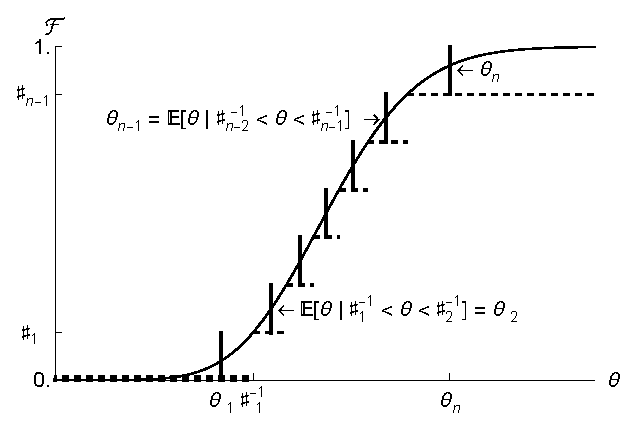
\includegraphics{./Figures/discreteApprox}
    \caption{Equiprobable Discrete Approximation to Lognormal Distribution $\FDist$}
    \label{fig:discreteapprox}
  \end{figure}
\end{verbatimwrite}
\hypertarget{discreteApprox}{}
  \begin{figure}
        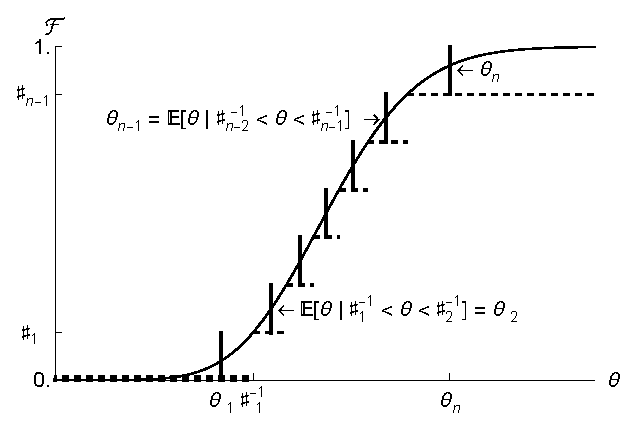
\includegraphics{./Figures/discreteApprox}
        \caption{Discrete Approximation to Lognormal Distribution $\FDist$}
        \label{fig:discreteapprox}
\end{figure}
\unskip
% \write18{cat \econtexRoot/Figures/discreteApprox.tex >> \econtexRoot/Figures/SolvingMicroDSOPs-Figures-List.tex}

Substituting into our definition of $\vEndStget({a}_{t})$, for $t=T-1$
\begin{verbatimwrite}{./Equations/vDiscrete.tex}
  \begin{equation}\begin{gathered}\begin{aligned}
        \vFunc_{T^{+}-1}({a}_{T-1})  & =   \DiscFac \PermGroFac_{t+1}^{1-\CRRA}\left(\frac{1}{n_{\TranShkEmp}}\right)\sum_{i=1}^{n_{\TranShkEmp}}   \frac{\left(\RNrm_{t+1} {a}_{t} + \TranShkEmp_{i}\right)^{1-\CRRA}}{1-\CRRA} \label{eq:vDiscrete}
      \end{aligned}\end{gathered}\end{equation}
\end{verbatimwrite}
\begin{eqnarray}
        \vEnd_{T-1}({a}_{T-1}) & = &   \Discount \PGro_{T}^{1-\CRRA}\left(\frac{1}{n_{\tShkEmp}}\right)\sum_{i=1}^{n_{\tShkEmp}}   \frac{\left( \Rnorm_{T} {a}_{T-1} + \tShkEmp_{i}\right)^{1-\CRRA}}{1-\CRRA} \label{eq:vDiscrete}
\end{eqnarray}
\unskip
so we can rewrite the maximization problem as \ifthenelse{\boolean{MyNotes}}{\marginpar{\tiny Be sure to discuss \eqref{eq:vEndTm1} explicitly, as it is implemented directly in the program as per equation \eqref{eq:vEndTm1prog}.}}{}
\begin{verbatimwrite}{./Equations/vEndTm1.tex}
  \begin{equation}\begin{gathered}\begin{aligned}
        {\vFunc}_{T-1}({m}_{T-1})   & = \max_{\cNrm_{T-1}}
        \left\{
          \frac{{c}_{T-1}^{1-\CRRA}}{1-\CRRA} +
          \vFunc_{T^{+}-1}({m}_{T-1}-{c}_{T-1})
        \right\}.
        \label{eq:vEndTm1}
      \end{aligned}\end{gathered}\end{equation}
\end{verbatimwrite}
\begin{eqnarray}
{\vFunc}_{T-1}({m}_{T-1})  & = & \max_{\cRat_{T-1}}
\left\{
\frac{{c}_{T-1}^{1-\CRRA}}{1-\CRRA} +
\vEnd_{T-1}({m}_{T-1}-{c}_{T-1})
\right\}.
 \label{eq:vEndTm1}
\end{eqnarray}
\unskip

\hypertarget{The-Approximate-Consumption-and-Value-Functions}{}
\subsection{The Approximate Consumption and Value Functions}

Given a particular value of ${m}_{T-1}$, a numerical maximization
routine can now find the ${c}_{T-1}$ that maximizes
\eqref{eq:vEndTm1} in a reasonable amount of time.%  The {\Mma} program that solves exactly this problem is called \texttt{2period.m}.  (The archive also contains parallel Matlab programs, but these notes will dwell on the specifics of the {\Mma} implementation, which is superior in many respects.)

The first thing \texttt{2period.m} does is to read in the file
\texttt{functions.m} which contains definitions of the consumption and
value functions; \texttt{functions.m} also defines the function \texttt{SolveAnotherPeriod}
which, given the existence in memory of a solution for period $t+1$,
solves for period $t$.

The next step is to
run the programs \texttt{setup\_params.m}, \texttt{setup\_grids.m},
\texttt{setup\_shocks.m}, respectively. \texttt{setup\_params.m} sets values for the
parameter values like the coefficient of relative risk aversion.
\texttt{setup\_shocks.m} calculates the values for the $\TranShkEmp_{i}$
defined above (and puts those values, and the (identical) probability associated
with each of them, in the vector variables \texttt{$\TranShkEmp$Vals} and
\texttt{$\TranShkEmp$Prob}).  Finally, \texttt{setup\_grids.m} constructs a
list of potential values of cash-on-hand and saving, then puts them in the vector
variables \texttt{mVec} = \texttt{aVec} = $\{0,1,2,3,4\}$ respectively.
Then \texttt{2period.m} runs the program \texttt{setup\_lastperiod.m}
which defines the elements necessary to determine behavior in the last
period, in which $\cFunc_{T}(m)=m$ and $\vFunc_{T}(m)=\uFunc(m)$.

After all the setup, the only remaining step in
\texttt{2period.m} is to invoke \texttt{SolveAnotherPeriod}, which
constructs the solution for period $T-1$ given the presence of the
solution for period $T$ (constructed by \texttt{setup\_lastperiod.m}).

Because we will always be comparing our solution to the perfect
foresight solution, we also construct the variables required to
characterize the perfect foresight consumption function in periods
prior to $T$.  In particular, we construct the list \texttt{yExpPDV}
(which contains the PDV of expected income -- `expected human
wealth'), and \texttt{yMinPDV} which contains the minimum possible
discounted value of future income at the beginning of period $T-1$
(`minimum human wealth').\footnote{This is useful in determining the
  search range for the optimal level of consumption in the
  maximization problem.}

The perfect foresight consumption function is also constructed
(\texttt{setup\_PerfectForesightSolution.m}).  This program uses the
fact that, in {\Mma}, functions can be saved as objects using the
commands \texttt{\#} and \texttt{\&}. The \texttt{\#} denotes the
argument of the function, while the \texttt{\&}, placed at the end of
the function, tells {\Mma} that the function should be saved as an
object. In the program, the last period perfect foresight consumption
function is saved as an element in the list \texttt{$\cNrm\digamma$ =
  \{(\# - 1 + Last[yExpPDV]) Last[$\kappa$Min] \&\}}, where
\texttt{Last[yExpPDV]} gives the just-constructed PDV of human wealth
at the beginning of $T$ (equal to 1, since current income is included
in $h_{T}$), and \texttt{Last[$\kappa$Min]} gives the perfect
foresight marginal propensity to consume (equal to 1, since it is
optimal to spend all resources in the last period). Since \texttt{\#}
in the code stands in for what was called $m$ in the model, the
discounted total wealth is decomposed into discounted non-human wealth
\texttt{\# - 1} and discounted human wealth
\texttt{Last[yExpPDV]}. The resulting formula then corresponds to
$\bar{\cFunc}_{T} = (m_{T}-1+{h}_{T})\MPCmin_{T}$, which translates to
$\bar{\cFunc}_{T} = m_{T}$ for ${h}_{T}=\MPCmin_{T}=1$.

The infinite horizon perfect foresight marginal propensity to save 
\begin{equation}\begin{gathered}\begin{aligned}
      \MPS  & = (1/\Rfree)(\Rfree \DiscFac)^{1/\CRRA} \label{eq:lambdadefn}
    \end{aligned}\end{gathered}\end{equation}
is also defined because it will be useful in a number of derivations.\footnote{Detailed discussion can
  be found in Carroll~\citeyearpar{BufferStockTheory}.}

The program then constructs behavior for one iteration back from the
last period of life by using the function
\texttt{AddNewPeriodToParamLifeDates}.  Using the {\Mma}~command
\texttt{AppendTo}, various existing lists (which characterized the
solution for period $T$) are redefined to include an additional
element representing the relevant formulas in the second to last
period of life. For example, \texttt{$\kappa$Min} now has two
elements.  The second element, given by \texttt{1/(1 +
  Last[$\MPS$]/Last[$\kappa$Min])}, is the perfect foresight marginal
propensity to consume in $t=T-1$.\footnote{Carroll~\citeyearpar{BufferStockTheory} shows that this is also a
  recurring formula that extends inductively to earlier periods.}

Next, the program defines a function \texttt{$\vEndStget$[at\_]} (in \texttt{functions\_stable.m})
which \ifthenelse{\boolean{MyNotes}}{\marginpar{\tiny General rule:
    functions with `Raw' in the name are exact representations of some
    theoretical construct in the text.}}{} is the exact implementation
of (\ref{eq:vEndtdefn}): It returns the expectation of
the value of behaving optimally in period $T$ given any specific
amount of assets at the end of $T-1$, ${a}_{T-1}$.

The heart of the program is the next expression
(in \texttt{functions.m}).
This expression
loops over the values of the variable \texttt{mVec}, solving the
maximization problem
(given in  equation (\ref{eq:vEndTm1})):\ifthenelse{\boolean{MyNotes}}{\marginpar{\tiny This corresponds exactly to equation \eqref{eq:vEndTm1}.}}{}
\begin{equation}\begin{gathered}\begin{aligned}
      \max_{\texttt{c}} &  & \mbox{\texttt{u[c] + $\vEndStget$[mVec[[i]]-c]}} \label{eq:vEndTm1prog}
    \end{aligned}\end{gathered}\end{equation}
for each of the $i$ values of \texttt{mVec} (henceforth let's
call these points ${m}_{T-1,i}$).
\ifthenelse{\boolean{MyNotes}}{\marginpar{\tiny Clarify the
    {\Mma} syntax that only the last item in the expression becomes
    the table entry.  Lines 14-18 solve and put the result in cSoln.}}{}
The maximization routine returns two values: the maximized value,
and the value of ${c}$ which yields that maximized value.
When the loop (the \texttt{Table} command) is finished, the variable
\texttt{vAndcList} contains two lists, one with the values
$\vNrm_{T-1,i}$ and the other with the consumption levels
${c}_{T-1,i}$ associated with the ${m}_{T-1,i}$.
\ifthenelse{\boolean{MyNotes}}{\marginpar{\tiny The expression
    $\{$cSoln[[1]],(c /. cSoln[[2]])$\}$ extracts the results. The
    Transpose commands extract the first and second columns.}}{}

\hypertarget{an-interpolated-consumption-function}{}
\subsection{An Interpolated Consumption Function} \label{subsec:LinInterp}

Given a set of points on a function (in this case, the consumption function $\cFunc_{T-1}(\mNrm)$), we can create an object called an `interpolating function' which when applied to an input ${m}$ will yield the value of $\cNrm$ that corresponds to a linear `connect-the-dots' interpolation of the value of $\cNrm$ from the points, creating a function that aims to provide an approximation of the functions whose points have been sampled.  We will do this to define an approximation to the consumption function $\Alt{\cFunc}_{T-1}({m}_{T-1})$ which, when called with an ${m}_{T-1}$ that is equal to one of the points in \texttt{mVec[[i]]} returns the associated value of ${c}_{T-1,i}$, and when called with a value of ${m}_{T-1}$ that is not exactly equal to one of the \texttt{mVec[[i]]}, returns the value of ${c}$ that reflects a linear interpolation between the ${c}_{T-1,i}$ associated with the two \texttt{mVec[[i]]} points nearest to ${m}_{T-1}$.  Thus if the function is called with ${m}_{T-1} = 1.75$ and the nearest gridpoints \ifthenelse{\boolean{MyNotes}}{\marginpar{\tiny Go to the optimal consumption figure and show the connect-the-dots; point out that it's more obvious for the ${\vFunc}_{T-1}$.}}{} are ${m}_{j,T-1}=1$ and ${m}_{k,T-1}=2$ then the value of ${c}_{T-1}$ returned by the function would be $(0.25 {c}_{j,T-1}+0.75 {c}_{k,T-1})$. We can define a numerical approximation to the value function $\Alt{\vFunc}_{T-1}({m}_{T-1})$ in an exactly analogous way.


Figures \ref{fig:PlotcTm1Simple} and~\ref{fig:PlotVTm1Simple} show
plots of the $\Alt{\cFunc}_{T-1}$ and $\Alt{\vFunc}_{T-1}$
\texttt{InterpolatingFunctions} that are generated by the program
\texttt{2PeriodInt.m}.  While the $\Alt{\cFunc}_{T-1}$ function looks
very smooth, the fact that the $\Alt{\vFunc}_{T-1}$ function is a set
of line segments is very evident.  This figure provides the beginning
of the intuition for why trying to approximate the value function
directly is a bad idea (in this context).\footnote{For some problems,
  especially ones with discrete choices, value function approximation is unavoidable;
  nevertheless, even in such problems, the techniques sketched below can
  be very useful across much of the range over which the problem is defined.}

\hypertarget{PlotcTm1Simple}{}
\begin{figure}
  \centerline{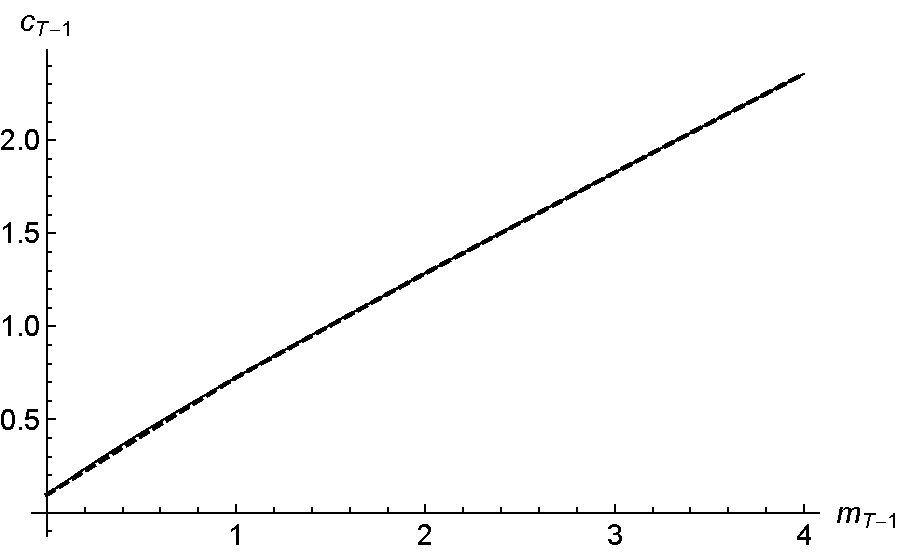
\includegraphics{./Figures/PlotcTm1Simple}}
  \caption{$\cFunc_{T-1}({m}_{T-1})$ (solid) versus $\Alt{\cFunc}_{T-1}({m}_{T-1})$ (dashed)}
  \label{fig:PlotcTm1Simple}
\end{figure}

\hypertarget{PlotvTm1Simple}{}
\begin{figure}
  \centerline{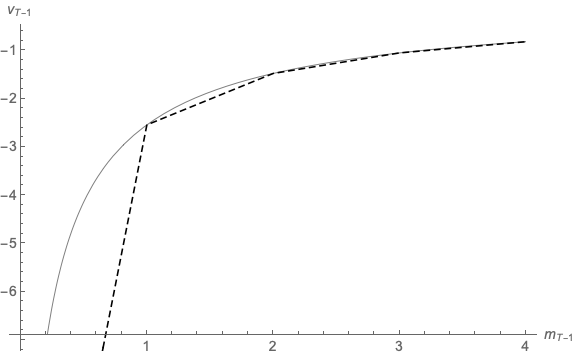
\includegraphics{./Figures/PlotVTm1Simple}}
  \caption{$\vFunc_{T-1}$ (solid) versus $\Alt{\vFunc}_{T-1}({m}_{T-1})$ (dashed)}
  \label{fig:PlotVTm1Simple}
\end{figure}

\hypertarget{Interpolating-Expectations}{}
\subsection{Interpolating Expectations}

\ifthenelse{\boolean{MyNotes}}{\marginpar{\tiny Good approximation in the sense that increasing the number of points makes no discernable difference.}}{}

\texttt{2period.m} works well in the sense that it
generates a good approximation to the true optimal consumption
function.  However, there is a clear inefficiency in the program:
Since it uses equation \eqref{eq:vEndTm1}, for every value
of ${m}_{T-1}$ the program must calculate the utility consequences of
various possible choices of $\cNrm_{T-1}$ as it searches for the best choice.
\ifthenelse{\boolean{MyNotes}}{\marginpar{\tiny Problem:
    \eqref{eq:maxprob2} means for every ${m}_{T-1}$ calc the value of
    $\cFunc_{T-1}$; for a given ${a}_{T-1}$ (say 0) the value may be
    calculated many times.}}{} But for any given value of ${a}_{T-1}$,
there is a good chance that the program may end up calculating the
corresponding $\vEndStget$ many times while maximizing utility from different
${m}_{T-1}$'s.  For example, it is possible that the program will
calculate the value of ending the period with ${a}_{T-1}=0$ dozens of times.  It would
be much more efficient if the program could make that calculation once
and then merely recall the value when it is needed again.

This can be achieved using the same interpolation technique used above
to construct a direct numerical approximation to the value function:
Define a grid of possible values for saving at time $T-1$,
$\vec{a}_{T-1}$
(\texttt{aVec}
in \texttt{setup\_grids.m}), designating the
specific points $\null{a}_{T-1,i}$; for each of these values of
$\null{a}_{T-1,i}$, calculate the vector $\vec{\vFunc}_{T^{+}-1}$ as the collection of points $\vFunc_{T^{+}-1,i} =
\vFunc_{T^{+}-1}(\null{a}_{T-1,i})$ using equation
(\ref{eq:vEndtdefn}); then construct an
\texttt{InterpolatingFunction} object
$\Alt{\vFunc}_{T^{+}-1}({a}_{T-1})$ from the list of 
points on the function captured in the $\vec{a}_{T-1}$ and $\vec{\vFunc}_{T^{+}-1}$ vectors.

Thus, we are now interpolating for the function 
that reveals the expected value of \textit{ending} the period with a given amount
of assets.\footnote{What we are doing here is closely related to `the
  method of parameterized expectations' of
  \cite{denHaanMarcet:parameterized}; the only difference is that our
  method is essentially a nonparametric version.}  The
program \texttt{2periodIntExp.m} solves this problem.  Figure~\ref{fig:PlotOTm1RawVSInt} compares the true value function to the
\texttt{InterpolatingFunction} approximation; the functions are of course
identical at the gridpoints chosen for ${a}_{T-1}$ and they appear
reasonably close except in the region below
${m}_{T-1}=1$.

\hypertarget{PlotOTm1RawVSInt}{}
\begin{figure}
  \centerline{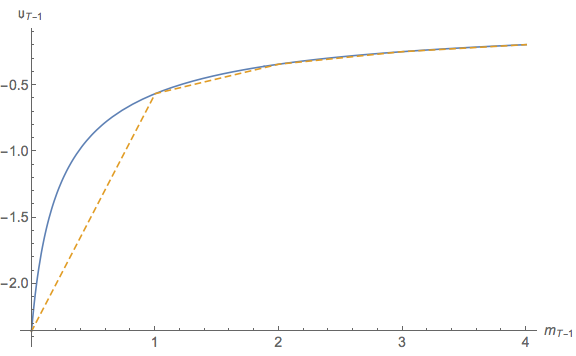
\includegraphics{./Figures/PlotOTm1RawVSInt}}
  \caption{End-Of-Period Value $\vFunc_{T^{+}-1}({a}_{T-1})$ (solid) versus $\Alt{\vFunc}_{T^{+}-1}({a}_{T-1})$ (dashed)}
  \label{fig:PlotOTm1RawVSInt}
\end{figure}

\hypertarget{PlotComparecTm1AB}{}
\begin{figure}
  \centerline{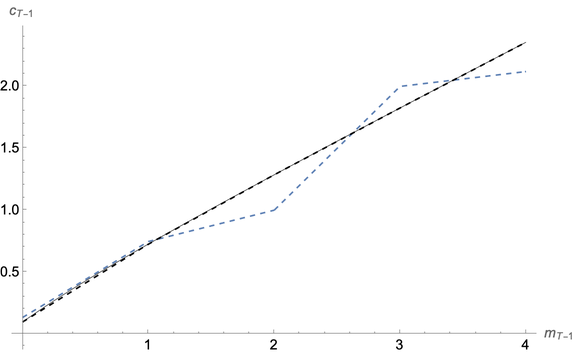
\includegraphics{./Figures/PlotComparecTm1AB}}
  \caption{$\cFunc_{T-1}({m}_{T-1})$ (solid) versus $\Alt{\cFunc}_{T-1}({m}_{T-1})$ (dashed)}
  \label{fig:PlotComparecTm1AB}
\end{figure}

Nevertheless, the resulting consumption rule obtained when $\Alt{\vFunc}_{T^{+}-1}({a}_{T-1})$
is used\ifthenelse{\boolean{MyNotes}}{\marginpar{\tiny Don't skip the 2-3-3-4
    example in the text - it will be used again in a moment.}}{}
instead of $\vFunc_{T^{+}-1}({a}_{T-1})$ is surprisingly bad, as
shown in figure \ref{fig:PlotComparecTm1AB}.  For example, when
${m}_{T-1}$ goes from 2 to 3, $\Alt{\cFunc}_{T-1}$ goes from about 1
to about 2, yet when ${m}_{T-1}$ goes from 3 to 4, $\Alt{\cNrm}_{T-1}$
goes from about 2 to about 2.05.  The function fails even to be
strictly concave, which is distressing because Carroll and
Kimball~\citeyearpar{ckConcavity} prove that the correct
consumption function is strictly concave in a wide class of problems that
includes this problem.

\hypertarget{Value-Function-versus-First-Order-Condition}{}
\subsection{Value Function versus First Order Condition}\label{subsec:vVsuP}

Loosely speaking, our difficulty reflects the fact that the
consumption choice is governed by the \textit{marginal} value function,
not by the \textit{level} of the value function (which is the object that
we approximated).  To understand this point, recall that a quadratic
utility function\ifthenelse{\boolean{MyNotes}}{\marginpar{\tiny
    Intuitively speaking, if one's goal is to accurately capture
    behavior that is governed by marginal utility or the marginal
    value function, numerical techniques that approximate the \textit{
      marginal} value function are likely to work better.}}{} exhibits
risk aversion because with a stochastic ${c}$,
\begin{equation}
  \Ex[-({c} - \cancel{c})^{2}] < - (\Ex[{c}] - \cancel{c})^{2}
\end{equation}
where $\cancel{c}$ is the `bliss point'. However, unlike the CRRA utility function,
with quadratic utility the consumption/saving \textit{behavior} of consumers
is unaffected by risk since behavior is determined by the first order condition, which
depends on \textit{marginal} utility, and when utility is quadratic, marginal utility is unaffected
by risk:
\begin{equation}
  \Ex[-2({c} - \cancel{c})] = - 2(\Ex[{c}] - \cancel{c}).
\end{equation}

Intuitively, if one's goal is to accurately capture choices
that are governed by marginal value,
numerical techniques that approximate the \textit{marginal} value
function will yield a more accurate approximation to
optimal behavior than techniques that approximate the \textit{level}
of the value function.

The first order condition of the maximization problem in period $T-1$ is:
\begin{verbatimwrite}{./Equations/FOCTm1.tex}
  \begin{equation}\begin{gathered}\begin{aligned}
        \uFunc^{{c}}({c}_{T-1})       & = \DiscFac \Ex_{T-1} [\PermGroFac_{T}^{-\CRRA}\Rfree \uFunc^{{c}}({c}_{T})]  %\label{eq:focraw}
        \\      {c}_{T-1}^{-\CRRA}   & = \Rfree \DiscFac \left(\frac{1}{n_{\TranShkEmp}}\right) \sum_{i=1}^{n_{\TranShkEmp}} \PermGroFac_{T}^{-\CRRA}\left(\Rfree ({m}_{T-1}-{c}_{T-1}) + \TranShkEmp_{i}\right)^{-\CRRA} \label{eq:FOCTm1}.
      \end{aligned}\end{gathered}\end{equation}
\end{verbatimwrite}
\begin{eqnarray}
    \util^{\prime}({c}_{T-1})      & = & \Discount \Ex_{T-1} [\PGro_{T}^{-\CRRA}\Rfree \util^{\prime}({c}_{T})]  \label{eq:focraw}
\\      {c}_{T-1}^{-\CRRA}  & = & \Rfree \Discount \left(\frac{1}{n_{\tShkEmp}}\right) \sum_{i=1}^{n_{\tShkEmp}} \PGro_{T}^{-\CRRA}\left(\Rfree ({m}_{T-1}-{c}_{T-1}) + \tShkEmp_{i}\right)^{-\CRRA} \label{eq:FOCTm1}.
\end{eqnarray}
\unskip
\ifthenelse{\boolean{MyNotes}}{\marginpar{\tiny Go from the first to the last equation in \eqref{eq:FOCTm1} by substituting $\uFunc(c)=c^{-\CRRA}$ and use the approximation to the integral.}}{}
\hypertarget{PlotuPrimeVSOPrime}{}
\begin{figure}
  \centerline{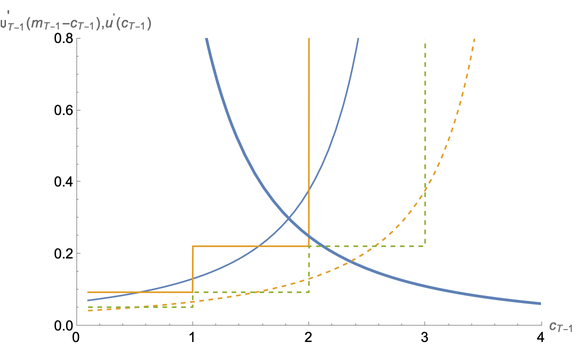
\includegraphics{./Figures/PlotuPrimeVSOPrime}}
  \caption{$\uFunc^{{c}}(c)$ versus $\vFunc_{T^{+}-1}^{{a}}(3-c), \vFunc_{T^{+}-1}^{{a}}(4-c), \Alt{\vFunc}_{T^{+}-1}^{{a}}(3-c), \Alt{\vFunc}_{T^{+}-1}^{{a}}(4-c)$}
  \label{fig:PlotuPrimeVSOPrime}
\end{figure}

The downward-sloping curve in Figure \ref{fig:PlotuPrimeVSOPrime}
shows the value of ${c}_{T-1}^{-\CRRA}$ for our baseline parameter values
for $0 \leq {c}_{T-1} \leq 4$ (the horizontal axis).  The solid
upward-sloping curve shows the value of the RHS of (\ref{eq:FOCTm1})
as a function of ${c}_{T-1}$ under the assumption that ${m}_{T-1}=3$.
Constructing this figure is rather time-consuming, because for every
value of ${c}_{T-1}$ plotted we must calculate the RHS of
(\ref{eq:FOCTm1}).  The value of ${c}_{T-1}$ for which the RHS and LHS
of (\ref{eq:FOCTm1}) are equal is the optimal level of consumption
given that ${m}_{T-1}=3$, so the intersection of the downward-sloping
and the upward-sloping curves gives the optimal value of ${c}_{T-1}$.
As we can see, the two curves intersect just below ${c}_{T-1}=2$.
Similarly, the upward-sloping dashed curve shows the expected value
of the RHS of (\ref{eq:FOCTm1}) under the assumption that ${m}_{T-1}=4$,
and the intersection of this curve with $\uFunc^{{c}}({c}_{T-1})$ yields the
optimal level of consumption if ${m}_{T-1}=4$.  These two curves
intersect slightly below ${c}_{T-1}=2.5$.  Thus, increasing ${m}_{T-1}$
from 3 to 4 increases optimal consumption by about 0.5.

\ifthenelse{\boolean{MyNotes}}{\marginpar{\tiny Flip back to Figure
    4 to make the point that $\Alt{\vEndStget}^{{a}}$ is a step
    function.}}{} Now consider the derivative of our function
$\Alt{\vFunc}_{T^{+}-1}({a}_{T-1})$.  Because we have constructed
$\Alt{\vFunc}_{T^{+}-1}$ as a linear interpolation, the slope of
$\Alt{\vFunc}_{T^{+}-1}({a}_{T-1})$ between any two adjacent
points $\{\null{a}_{T-1,i},{a}_{i+1,T-1}\}$ is constant.  The
level of the slope immediately below any particular gridpoint is
different, of course, from the slope above that gridpoint, a fact
which implies that the derivative of
$\Alt{\vFunc}_{T^{+}-1}({a}_{T-1})$ follows a step function.

The solid-line step function in Figure \ref{fig:PlotuPrimeVSOPrime}
depicts the actual value of
$\Alt{\vFunc}_{T^{+}-1}^{{a}}(3-{c}_{T-1})$.  When we attempt to find
optimal values of ${c}_{T-1}$ given ${m}_{T-1}$ using
$\Alt{\vFunc}_{T^{+}-1}({a}_{T-1})$, the numerical optimization
routine will return the ${c}_{T-1}$ for which $\uFunc^{{c}}({c}_{T-1}) =
\Alt{\vFunc}^{{a}}_{T^{+}-1}({m}_{T-1}-{c}_{T-1})$.  Thus, for
${m}_{T-1}=3$ the program will return the value of ${c}_{T-1}$ for
which the downward-sloping $\uFunc^{{c}}({c}_{T-1})$ curve intersects with the
$\Alt{\vFunc}_{T^{+}-1}^{{a}}(3-{c}_{T-1})$; as the diagram shows,
this value is exactly equal to 2.  Similarly, if we ask the routine
to find the optimal ${c}_{T-1}$ for ${m}_{T-1}=4$, it finds the point
of intersection of $\uFunc^{{c}}({c}_{T-1})$ with
$\Alt{\vFunc}_{T^{+}-1}^{{a}}(4-{c}_{T-1})$; and as the diagram shows,
this intersection is only slightly above 2.  Hence, this figure
illustrates why the numerical consumption function plotted earlier
returned values very close to ${c}_{T-1}=2$ for both ${m}_{T-1}=3$ and
${m}_{T-1}=4$.

We would obviously obtain much better estimates of the point of
intersection between $\uFunc^{{c}}({c}_{T-1})$ and
$\vFunc_{T^{+}-1}^{{a}}({m}_{T-1}-{c}_{T-1})$ if our estimate of
$\Alt{\vFunc}^{{a}}_{T^{+}-1}$ were not a step function.  In
fact, we already know how to construct linear interpolations
to functions, so the obvious next step is to construct a
linear interpolating approximation to the \textit{expected marginal
  value of end-of-period assets function} $\vEndStget^{\prime}$. That is, we calculate
\begin{equation}\begin{gathered}\begin{aligned}
      \vFunc_{T^{+}-1}^{{a}}({a}_{T-1})  & =  \DiscFac \Rfree \PermGroFac_{T}^{-\CRRA} \left(\frac{1}{n_{\TranShkEmp}}\right) \sum_{i=1}^{n_{\TranShkEmp}} \left(\RNrm_{T} {a}_{T-1} + \TranShkEmp_{i}\right)^{-\CRRA} \label{eq:vEndPrimeTm1}
    \end{aligned}\end{gathered}\end{equation}
at the points in \texttt{aVec} yielding
$\{\{\null{a}_{T-1,1},\vFunc_{T^{+}-1,1}^{{a}}\},\{{a}_{T-1,2},\vFunc_{T^{+}-1,2}^{{a}}\}
\ldots\}$ and construct
$\Alt{\vFunc}_{T^{+}-1}^{{a}}({a}_{T-1})$ as the linear
interpolating function that fits this set of points.

\hypertarget{PlotOPRawVSFOC}{}
\begin{figure}
  \centerline{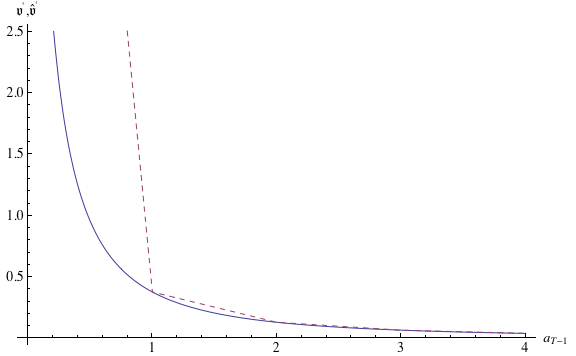
\includegraphics{./Figures/PlotOPRawVSFOC}}
  \caption{$\vFunc_{T^{+}-1}^{{a}}({a}_{T-1})$ versus $\Alt{\vFunc}_{T^{+}-1}^{{a}}({a}_{T-1})$}
  \label{fig:PlotOPRawVSFOC}
\end{figure}


The program file \texttt{functionsIntExpFOC.m} therefore
uses the function \texttt{vEndStgeta[at\_]} defined in \texttt{functions\_stable.m}
as the embodiment of equation~(\ref{eq:vEndPrimeTm1}), and constructs the
\texttt{InterpolatingFunction} as described above.  The results are
shown in Figure \ref{fig:PlotOPRawVSFOC}.  The linear
interpolating approximation looks roughly as good (or bad) for the
\textit{marginal} value function as it was for the level of the value
function. However, Figure \ref{fig:PlotcTm1ABC} shows that the new
consumption function (long dashes) is a considerably better
approximation of the true consumption function (solid) than was the
consumption function obtained by approximating the level of the
value function (short dashes).

\hypertarget{PlotcTm1ABC}{}
\begin{figure}
  \centerline{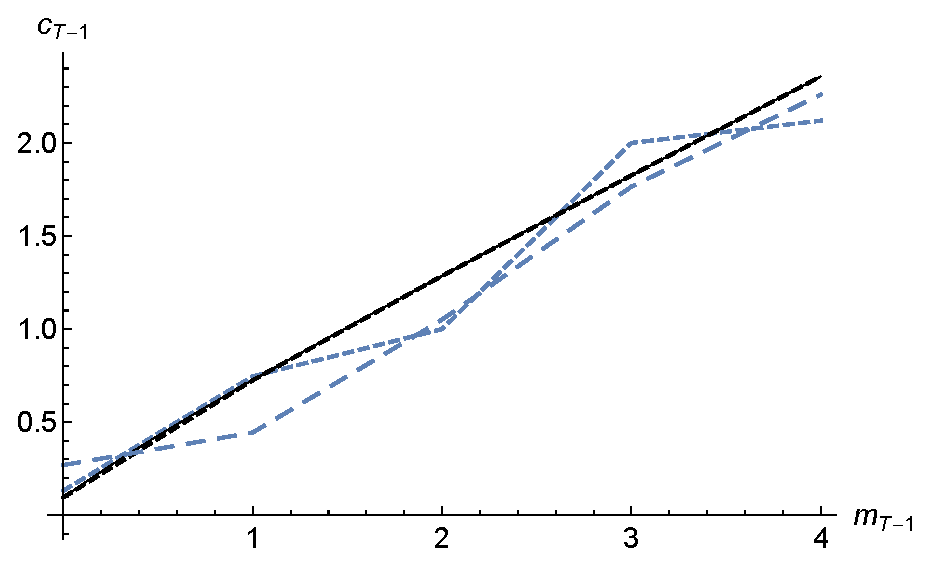
\includegraphics{./Figures/PlotcTm1ABC}}
  \caption{$\cFunc_{T-1}({m}_{T-1})$ (solid) Versus Two Methods for Constructing $\Alt{\cFunc}_{T-1}({m}_{T-1})$}
  \label{fig:PlotcTm1ABC}
\end{figure}

\hypertarget{Transformation}{}
\subsection{Transformation}

Even the new-and-improved consumption function diverges notably from the true
solution, especially at lower values of ${m}$.  That is because the
linear interpolation does an increasingly poor job of capturing the
nonlinearity of $\vFunc_{T^{+}-1}^{{a}}({a}_{T-1})$ at
lower and lower levels of ${a}$.

This is where we unveil our next trick.  To understand the logic,
start by considering the case where $\RNrm_{T} = \DiscFac =
\PermGroFac_{T} = 1$ and there is no uncertainty
\ifthenelse{\boolean{MyNotes}}{\marginpar{\tiny Go over this
    carefully.}}{} (that is, we know for sure that income next period
will be $\TranShkEmp_{T} = 1$).  The final Euler equation is then:
\begin{equation}\begin{gathered}\begin{aligned}
      {c}_{T-1}^{-\CRRA}  & = {c}_{T}^{-\CRRA}.
    \end{aligned}\end{gathered}\end{equation}

In the case we are now considering with no uncertainty and no liquidity
constraints, the optimizing consumer does not care whether a unit of
income is scheduled to be received in the future period $T$ or the
current period $T-1$; there is perfect certainty that the income will
be received, so the consumer treats it as equivalent to a unit of
current wealth.  Total resources therefore are comprised of two types:
current market resources ${m}_{T-1}$ and `human wealth' (the PDV of
future income) of $\hEnd_{T-1}=1$ (where we use the Gothic font to
signify that this is the expectation, as of the END of the period, of
the income that will be received in future periods; it does not
include current income, which has already been incorporated into
${m}_{T-1}$).

The optimal solution is to spend half of total lifetime resources in
period $T-1$ and the remainder in period $T$.  Since total resources
are known with certainty to be
${m}_{T-1}+\hEnd_{T-1}= {m}_{T-1}+1$, and since
${\vFunc}_{T-1}^{{m}}({m}_{T-1}) = \uFunc^{{c}}({c}_{T-1})$ this
implies that \ifthenelse{\boolean{MyNotes}}{\marginpar{\tiny Crucial
    point: this is \textit{marginal} value function in period $T-1$,
    which we were trying to approximate with a linear interpolating
    function earlier.}}{}
\begin{equation}
  \vFunc^{{m}}_{T-1}({m}_{T-1})  = \left(\frac{{m}_{T-1}+1}{2}\right)^{-\CRRA} \label{eq:vPLin}.
\end{equation}
Of course, this is a highly nonlinear
function.  However, if we raise both sides of \eqref{eq:vPLin} to the
power $(-1/\CRRA)$ the result is a linear function:
\begin{equation}\begin{gathered}\begin{aligned}
      [\vFunc^{{m}}_{T-1}({m}_{T-1})]^{-1/\CRRA}  & = \frac{{m}_{T-1}+1}{2}  .
    \end{aligned}\end{gathered}\end{equation}
This is a specific example of a general phenomenon: A theoretical
literature cited in~\cite{ckConcavity} establishes that under
perfect certainty, if the period-by-period marginal utility function
is of the form ${c}_{t}^{-\CRRA}$, the marginal value function will be
of the form $(\gamma {m}_{t}+\zeta)^{-\CRRA}$ for some constants
$\{\gamma,\zeta\}$.  This means that if we were solving the perfect
foresight problem numerically, we could always calculate a numerically
exact (because linear) interpolation.  To put this in intuitive terms,
the problem we are facing is that the marginal value function is
highly nonlinear.  But we have a compelling solution to that problem,
because the nonlinearity springs largely from the fact that we are raising
something to the power $-\CRRA$.  In effect, we can `unwind' all of
the nonlinearity owing to that operation and the remaining
nonlinearity will not be nearly so great.  Specifically, applying the foregoing insights
to the end-of-period value function $\vFunc^{{a}}_{T^{+}-1}({a}_{T-1})$, we can define
\begin{equation}\begin{gathered}\begin{aligned}
      \cFunc_{T^{+}-1}({a}_{T-1})  & \equiv  \left(\vFunc^{{a}}_{T^{+}-1}({a}_{T-1})\right)^{-1/\CRRA} \label{eq:cGoth}
    \end{aligned}\end{gathered}\end{equation}
which would be linear in the perfect foresight case.  Thus, our
procedure is to calculate the values of $\cFunc_{T^{+}-1,i}$ at each
of the ${a}_{T-1,i}$ gridpoints, with the idea that we will construct
$\Alt{\cFunc}_{T^{+}-1}$ as the interpolating function connecting
these
points.  % A comparison of the result to the true consumed function is presented in figure~\ref{fig:GothVInvVSGothC}.  The two solutions are quite close.


\hypertarget{The-Natural-Borrowing-Constraint-and-the-a-Lower-Bound}{}
\subsection{The `Natural' Borrowing Constraint and the $a_{T-1}$ Lower Bound} \label{subsec:LiqConstrSelfImposed}


This is the appropriate moment to ask an awkward question we have so far
neglected: How should a function like $\Alt{\cFunc}_{T^{+}-1}$
be evaluated outside the range of points spanned by
$\{{a}_{T-1,1},...,{a}_{T-1,n}\}$ for which we have calculated
the corresponding $\cFunc_{T^{+}-1,i}$ gridpoints used to produce our
linearly interpolating approximation $\Alt{\cFunc}_{T^{+}-1}$ (as described in section~\ref{subsec:LinInterp})?

The natural answer would seem to be linear extrapolation; for example, we could use
\begin{equation}\begin{gathered}\begin{aligned}
      \Alt{\cFunc}_{T^{+}-1}({a}_{T-1})  & = \Alt{\cFunc}_{T^{+}-1}({a}_{T-1,1})+\Alt{\cFunc}_{T^{+}-1}^{{a}}({a}_{T-1,1})({a}_{T-1}-{a}_{T-1,1}) \label{eq:ExtrapLin}
    \end{aligned}\end{gathered}\end{equation}
for values of ${a}_{T-1} < {a}_{T-1,1}$, where $\Alt{\cFunc}_{T^{+}-1}^{{a}}({a}_{T-1,1})$ is the derivative of the $\Alt{\cFunc}_{T^{+}-1}$ function at the bottommost gridpoint (see below).  Unfortunately, this approach
will lead us into difficulties.  To see why, consider what
happens to the true (not approximated) $\vFunc^{{a}}_{T^{+}-1}({a}_{T-1})$ as
${a}_{T-1}$ approaches the value
$\underline{a}_{T-1}=-\underline{\TranShkEmp}\RNrm_{T}^{-1}$.  From
\eqref{eq:vEndPrimeTm1} we have
\begin{equation}\begin{gathered}\begin{aligned}
      \lim_{{a}_{T-1} \downarrow \underline{a}_{T-1}} \vFunc^{{a}}_{T^{+}-1}({a}_{T-1}) 
      & =                                                                                         \lim_{{a}_{T-1} \downarrow \underline{a}_{T-1}} \DiscFac \Rfree \PermGroFac_{T}^{-\CRRA} \left(\frac{1}{n_{\TranShkEmp}}\right) \sum_{i=1}^{n_{\TranShkEmp}} \left( {a}_{T-1} \RNrm_{T}+ \TranShkEmp_{i}\right)^{-\CRRA}.
    \end{aligned}\end{gathered}\end{equation}

\providecommand{\TranShkEmpMin}{}\renewcommand{\TranShkEmpMin}{\underline{\TranShkEmp}}
But since $\TranShkEmpMin=\TranShkEmp_{1}$, exactly at
${a}_{T-1}=\underline{a}_{T-1}$ the first term in the summation would
be $(-\TranShkEmpMin+\TranShkEmp_{1})^{-\CRRA}=1/0^{\CRRA}$ which is
infinity.  The reason is simple: $-\underline{a}_{T-1}$ is
the PDV, as of $T-1$, of the minimum possible realization of income in
period $T$ ($\RNrm_{T}\underline{a}_{T-1} = -\TranShkEmp_{1}$).  Thus,
if the consumer borrows an amount greater than or equal to
$\underline{\TranShkEmp}\RNrm_{T}^{-1}$ (that is, if the consumer ends
$T-1$ with ${a}_{T-1} \leq -\underline{\TranShkEmp}\RNrm_{T}^{-1}$) and
then draws the worst possible income shock in period $T$, they will have
to consume zero in period $T$ (or a negative amount), which yields
$-\infty$ utility and $\infty$ marginal utility (or undefined utility
and marginal utility).

These reflections lead us to the conclusion that the consumer faces a
`self-imposed' liquidity constraint (which results from the
precautionary motive): They will never borrow an amount greater
than or equal to $\underline{\TranShkEmp}\RNrm_{T}^{-1}$ (that is,
assets will never reach the lower bound of
$\underline{a}_{T-1}$).\footnote{Another term for a constraint of this
  kind is the `natural borrowing constraint.'}  The constraint is
`self-imposed' in the sense that if the utility function were
different (say, Constant Absolute Risk Aversion), the consumer would
be willing to borrow more than $\underline{\TranShkEmp}\RNrm_{T}^{-1}$
because a choice of zero or negative consumption in period $T$ would
yield some finite amount of utility.\footnote{Though it is very unclear what a
  proper economic interpretation of negative consumption might be --
  this is an important reason why CARA utility, like quadratic utility,
  is increasingly not used for serious quantitative work, though it is
  still useful for teaching purposes.}

This self-imposed constraint cannot be captured well when the
$\vFunc^{{a}}_{T^{+}-1}$ function is approximated by a piecewise
linear function like $\Alt{\vFunc}^{{m}}_{T^{+}-1}$, because a
linear approximation can never reach the correct gridpoint for
$\vFunc^{{a}}_{T^{+}-1}(\underline{a}_{T-1})=\infty.$ To see what
will happen instead, note first that if we are approximating $\vFunc^{{a}}_{T^{+}-1}$ the smallest value in
\texttt{aVec} must be greater than $\underline{a}_{T-1}$
(because the expectation for any gridpoint $\leq \underline{a}_{T-1}$ is undefined).  Then when the
approximating $\vFunc^{{a}}_{T^{+}-1}$ function is evaluated at
some value less than the first element in \texttt{aVec[1]}, the
approximating function will linearly extrapolate the slope that
characterized the lowest segment of the piecewise linear approximation
(between \texttt{aVec[1]} and \texttt{aVec[2]}), a
procedure that will return a positive finite number, even if the
requested ${a}_{T-1}$ point is below $\underline{a}_{T-1}$.  This means that the
precautionary saving motive is understated, and by an arbitrarily
large amount as the level of assets approaches its true theoretical
minimum $\underline{a}_{T-1}$.

The foregoing logic demonstrates that the marginal value of saving approaches infinity as ${a}_{T-1} \downarrow
\underline{a}_{T-1}=-\underline{\TranShkEmp}\RNrm_{T}^{-1}$.  But this
implies that $\lim_{{a}_{T-1} \downarrow \underline{a}_{T-1}}
\cFunc_{T^{+}-1}({a}_{T-1}) = (\vFunc^{{a}}_{T^{+}-1}({a}_{T-1}))^{-1/\CRRA} = 0$;
that is, as ${a}$ approaches its minimum possible value, the
corresponding amount of ${c}$ must approach \textit{its} minimum possible value: zero.

The upshot of this discussion is a realization that all we need to do is to
augment each of the $\vec{a}_{T-1}$ and $\vec{c}_{T-1}$ vectors with an extra point so that the
first element in the list used to produce our \texttt{InterpolatingFunction} is
$\{{a}_{T-1,0},{c}_{T-1,0}\}=\{\underline{a}_{T-1},0.\}$.

\hypertarget{GothVInvVSGothC}{}
\begin{figure}
  \centerline{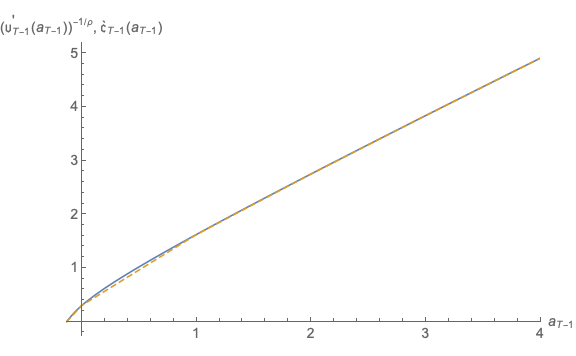
\includegraphics{./Figures/GothVInvVSGothC}}
  \caption{$\cFunc_{T^{+}-1}({a}_{T-1})$ versus $\Alt{\cFunc}_{T^{+}-1}({a}_{T-1})$}
  \label{fig:GothVInvVSGothC}
\end{figure}



Figure\ifthenelse{\boolean{MyNotes}}{\marginpar{\tiny True $\cEndFunc$ is solid, linear approx is dashed.}}{} \ref{fig:GothVInvVSGothC} plots the results (generated by the program \texttt{2periodIntExpFOCInv.m}).  The solid line calculates the exact numerical value of $\cFunc_{T^{+}-1}({a}_{T-1})$ while the dashed line is the linear interpolating approximation $\Alt{\cFunc}_{T^{+}-1}({a}_{T-1}).$ This figure illustrates the value of the transformation: The true function is close to linear, and so the linear approximation is almost indistinguishable from the true function except at the very lowest values of ${a}_{T-1}$.

Figure~\ref{fig:GothVVSGothCInv} similarly shows that when we generate
$\Alt{\Alt{\vFunc}}_{T^{+}-1}^{\prime}({a}_{T-1})$ as
$[\Alt{\cFunc}_{T^{+}-1}({a}_{T-1})]^{-\CRRA}$ (dashed line) we
obtain a \textit{much} closer approximation to the true function
$\vFunc^{{a}}_{T^{+}-1}({a}_{T-1})$ (solid line) than we did in
the previous program which did not do the
transformation (Figure~\ref{fig:PlotOPRawVSFOC}).

\hypertarget{GothVVSGothCInv}{}
\begin{figure}
  \centerline{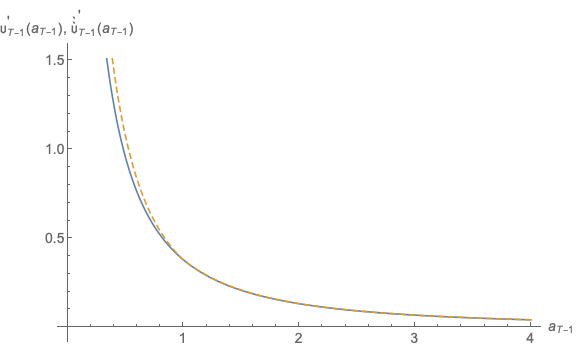
\includegraphics{./Figures/GothVVSGothCInv}}
  \caption{$\vFunc^{{a}}_{T^{+}-1}({a}_{T-1})$ vs. $\Alt{\Alt{\vFunc}}_{T^{+}-1}^{\prime}({a}_{T-1})$ Constructed Using $\Alt{\cFunc}_{T^{+}-1}({a}_{T-1})$}
  \label{fig:GothVVSGothCInv}
\end{figure}



\hypertarget{The-Method-of-Endogenous-Gridpoints}{}
\subsection{The Method of Endogenous Gridpoints}

Our solution procedure for ${c}_{T-1}$ still requires us, for each
point in $\vec{m}_{T-1}$ (\texttt{mVect} in the code), to use a
numerical rootfinding algorithm to search for the value of ${c}_{T-1}$
that solves $\uFunc^{{c}}({c}_{T-1}) =
\vFunc^{{a}}_{T^{+}-1}({m}_{T-1}-{c}_{T-1})$.  Unfortunately, rootfinding
is a notoriously computation-intensive (that is, slow!) operation.

Our next trick lets us completely skip the rootfinding step.  The method can be understood by noting that
any arbitrary value of ${a}_{T-1,i}$ (greater than its lower bound
value $\underline{a}_{T-1}$) will be associated with \textit{some}
marginal valuation as of the end of period $T-1$, and the further
observation that it is trivial to find the value of ${c}$ that yields
the same marginal valuation, using the first order condition,
\begin{equation}\begin{gathered}\begin{aligned}
      \uFunc^{{c}}({\cNrm}_{T-1,i})  & = 
      \vFunc^{{a}}_{T^{+}-1}({a}_{T-1,i}) \label{eq:eulerTm1}
      \\ {\cNrm}_{T-1,i}  & = \uFunc^{{c}-1}(\vFunc^{{a}}_{T^{+}-1}({a}_{T-1,i}))
      \\  & = (\vFunc^{{a}}_{T^{+}-1}({a}_{T-1,i}))^{-1/\CRRA}
      \\  & \equiv  \cFunc_{T^{+}-1}({a}_{T-1,i})
      \\  & \equiv  \cFunc_{T^{+}-1,i}
      .
    \end{aligned}\end{gathered}\end{equation}

But with mutually consistent values of ${c}_{T-1,i}$ and ${a}_{T-1,i}$ (consistent, in the sense that they are the unique optimal
values that correspond to the solution to the problem in a single state), we can
obtain the ${m}_{T-1,i}$ that corresponds to both of them from
\begin{equation}\begin{gathered}\begin{aligned}
      {m}_{T-1,i}  & = {\cNrm}_{T-1,i}+{a}_{T-1,i}.
    \end{aligned}\end{gathered}\end{equation}

These ${m}_{T-1}$ gridpoints are ``endogenous'' in contrast to the usual solution method of
specifying some \textit{ex-ante} grid of values of ${m}_{T-1}$ and then using a rootfinding
routine to locate the corresponding optimal ${c}_{T-1}$.

Thus, we can generate a set of ${m}_{T-1,i}$ and ${\cNrm}_{T-1,i}$
pairs that can be interpolated between in order to yield
$\Alt{\cFunc}({m}_{T-1})$ at virtually zero computational cost once we
have the $\vec{\cFunc}_{T^{+}-1}$ values in hand!\footnote{This is
  the essential point of \cite{carrollEGM}.} One might worry
about whether the $\{{m},{c}\}$ points obtained in this way will provide a
good representation of the consumption function as a whole, but in
practice there are good reasons why they work well (basically, this
procedure generates a set of gridpoints that is naturally dense right
around the parts of the function with the greatest nonlinearity).
\hypertarget{PlotComparecTm1AD}{}
\begin{figure}
  \centerline{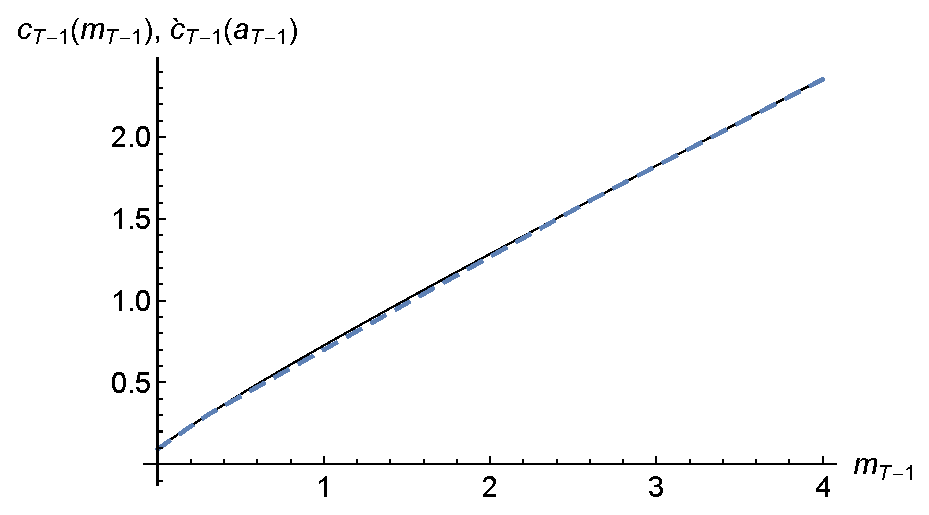
\includegraphics{./Figures/PlotComparecTm1AD}}
  \caption{$\cFunc_{T-1}({m}_{T-1})$ (solid) versus $\Alt{\cFunc}_{T-1}({m}_{T-1})$ (dashed)}
  \label{fig:ComparecTm1AD}
\end{figure}
Figure~\ref{fig:ComparecTm1AD} plots the actual consumption function
${\cFunc}_{T-1}$ and the approximated consumption function $\Alt{\cFunc}_{T-1}$
derived by the method of endogenous grid points. Compared to the approximate consumption
functions illustrated in Figure~\ref{fig:PlotcTm1ABC} $\Alt{\cFunc}_{T-1}$ is quite close
to the actual consumption function.


\ifthenelse{\boolean{MyNotes}}{\marginpar{\tiny Different transformation for $\vFunc$ than for $\vFunc^{\prime}$.}}{}

\hypertarget{Improving-the-a-Grid}{}
\subsection{Improving the $\aNrm$ Grid}

Thus far, we have arbitrarily used $\aNrm$ gridpoints of
$\{0.,1.,2.,3.,4.\}$ (augmented in the last subsection by
$\underline{a}_{T-1}$).  But it has been obvious from the figures that
the approximated $\Alt{\cFunc}_{T^{+}-1}$ function tends to be farthest from its true
value $\cFunc_{T^{+}-1}$ at low values of ${a}$.  Combining this with our insight that
$\underline{a}_{T-1}$ is a lower bound, we are now in position to
define a more deliberate method for constructing gridpoints for
${a}_{T-1}$ -- a method that yields values that are more densely
spaced than the uniform grid at low values of ${a}$.  A pragmatic
choice that works well is to find the values such that (1) the last
value \textit{exceeds the lower bound} by the same amount $\bar{a}_{T-1}$
as our original maximum gridpoint (in our case, 4.); (2) we have the
same number of gridpoints as before; and (3) the \textit{multi-exponential growth rate} (that is, $e^{e^{e^{...}}}$ for some
number of exponentiations $n_{\TranShkEmp}$) from each point to the next point is
constant (instead of, as previously, imposing constancy of the
absolute gap between points).

\hypertarget{GothVInvVSGothCEEE}{}
\begin{figure}
  \centerline{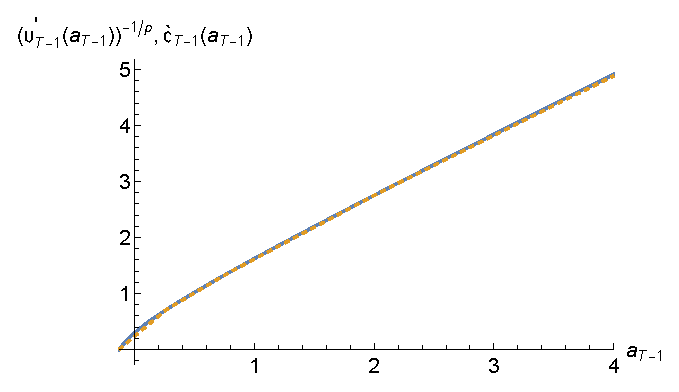
\includegraphics{./Figures/GothVInvVSGothCEEE}}
  \caption{$\cFunc_{T^{+}-1}({a}_{T-1})$ versus
    $\Alt{\cFunc}_{T^{+}-1}({a}_{T-1})$, Multi-Exponential \texttt{aVec}}
  \label{fig:GothVInvVSGothCEE}
\end{figure}


\hypertarget{GothVVSGothCInvEEE}{}
\begin{figure}
  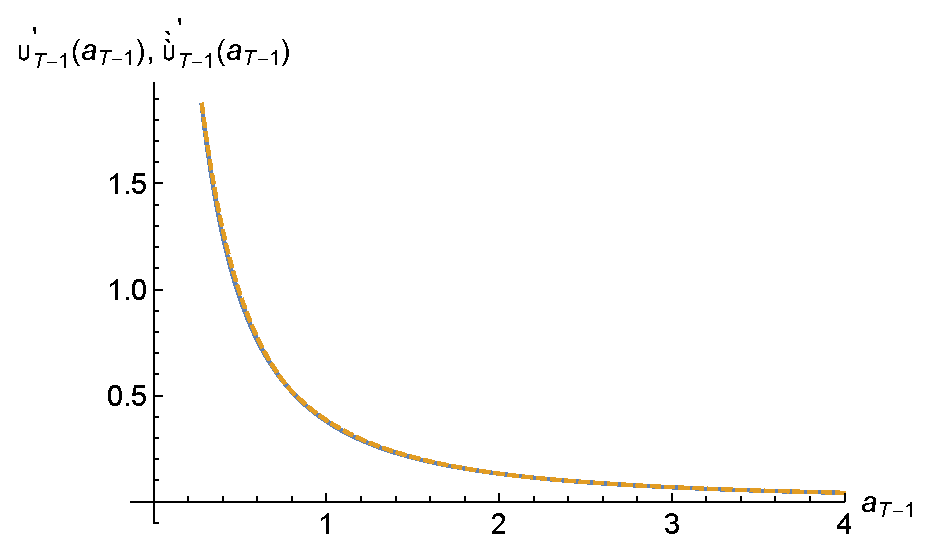
\includegraphics{./Figures/GothVVSGothCInvEEE}
  \caption{$\vFunc^{{a}}_{T^{+}-1}({a}_{T-1})$ vs.
    $\Alt{\Alt{\vFunc}}_{T^{+}-1}^{\prime}({a}_{T-1})$, Multi-Exponential \texttt{aVec}}
  \label{fig:GothVVSGothCInvEE}
\end{figure}

The results (generated by the program \texttt{2periodIntExpFOCInvEEE.m})
are depicted in Figures~\ref{fig:GothVInvVSGothCEE} and
\ref{fig:GothVVSGothCInvEE}, which are notably closer to their
respective truths than the corresponding figures that used the original
grid.

\hypertarget{The-Method-of-Moderation}{}
\subsection{The Method of Moderation}

\begin{verbatimwrite}{./cctwMoM/EndogGptsProbs.tex}

  Unfortunately, this endogenous gridpoints solution is not very
  well-behaved outside the original range of gridpoints targeted by
  the solution method.  (Though other common solution methods are no
  better outside their own predefined ranges).
  Figure~\ref{fig:ExtrapProblem} demonstrates the point by plotting
  the amount of precautionary saving implied by a linear extrapolation
  of our approximated consumption rule (the consumption of the perfect
  foresight consumer $\cFuncAbove_{T-1}$ minus our approximation to
  optimal consumption under uncertainty, $\Alt{\cFunc}_{T-1}$).
  Although theory proves that precautionary saving is always positive,
  the linearly extrapolated numerical approximation eventually
  predicts negative precautionary saving (at the point in the figure
  where the extrapolated locus crosses the horizontal axis).

  \hypertarget{ExtrapProblemPlot}{}
  \begin{figure}
    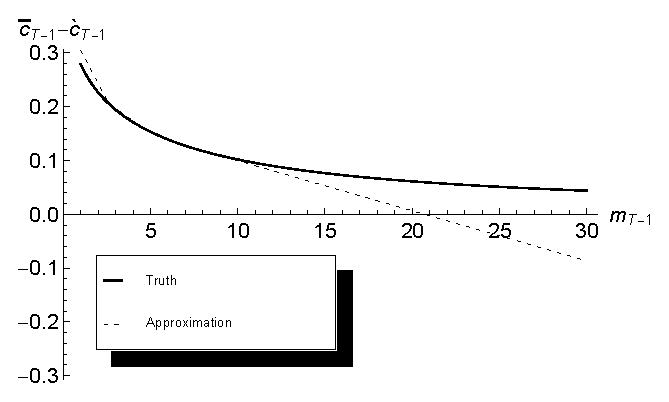
\includegraphics{./Figures/ExtrapProblemPlot}
    \caption{For Large Enough ${m}_{T-1}$, Predicted Precautionary Saving is Negative (Oops!)}
    \label{fig:ExtrapProblem}
  \end{figure}

  This error cannot be fixed by extending the upper gridpoint; in the
  presence of serious uncertainty, the consumption rule will need to be
  evaluated outside of \textit{any} prespecified grid (because starting
  from the top gridpoint, a large enough realization of the uncertain
  variable will push next period's realization of assets above that
  top; a similar argument applies below the bottom gridpoint).  While a judicious extrapolation technique can prevent this
  problem from being fatal (for example by carefully excluding negative
  precautionary saving), the problem is often dealt with using inelegant
  methods whose implications for the accuracy of the solution are
  difficult to gauge.
\end{verbatimwrite}

  Unfortunately, this endogenous gridpoints solution is not very
  well-behaved outside the original range of gridpoints targeted by
  the solution method.  (Though other common solution methods are no
  better outside their own predefined ranges).
  Figure~\ref{fig:ExtrapProblem} demonstrates the point by plotting
  the amount of precautionary saving implied by a linear extrapolation
  of our approximated consumption rule (the consumption of the perfect
  foresight consumer $\cFuncAbove_{T-1}$ minus our approximation to
  optimal consumption under uncertainty, $\Alt{\cFunc}_{T-1}$).
  Although theory proves that precautionary saving is always positive,
  the linearly extrapolated numerical approximation eventually
  predicts negative precautionary saving (at the point in the figure
  where the extrapolated locus crosses the horizontal axis).

  \hypertarget{ExtrapProblemPlot}{}
  \begin{figure}
    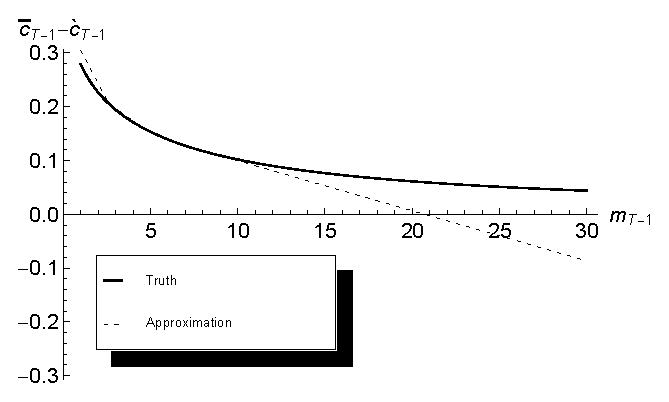
\includegraphics{./Figures/ExtrapProblemPlot}
    \caption{For Large Enough ${m}_{T-1}$, Predicted Precautionary Saving is Negative (Oops!)}
    \label{fig:ExtrapProblem}
  \end{figure}

  This error cannot be fixed by extending the upper gridpoint; in the
  presence of serious uncertainty, the consumption rule will need to be
  evaluated outside of \textit{any} prespecified grid (because starting
  from the top gridpoint, a large enough realization of the uncertain
  variable will push next period's realization of assets above that
  top; a similar argument applies below the bottom gridpoint).  While a judicious extrapolation technique can prevent this
  problem from being fatal (for example by carefully excluding negative
  precautionary saving), the problem is often dealt with using inelegant
  methods whose implications for the accuracy of the solution are
  difficult to gauge.
\unskip

\begin{verbatimwrite}{./cctwMoM/MoM-Prelims.tex}
  As a preliminary to our solution, define $\hEnd_{t}$ as
  end-of-period human wealth (the present discounted value
  of future labor income) for a perfect foresight version of the problem
  of a `risk optimist:' a consumer who believes with perfect confidence
  that the shocks will always take the value 
  \PermShkOn
  {1, $\TranShkEmp_{t+n} = \Ex[\TranShkEmp]=1~\forall~n>0$ and $\PermShk_{t+n} = \Ex[\PermShk]=1~\forall~n>0$.}
  {1, $\TranShkEmp_{t+n} = \Ex[\TranShkEmp]=1~\forall~n>0$.}
  The solution to a perfect foresight problem of this kind takes the
  form\footnote{For a derivation, see \cite{BufferStockTheory}; $\MPCmin_{t}$ is defined therein as the MPC of the perfect foresight consumer with horizon $T-t$.}
\end{verbatimwrite}
  As a preliminary to our solution, define $\hEnd_{t}$ as
  end-of-period human wealth (the present discounted value
  of future labor income) for a perfect foresight version of the problem
  of a `risk optimist:' a consumer who believes with perfect confidence
  that the shocks will always take the value
  \pShkOn
  {1, $\tShkEmp_{t+n} = \Ex[\tShkEmp]=1~\forall~n>0$ and $\pShk_{t+n} = \Ex[\pShk]=1~\forall~n>0$.}
  {1, $\tShkEmp_{t+n} = \Ex[\tShkEmp]=1~\forall~n>0$.}
  The solution to a perfect foresight problem of this kind takes the
  form\footnote{For a derivation, see \cite{BufferStockTheory}; $\MinMPC_{t}$ is defined therein as the MPC of the perfect foresight consumer with horizon $T-t$.}
\unskip
\begin{verbatimwrite}{./Equations/cFuncAbove.tex}
  \begin{equation}\begin{gathered}\begin{aligned}
        \cFuncAbove_{t}(\mNrm_{t})  & = (\mNrm_{t} + \hEnd_{t})\MPCmin_{t} \label{eq:cFuncAbove}
      \end{aligned}\end{gathered}\end{equation}
  for a constant minimal marginal propensity to consume $\MPCmin_{t}$ given below.
\end{verbatimwrite}
\begin{eqnarray}
  \cFuncAbove_{t}(\mRat_{t}) & = & (\mRat_{t} + \hEnd_{t})\MinMPC_{t} \label{eq:cFuncAbove}
\end{eqnarray}
for a constant minimal marginal propensity to consume $\MinMPC_{t}$ given below.
\unskip

\begin{verbatimwrite}{./cctwMoM/MoM-Words.tex}
  We similarly define $\hEndMin_{t}$ as `minimal human wealth,' the
  present discounted value of labor income if the shocks were to take on
  their worst possible value in every future period \PermShkOn
  {$\TranShkEmp_{t+n} = \TranShkEmpMin ~\forall~n>0$ and $\PermShk_{t+n} =
    \PermShkMin ~\forall~n>0$} {$\TranShkEmp_{t+n} = \TranShkEmpMin
    ~\forall~n>0$} (which we define as corresponding to the beliefs of a
  `pessimist').

  \ctw{}{We will call a `realist' the consumer who correctly perceives the true
    probabilities of the future risks and optimizes accordingly.}

  A first useful point is that, for the realist, a lower bound for the
  level of market resources is $\ushort{m}_{t} = -\hEndMin_{t}$, because
  if ${m}_{t}$ equalled this value then there would be a positive finite
  chance (however small) of receiving \PermShkOn
  {$\TranShkEmp_{t+n}=\TranShkEmpMin$ and $\PermShk_{t+n}=\PermShkMin$}
  {$\TranShkEmp_{t+n}=\TranShkEmpMin$}
  in
  every future period, which would require the consumer to set ${c}_{t}$
  to zero in order to guarantee that the intertemporal budget constraint
  holds\ctw{.}{~(this is the multiperiod generalization of the discussion in
    section \ref{subsec:LiqConstrSelfImposed} about
    $\ushort{a}_{T-1}$).}  Since consumption of zero yields negative
  infinite utility, the solution to realist consumer's problem is not well
  defined for values of ${m}_{t} < \ushort{m}_{t}$, and the limiting
  value of the realist's ${c}_t$ is zero as ${m}_{t} \downarrow \ushort{m}_{t}$.

  Given this result, it will be convenient to define `excess' market
  resources as the amount by which actual resources exceed the lower
  bound, and `excess' human wealth as the amount by which mean expected human wealth
  exceeds guaranteed minimum human wealth:
  \begin{equation*}\begin{gathered}\begin{aligned}
        \aboveMin \mNrm_{t}  & = {m}_{t}+\overbrace{\hEndMin_{t}}^{=-\ushort{m}_{t}}
        \\  \aboveMin \hEnd_{t}  & = \hEnd_{t}-\hEndMin_{t}.
      \end{aligned}\end{gathered}\end{equation*}

  We can now transparently define the optimal
  consumption rules for the two perfect foresight problems, those of the
  `optimist' and the `pessimist.'  The `pessimist' perceives human
  wealth to be equal to its minimum feasible value $\hEndMin_{t}$ with certainty, so 
  consumption is given by the perfect foresight solution
  \begin{equation*}\begin{gathered}\begin{aligned}
        \cFuncBelow_{t}(m_{t})  & = ({m}_{t}+\hEndMin_{t})\MPCmin_{t}
        \\  & = \aboveMin \mNrm_{t}\MPCmin_{t}
        .
      \end{aligned}\end{gathered}\end{equation*}

  The `optimist,' on the other hand, pretends that there is no uncertainty
  about future income, and therefore consumes
  \begin{equation*}\begin{gathered}\begin{aligned}
        \cFuncAbove_{t}(m_{t})  & = ({m}_{t} +\hEndMin_{t} - \hEndMin_{t} + \hEnd_{t} )\MPCmin_{t}
        \\    & = (\aboveMin \mNrm_{t} + \aboveMin \hEnd_{t})\MPCmin_{t}
        \\      & = \cFuncBelow_{t}(m_{t})+\aboveMin \hEnd_{t} \MPCmin_{t}
        .
      \end{aligned}\end{gathered}\end{equation*}

  It seems obvious that the spending of the realist will be strictly greater
  than that of the pessimist and strictly less than that of the
  optimist.  Figure~\ref{fig:IntExpFOCInvPesReaOptNeedHiPlot} illustrates the proposition for the consumption rule in period $T-1$.  
\end{verbatimwrite}
  We similarly define $\hEndMin_{t}$ as `minimal human wealth,' the
  present discounted value of labor income if the shocks were to take on
  their worst possible value in every future period \pShkOn
  {$\tShkEmp_{t+n} = \tShkEmpMin ~\forall~n>0$ and $\pShk_{t+n} =
    \pShkMin ~\forall~n>0$} {$\tShkEmp_{t+n} = \tShkEmpMin
    ~\forall~n>0$} (which we define as corresponding to the beliefs of a
  `pessimist').

  \ctw{}{We will call a `realist' the consumer who correctly perceives the true
    probabilities of the future risks and optimizes accordingly.}

  A first useful point is that, for the realist, a lower bound for the
  level of market resources is $\ushort{m}_{t} = -\hEndMin_{t}$, because
  if ${m}_{t}$ equalled this value then there would be a positive finite
  chance (however small) of receiving \pShkOn
  {$\tShkEmp_{t+n}=\tShkEmpMin$ and $\pShk_{t+n}=\pShkMin$}
  {$\tShkEmp_{t+n}=\tShkEmpMin$}
  in
  every future period, which would require the consumer to set ${c}_{t}$
  to zero in order to guarantee that the intertemporal budget constraint
  holds\ctw{.}{~(this is the multiperiod generalization of the discussion in
    section \ref{subsec:LiqConstrSelfImposed} about
    $\ushort{a}_{T-1}$).}  Since consumption of zero yields negative
  infinite utility, the solution to realist consumer's problem is not well
  defined for values of ${m}_{t} < \ushort{m}_{t}$, and the limiting
  value of the realist's ${c}_t$ is zero as ${m}_{t} \downarrow \ushort{m}_{t}$.

  Given this result, it will be convenient to define `excess' market
  resources as the amount by which actual resources exceed the lower
  bound, and `excess' human wealth as the amount by which mean expected human wealth
  exceeds guaranteed minimum human wealth:
  \begin{equation*}\begin{gathered}\begin{aligned}
    \aboveMin \mRat_{t}  & = {m}_{t}+\overbrace{\hEndMin_{t}}^{=-\ushort{m}_{t}}
    \\  \aboveMin \hEnd_{t}  & = \hEnd_{t}-\hEndMin_{t}.
  \end{aligned}\end{gathered}\end{equation*}

  We can now transparently define the optimal
  consumption rules for the two perfect foresight problems, those of the
  `optimist' and the `pessimist.'  The `pessimist' perceives human
  wealth to be equal to its minimum feasible value $\hEndMin_{t}$ with certainty, so
  consumption is given by the perfect foresight solution
  \begin{equation*}\begin{gathered}\begin{aligned}
    \cFuncBelow_{t}(m_{t})  & = ({m}_{t}+\hEndMin_{t})\MinMPC_{t}
    \\  & = \aboveMin \mRat_{t}\MinMPC_{t}
             .
  \end{aligned}\end{gathered}\end{equation*}

  The `optimist,' on the other hand, pretends that there is no uncertainty
  about future income, and therefore consumes
  \begin{equation*}\begin{gathered}\begin{aligned}
    \cFuncAbove_{t}(m_{t})  & = ({m}_{t} +\hEndMin_{t} - \hEndMin_{t} + \hEnd_{t} )\MinMPC_{t}
    \\    & = (\aboveMin \mRat_{t} + \aboveMin \hEnd_{t})\MinMPC_{t}
    \\      & = \cFuncBelow_{t}(m_{t})+\aboveMin \hEnd_{t} \MinMPC_{t}
                 .
  \end{aligned}\end{gathered}\end{equation*}

  It seems obvious that the spending of the realist will be strictly greater
  than that of the pessimist and strictly less than that of the
  optimist.  Figure~\ref{fig:IntExpFOCInvPesReaOptNeedHiPlot} illustrates the proposition for the consumption rule in period $T-1$.
\unskip
\begin{verbatimwrite}{\econtexRoot/Figures/IntExpFOCInvPesReaOptNeedHiPlot.tex}
  \hypertarget{IntExpFOCInvPesReaOptNeedHiPlot}{}
  \begin{figure}
    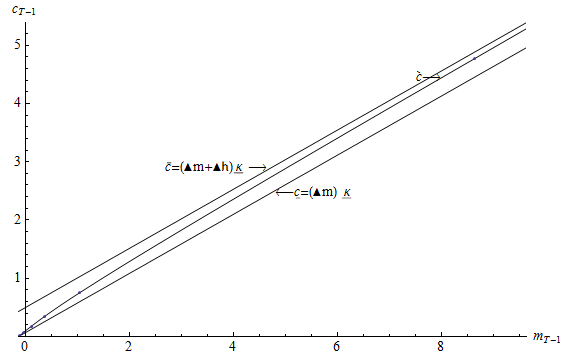
\includegraphics{./Figures/IntExpFOCInvPesReaOptNeedHiPlot}
    \caption{Moderation Illustrated: $\underline{\cFunc}_{T-1} < \Alt{\cFunc}_{T-1} < \bar{\cFunc}_{T-1}$}
    \label{fig:IntExpFOCInvPesReaOptNeedHiPlot}
  \end{figure}
\end{verbatimwrite}
  \hypertarget{IntExpFOCInvPesReaOptNeedHiPlot}{}
  \begin{figure}
    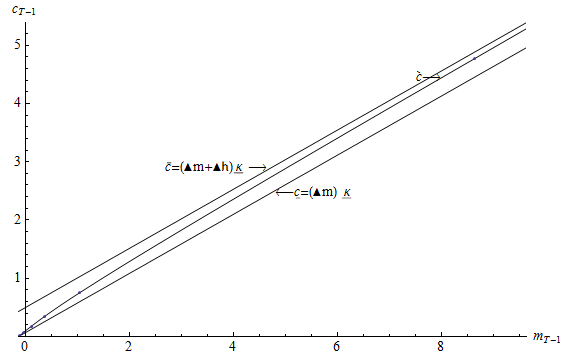
\includegraphics{./Figures/IntExpFOCInvPesReaOptNeedHiPlot}
    \caption{Moderation Illustrated: $\underline{\cFunc}_{T-1} < \Alt{\cFunc}_{T-1} < \bar{\cFunc}_{T-1}$}
    \label{fig:IntExpFOCInvPesReaOptNeedHiPlot}
  \end{figure}
\unskip
\begin{verbatimwrite}{./cctwMoM/MoM-Words-Rest.tex}

  \indent The proof is more difficult than might be imagined, but
  the necessary work is done in \cite{BufferStockTheory} so we will take
  the proposition as a fact and proceed by manipulating the inequality:
\end{verbatimwrite}

  \indent The proof is more difficult than might be imagined, but
  the necessary work is done in \cite{BufferStockTheory} so we will take
  the proposition as a fact and proceed by manipulating the inequality:
\unskip
\begin{verbatimwrite}{./Equations/MoM-Inequalities.tex}
  \begin{center}
    \begin{tabular}{rcl}
      $ \aboveMin \mNrm_{t} \MPCmin_{t} < $ & $ \cFunc_{t}(\ushort{m}_{t}+\aboveMin \mNrm_{t}) $ & $< (\aboveMin \mNrm_{t}+\aboveMin \hEnd_{t})\MPCmin_{t} $
      \\  $- \aboveMin \mNrm_{t} \MPCmin_{t} > $ & $ -\cFunc_{t}(\ushort{m}_{t}+\aboveMin \mNrm_{t}) $ & $> -(\aboveMin \mNrm_{t}+\aboveMin \hEnd_{t})\MPCmin_{t} $
      \\  $ \aboveMin \hEnd_{t} \MPCmin_{t} > $ & $ \bar{\cFunc}_{t}(\ushort{m}_{t}+\aboveMin \mNrm_{t})-\cFunc_{t}(\ushort{m}_{t}+\aboveMin \mNrm_{t}) $ & $> 0$
      \\  $1 > $ & $ \underbrace{\left(\frac{\bar{\cFunc}_{t}(\ushort{m}_{t}+\aboveMin \mNrm_{t})-\cFunc_{t}(\ushort{m}_{t}+\aboveMin \mNrm_{t})}{\aboveMin \hEnd_{t} \MPCmin_{t}}\right)}_{\equiv \Hi{\koppa}_{t}} $ & $> 0$
    \end{tabular}
  \end{center}
\end{verbatimwrite}
  \begin{center}
    \begin{tabular}{rcl}
      $ \aboveMin \mRat_{t} \MinMPC_{t} < $ & $ \cFunc_{t}(\ushort{m}_{t}+\aboveMin \mRat_{t}) $ & $< (\aboveMin \mRat_{t}+\aboveMin \hEnd_{t})\MinMPC_{t} $
      \\  $- \aboveMin \mRat_{t} \MinMPC_{t} > $ & $ -\cFunc_{t}(\ushort{m}_{t}+\aboveMin \mRat_{t}) $ & $> -(\aboveMin \mRat_{t}+\aboveMin \hEnd_{t})\MinMPC_{t} $
      \\  $ \aboveMin \hEnd_{t} \MinMPC_{t} > $ & $ \bar{\cFunc}_{t}(\ushort{m}_{t}+\aboveMin \mRat_{t})-\cFunc_{t}(\ushort{m}_{t}+\aboveMin \mRat_{t}) $ & $> 0$
      \\  $1 > $ & $ \underbrace{\left(\frac{\bar{\cFunc}_{t}(\ushort{m}_{t}+\aboveMin \mRat_{t})-\cFunc_{t}(\ushort{m}_{t}+\aboveMin \mRat_{t})}{\aboveMin \hEnd_{t} \MinMPC_{t}}\right)}_{\equiv \Hi{\koppa}_{t}} $ & $> 0$
    \end{tabular}
  \end{center}
\unskip
\begin{verbatimwrite}{./cctwMoM/MoM-Inequalities-Describe.tex}
  where the fraction in the middle of the last inequality is the ratio
  of actual precautionary saving (the numerator is the difference
  between perfect-foresight consumption and optimal consumption in the
  presence of uncertainty) to the maximum conceivable amount of
  precautionary saving (the amount that would be undertaken by the
  pessimist who consumes nothing out of any future income beyond the perfectly certain component).
\end{verbatimwrite}
  where the fraction in the middle of the last inequality is the ratio
  of actual precautionary saving (the numerator is the difference
  between perfect-foresight consumption and optimal consumption in the
  presence of uncertainty) to the maximum conceivable amount of
  precautionary saving (the amount that would be undertaken by the
  pessimist who consumes nothing out of any future income beyond the perfectly certain component).
\unskip

\begin{verbatimwrite}{./Equations/MoM-KoppaOfMu.tex}
  Defining $\mu_{t} =
  \log \aboveMin \mNrm_{t}$ (which can range from $-\infty$ to $\infty$), the object in the middle of the last inequality is
  \begin{equation}\begin{gathered}\begin{aligned}
        \Hi{\koppa}_{t}(\mu_{t})   & \equiv  \left(\frac{\bar{\cFunc}_{t}(\ushort{m}_{t}+e^{\mu_{t}})-\cFunc_{t}(\ushort{m}_{t}+e^{\mu_{t}})}{\aboveMin \hEnd_{t} \MPCmin_{t}}\right), \label{eq:koppa}
      \end{aligned}\end{gathered}\end{equation}
  and we now define
  \begin{equation}\begin{gathered}\begin{aligned}
        \Hi{\chiFunc}_{t}(\mu_{t})  & = \log \left(\frac{1-\Hi{\koppa}_{t}(\mu_{t})}{\Hi{\koppa}_{t}(\mu_{t})}\right)
        \\  & = \log \left(1/\Hi{\koppa}_{t}(\mu_{t})-1\right) \label{eq:chi}
      \end{aligned}\end{gathered}\end{equation}
\end{verbatimwrite}
Defining $\mu_{t} =
\log \aboveMin \mRat_{t}$ (which can range from $-\infty$ to $\infty$), the object in the middle of the last inequality is
\begin{eqnarray}
\Hi{\koppa}_{t}(\mu_{t})  & \equiv & \left(\frac{\bar{\cFunc}_{t}(\ushort{m}_{t}+e^{\mu_{t}})-\cFunc_{t}(\ushort{m}_{t}+e^{\mu_{t}})}{\aboveMin \hEnd_{t} \MinMPC_{t}}\right), \label{eq:koppa}
\end{eqnarray}
and we now define
\begin{eqnarray}
  \Hi{\chiFunc}_{t}(\mu_{t}) & = & \log \left(\frac{1-\Hi{\koppa}_{t}(\mu_{t})}{\Hi{\koppa}_{t}(\mu_{t})}\right)
\\ & = & \log \left(1/\Hi{\koppa}_{t}(\mu_{t})-1\right) \label{eq:chi}
\end{eqnarray}
\unskip
\begin{verbatimwrite}{./cctwMoM/MoM-KoppaOfMu-Describe.tex}
  which has the virtue that it is linear in the limit as $\mu_{t}$ approaches $+\infty$.

  Given $\Hi{\chiFunc}$, the consumption function can be recovered from
\end{verbatimwrite}
  which has the virtue that it is linear in the limit as $\mu_{t}$ approaches $+\infty$.

  Given $\Hi{\chiFunc}$, the consumption function can be recovered from
\unskip
\begin{verbatimwrite}{./Equations/cFuncHi.tex}
  \begin{equation}\begin{gathered}\begin{aligned}
        \Hi{\cFunc}_{t}  & = \bar{\cFunc}_{t}-\overbrace{\left(\frac{1}{1+\exp(\Hi{\chiFunc}_{t})}\right)}^{=\Hi{\koppa}_{t}} \aboveMin \hEnd_{t} \MPCmin_{t}. \label{eq:cFuncHi}
      \end{aligned}\end{gathered}\end{equation}
\end{verbatimwrite}
\begin{eqnarray}
  \Hi{\cFunc}_{t} & = & \bar{\cFunc}_{t}-\overbrace{\left(\frac{1}{1+\exp(\Hi{\chiFunc}_{t})}\right)}^{=\Hi{\koppa}_{t}} \aboveMin \hEnd_{t} \MinMPC_{t}. \label{eq:cFuncHi}
\end{eqnarray}
\unskip

\begin{verbatimwrite}{./cctwMoM/MoM-End.tex}

  Thus, the procedure is to calculate $\Hi{\chiFunc}_{t}$ at the points
  $\vec{\mu}_{t}$ corresponding to the log of the $\aboveMin
  \vec{m}_{t}$ points defined above, and then using these to construct an
  interpolating approximation $\Alt{\Hi{\chiFunc}}_{t}$ from which we indirectly obtain our 
  approximated consumption rule $\Alt{\Hi{\cFunc}}_{t}$ by substituting $\Alt{\Hi{\chiFunc}}_{t}$ for $\Hi{\chiFunc}$ in equation \eqref{eq:cFuncHi}.

  Because this method relies upon the fact that the problem is easy to
  solve if the decision maker has unreasonable views (either in the
  optimistic or the pessimistic direction), and because the correct
  solution is always between these immoderate extremes, we call our 
  solution procedure the `method of moderation.'

  Results are shown in Figure~\ref{fig:ExtrapProblemSolved}; a reader
  with very good eyesight might be able to detect the barest hint of a
  discrepancy between the Truth and the Approximation at the far
  righthand edge of the figure\ctw{.}{ -- a stark contrast with the calamitous
    divergence evident in Figure~\ref{fig:ExtrapProblem}.}{}
  \hypertarget{ExtrapProblemSolvedPlot}{}
  \begin{figure}
    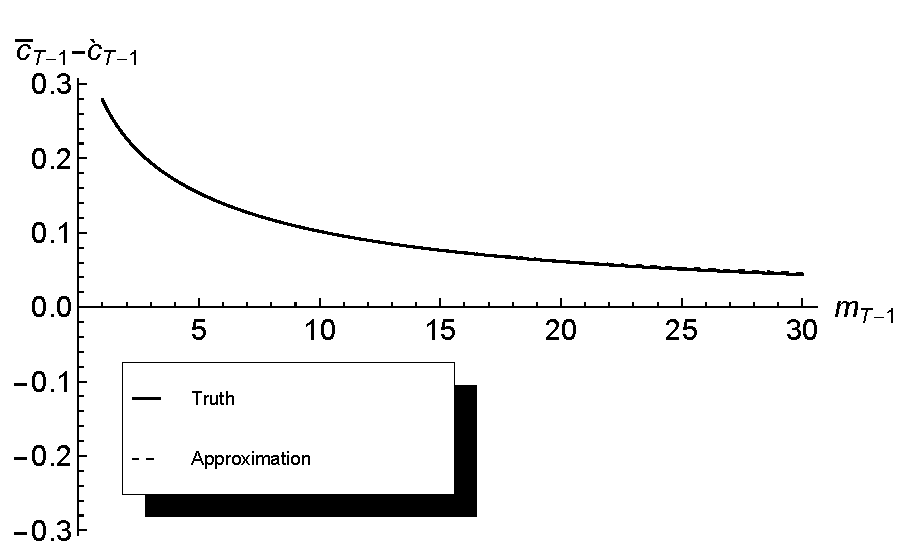
\includegraphics{./Figures/ExtrapProblemSolvedPlot}
    \caption{Extrapolated $\Alt{\Hi{\cFunc}}_{T-1}$ Constructed Using the Method of Moderation}
    \label{fig:ExtrapProblemSolved}
  \end{figure}
\end{verbatimwrite}

  Using these inequalities, we now construct another approximation of consumption function, $\tilde{\cFunc}_{t}({m}_{t})$, whose performance is better for points lying outside the original grid. Denote the largest and smallest points on that grid by $\bar{m}$ and $\underaccent{\bar}{m}$ respectively.  The above inequality then tells us that we have a limiting function $ \bar{\cFunc}_{t}(\ushort{m}_{t}+\aboveMin \mNrm_{t})$ for values of m, greater than $\bar{m}$, i.e., for values of $m_t > \bar{m} $  and $m_t \rightarrow \infty $, the behavior of $\tilde{\cFunc}_{t}({m}_{t})$ is anchored by $ \bar{\cFunc}_{t}({m}_{t})$. More precisely, our improved consumption function's behavior would be governed by following  rules:
\begin{itemize}
\item $\tilde{\cFunc}_{t}({m}_{t})$  = $ \cFunc_{t}({m}_{t})$ when $m_t$ falls inside the specified grid, i.e.\ when $m_t$ < $\bar{m}$
\item $\tilde{\cFunc}_{t}({m}_{t})  \rightarrow    \cFuncBelow_{t}(m_{t})  $  as $m_t \rightarrow 0$.
\item $\tilde{\cFunc}_{t}({m}_{t})  \rightarrow   \bar{\cFunc}_{t}({m}_{t}) $  as $m_t \rightarrow \infty$.
\end{itemize}

With the above principle in mind, start with a point $m$ beyond the specified grid, $m > \bar{m}$. Since the gridpoints in our case are one-dimensional, the point in the grid closest to $m$ is $\bar{m}$. This method first calculates a standardized distance between $m$ and $\bar{m}$ as:
\begin{align*}
  d(m, \bar{m}) & =  \left| \frac{m - \bar{m}}{\bar{m}} \right|
\end{align*}
and uses it to compute the combination between extrapolated value  $ \cFunc_{t}({m}_{t})$ and the limit-value $\bar{\cFunc}_{t}({m}_{t}) $ as :

\[  \tilde{\cFunc}_{t}({m}_{t}) = e^{-d(m, \bar{m})} \times   \cFunc_{t}({m}_{t})  +  (1-e^{-d(m, \bar{m})})\times  \bar{\cFunc}_{t}({m}_{t})\]

i.e. our improved approximation of consumption function is a weighted average of  $ \cFunc_{t}({m}_{t})$ and  $\bar{\cFunc}_{t}({m}_{t}) $. As the distance between $m$ and $\bar{m}$ grows,  $\bar{\cFunc}_{t}({m}_{t})$ is given more weight. That makes intuitive sense as $m$ being far outside the pre-specified grid point range corresponds to the case of a large realization of temporary shock. And that means, consumer would have enormous market resources at its disposal than usual, in which case its consumption behavior would closely follow that of an optimist (i.e. $\bar{\cFunc}_{t}({m}_{t})$).
Readers interested in alternative methods of extrapolation should refer this HARK \href{https://github.com/econ-ark/HARK/blob/master/examples/Interpolation/DecayInterp.ipynb}{documentation}.

So far, we have discussed the procedure to carry out extrapolation when the point is larger than the maximum grid point that was specified with $\bar{\cFunc}(m)$ as the benchmark function. By similar reasoning, we can also conduct extrapolation when the point is smaller than the minimum grid point with  $\cFuncBelow(m)$ serving now as the benchmark function anchoring the behavior of approximate consumption function in that point range.


  Because this method relies upon the fact that the problem is easy to
  solve if the decision maker has unreasonable views (either in the
  optimistic or the pessimistic direction), and because the correct
  solution is always between these immoderate extremes, we call our
  solution procedure the `method of moderation.'

  Results are shown in Figure~\ref{fig:ExtrapProblemSolved}; a reader
  with very good eyesight might be able to detect the barest hint of a
  discrepancy between the Truth and the Approximation at the far
  righthand edge of the figure\ctw{.}{ -- a stark contrast with the calamitous
    divergence evident in Figure~\ref{fig:ExtrapProblem}.}{}
  \hypertarget{ExtrapProblemSolvedPlot}{}
  \begin{figure}
    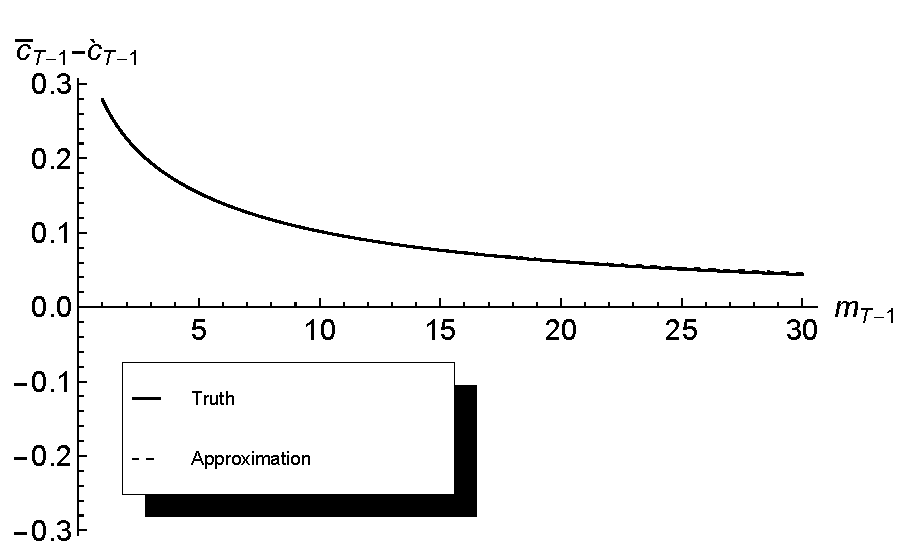
\includegraphics{./Figures/ExtrapProblemSolvedPlot}
    \caption{Extrapolated $\Alt{\Hi{\cFunc}}_{T-1}$ Constructed Using the Method of Moderation}
    \label{fig:ExtrapProblemSolved}
  \end{figure}

\unskip

\hypertarget{Approximating-the-Slope-Too}{}
\subsection{Approximating the Slope Too}


Until now, we have calculated the level of consumption at
various different gridpoints and used linear interpolation\ctw{.}{ (either
  directly for $\cFunc_{T-1}$ or indirectly for, say, $\Hi{\chiFunc}_{T-1}$).}  But the
resulting piecewise linear approximations have the unattractive feature
that they are not differentiable at the `kink points' that correspond to
the gridpoints where the slope of the function changes discretely.



\cite{BufferStockTheory} shows that the true consumption function for
this problem 
is `smooth:' It
exhibits a well-defined unique marginal propensity to consume at every
positive value of ${m}$.  This suggests that we should calculate, not
just the level of consumption, but also the marginal propensity to
consume (henceforth $\MPC$) at each gridpoint, and then find an
interpolating approximation that smoothly matches both the level and the slope
at those points.

This requires us to differentiate \eqref{eq:koppa} and \eqref{eq:chi}, yielding
\begin{equation}\begin{gathered}\begin{aligned}
      \Hi{\koppa}_{t}^{\mu}(\mu_{t})   & = (\aboveMin \hEnd_{t} \MPCmin_{t})^{-1}e^{\mu_{t}}\left(\MPCmin_{t}-\overbrace{\cFunc^{\mNrm}_{t}(\ushort{m}_{t}+e^{\mu_{t}})}^{\equiv \MPCFunc_{t}(\mNrm_{t})}\right)  \label{eq:koppaPrime}
      \\ \Hi{\chiFunc}_{t}^{\mu}(\mu_{t})  & = \left(\frac{-\Hi{\koppa}_{t}^{\mu}(\mu_{t})/\Hi{\koppa}_{t}^{2}}{1/\Hi{\koppa}_{t}(\mu_{t})-1}\right)
    \end{aligned}\end{gathered}\end{equation}
and (dropping arguments) with some algebra these can be combined to yield
\begin{equation}\begin{gathered}\begin{aligned}
      \Hi{\chiFunc}_{t}^{\mu}  & = \left(\frac{\MPCmin_{t} \aboveMin \mNrm_{t} \aboveMin \hEnd_{t} (\MPCmin_{t}-\MPC_{t})}
        {(\cFuncAbove_{t}-\cFunc_{t})(\cFuncAbove_{t}-\cFunc_{t} - \MPCmin_{t} \aboveMin \hEnd_{t})}\right).
    \end{aligned}\end{gathered}\end{equation}

To compute the vector of values of \eqref{eq:koppaPrime} corresponding
to the points in $\vec{\mu}_{t}$, we need the marginal propensities to
consume (designated $\MPC$) at each of the gridpoints,
$\cFunc^{\mNrm}_{t}$ (the vector of such values is 
$\vec{\MPC}_{t}$).  These can be obtained by differentiating the
Euler equation \eqref{eq:upEqbetaOp} (where we define
$\mathfrak{m}_{t}({a}) \equiv \cEndStget({a})+{a}$):
\begin{equation}\begin{gathered}\begin{aligned}
      \uFunc^{{c}}({\cFunc}_{t})   & = \hat{\vEndStget}^{\aNrm}(\mathfrak{m}_{t}-{\cFunc}_{t})
    \end{aligned}\end{gathered}\end{equation}
with respect to $\aNrm$, yielding a marginal propensity to
\textit{have consumed} $\cFunc_{\overline{t}}^{\aNrm}$ at each gridpoint:
\begin{equation}\begin{gathered}\begin{aligned}
      \uPP(\cEndStget)\cEndStget^{\aNrm}  & = \hat{\vEndStget}^{\aNrm}(\mathfrak{m}_{t}-{\cFunc}_{t})
      \\ \cEndStget^{\aNrm}  & = \hat{\vEndStget}^{\aNrm}(\mathfrak{m}_{t}-{\cFunc}_{t})/\uPP(\cEndStget)
    \end{aligned}\end{gathered}\end{equation}
and the marginal propensity to consume at the beginning of the period is obtained from the marginal
propensity to have consumed by noting that
\begin{equation*}\begin{gathered}\begin{aligned}
      \cEndFunc  & = \mathfrak{m}-\aNrm
      \\ \cEndFunc^{\aNrm}+1  & = \mathfrak{m}^{\aNrm}
    \end{aligned}\end{gathered}\end{equation*}
which, together with the chain rule $\cEndFunc^{\aNrm}  = \cFunc^{\mNrm}\mathfrak{m}^{\aNrm}$,
yields the MPC from
\begin{equation}\begin{gathered}\begin{aligned}
      \cFunc^{\mNrm}(\overbrace{\cEndFunc^{\aNrm}+1}^{=\mathfrak{m}^{\aNrm}})  & = \cEndFunc^{\aNrm}
      \\ \cFunc^{\mNrm}  & = \cEndFunc^{\aNrm}/(1+\cEndFunc^{\aNrm}) \label{eq:MPCfromMPTHC}.
    \end{aligned}\end{gathered}\end{equation}


Designating $\Alt{\Hi{\cFunc}}_{T-1}$ as the approximated consumption rule obtained using an interpolating polynomial approximation to $\Hi{\chiFunc}$ that matches both the level and the first derivative at the gridpoints, Figure~\ref{fig:IntExpFOCInvPesReaOptGapPlot} plots the difference between this latest approximation and the true consumption rule for period $T-1$ up to the same large value (far beyond the largest gridpoint) used in prior figures.  Of course, at the gridpoints the approximation will match the true function; but this figure illustrates that the approximation is quite accurate far beyond the last gridpoint (which is the last point at which the difference touches the horizontal axis).  (We plot here the difference between the two functions rather than the level plotted in previous figures, because in levels the approximation error would not be detectable even to the most eagle-eyed reader.)



\hypertarget{IntExpFOCInvPesReaOptGapPlot}{}
\begin{figure}
  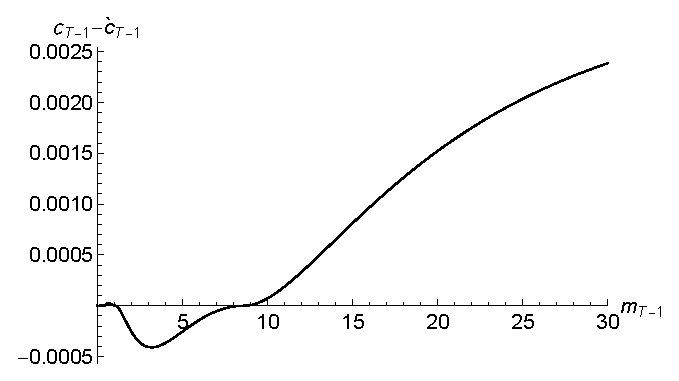
\includegraphics{./Figures/IntExpFOCInvPesReaOptGapPlot}
  \caption{Difference Between True $\cFunc_{T-1}$ and $\Alt{\Hi{\cFunc}}_{T-1}$ Is Minuscule}
  \label{fig:IntExpFOCInvPesReaOptGapPlot}
\end{figure}




\hypertarget{Value}{}
\subsection{Value}

\begin{verbatimwrite}{./cctwMoM/value-Intro.tex}

  Often it is useful to know the value function as well as the consumption rule.  Fortunately, many of the tricks used when solving for the consumption rule have a direct analogue in approximation of the value function.

  Consider the perfect foresight (or ``optimist's'') problem in period $T-1$:
  \begin{equation*}\begin{gathered}\begin{aligned}
        \bar{\vFunc}_{T-1}({m}_{T-1})  & \equiv  \uFunc(\cNrm_{T-1})+\DiscFac \uFunc(\cNrm_{T})
        \\  & = \uFunc(\cNrm_{T-1})\left(1+\DiscFac ((\DiscFac_{T}\Rfree)^{1/\CRRA})^{1-\CRRA}\right)
        \\  & = \uFunc(\cNrm_{T-1})\left(1+\DiscFac (\DiscFac_{T}\Rfree)^{1/\CRRA-1}\right)
        \\  & = \uFunc(\cNrm_{T-1})\left(1+(\DiscFac_{T}\Rfree)^{1/\CRRA}/\Rfree\right)
        \\  & = \uFunc(\cNrm_{T-1})\underbrace{\mbox{PDV}_{t}^{T}(\cNrm)/\cNrm_{T-1}}_{\equiv \mathbb{C}_{t}^{T}}
      \end{aligned}\end{gathered}\end{equation*}
  where $\mathbb{C}_{t}^{T}=\mbox{PDV}_{t}^{T}(\cNrm)$ is the present discounted value of consumption.
  A similar function can be constructed recursively for earlier periods, yielding
  the general expression \hypertarget{vFuncPF}{}
\end{verbatimwrite}

  Although section~\ref{subsec:vVsuP} argued that our problem is more
  efficiently solved by constructing the consumption rule than by
  approximating the value function, often it is useful to know the
  value function as well as the consumption rule.  Fortunately, many
  of the tricks used when solving for the consumption rule have a
  direct analogue in approximation of the value function.

  Consider the perfect foresight (or ``optimist's'') problem in period $T-1$:
  \begin{eqnarray*}
    \bar{\vFunc}_{T-1}({m}_{T-1}) & \equiv & \util(\cRat_{T-1})+\Discount \util(\cRat_{T})
    \\ & = & \util(\cRat_{T-1})\left(1+\Discount ((\Discount_{T}\Rfree)^{1/\CRRA})^{1-\CRRA}\right)
    \\ & = & \util(\cRat_{T-1})\left(1+\Discount (\Discount_{T}\Rfree)^{1/\CRRA-1}\right)
    \\ & = & \util(\cRat_{T-1})\left(1+(\Discount_{T}\Rfree)^{1/\CRRA}/\Rfree\right)
    \\ & = & \util(\cRat_{T-1})\underbrace{\mbox{PDV}_{t}^{T}(\cRat)/\cRat_{T-1}}_{\equiv \mathbb{C}_{t}^{T}}
  \end{eqnarray*}
  where $\mathbb{C}_{t}^{T}=\mbox{PDV}_{t}^{T}(\cRat)$ is the present discounted value of consumption.
  A similar function can be constructed recursively for earlier periods, yielding
  the general expression \hypertarget{vFuncPF}{}
\unskip
\begin{verbatimwrite}{./Equations/vFuncPF.tex}
  \begin{equation}\begin{gathered}\begin{aligned}
        \bar{\vFunc}_{t}({m}_{t})  & = \uFunc(\bar{\cNrm}_{t})\mathbb{C}_{t}^{T}\label{eq:vFuncPF}
        \\  & = \uFunc(\bar{c}_{t}) \MPCmin_{t}^{-1} % 20190820
        \\  & = \uFunc((\aboveMin \mNrm_{t}+\aboveMin \hEnd_{t})\MPCmin_{t}) \MPCmin_{t}^{-1} % 20190820
        \\  & = \uFunc(\aboveMin \mNrm_{t}+\aboveMin \hEnd_{t})\MPCmin_{t}^{1-\CRRA} \MPCmin_{t}^{-1} % 20190820
        \\  & = \uFunc(\aboveMin \mNrm_{t}+\aboveMin \hEnd_{t})\MPCmin_{t}^{-\CRRA}  % 20190820
      \end{aligned}\end{gathered}\end{equation}
  where the second line uses the fact demonstrated in \cite{BufferStockTheory} that $\mathbb{C}_{t}=\MPC^{-1}_{t}$. % 20190820

  This can be transformed as
  \begin{equation*}\begin{gathered}\begin{aligned}
        \bar{\vInv}_{t}  & \equiv  \left((1-\CRRA)\bar{\vFunc}_{t}\right)^{1/(1-\CRRA)}
        \\  & = \cNrm_{t}(\mathbb{C}_{t}^{T})^{1/(1-\CRRA)}
        \\  & = (\aboveMin \mNrm_{t}+\aboveMin \hEnd_{t})\MPCmin_{t}^{-\CRRA/(1-\CRRA)}   % 20190820
      \end{aligned}\end{gathered}\end{equation*}
\end{verbatimwrite}
  \begin{equation}\begin{gathered}\begin{aligned}
    \bar{\vFunc}_{t}({m}_{t})  & = \util(\bar{\cRat}_{t})\mathbb{C}_{t}^{T}\label{eq:vFuncPF}
    \\  & = \util(\bar{c}_{t}) \MinMPC_{t}^{-1} % 20190820
    \\  & = \util((\aboveMin \mRat_{t}+\aboveMin \hEnd_{t})\MinMPC_{t}) \MinMPC_{t}^{-1} % 20190820
    \\  & = \util(\aboveMin \mRat_{t}+\aboveMin \hEnd_{t})\MinMPC_{t}^{1-\CRRA} \MinMPC_{t}^{-1} % 20190820
    \\  & = \util(\aboveMin \mRat_{t}+\aboveMin \hEnd_{t})\MinMPC_{t}^{-\CRRA}  % 20190820
  \end{aligned}\end{gathered}\end{equation}
  where the second line uses the fact demonstrated in \cite{BufferStockTheory} that $\mathbb{C}_{t}=\MPC^{-1}_{t}$. % 20190820

  This can be transformed as
  \begin{equation*}\begin{gathered}\begin{aligned}
    \bar{\vInv}_{t}  & \equiv  \left((1-\CRRA)\bar{\vFunc}_{t}\right)^{1/(1-\CRRA)}
    \\  & = \cRat_{t}(\mathbb{C}_{t}^{T})^{1/(1-\CRRA)}
    \\  & = (\aboveMin \mRat_{t}+\aboveMin \hEnd_{t})\MinMPC_{t}^{-\CRRA/(1-\CRRA)}   % 20190820
  \end{aligned}\end{gathered}\end{equation*}
\unskip
\begin{verbatimwrite}{./cctwMoM/value-Rest.tex}
  \MPCMatch{with derivative
    \begin{equation*}\begin{gathered}\begin{aligned}
          \bar{\vInv}_{t}^{m}  & = (\mathbb{C}_{t}^{T})^{1/(1-\CRRA)}\MPCmin_{t},
          \\  & = \MPCmin_{t}^{-\CRRA/(1-\CRRA)} % 20190820
        \end{aligned}\end{gathered}\end{equation*}}{}
  and since $\mathbb{C}_{t}^{T}$ is a constant while the consumption
  function is linear, $\bar{\vInv}_{t}$ will also be linear.

  We apply the same transformation to the value function for the problem with uncertainty (the ``realist's'' problem)\MPCMatch{ and differentiate}:
  \begin{equation*}\begin{gathered}\begin{aligned}
        \bar{\vInv}_{t}  & = \left((1-\CRRA)\bar{\vFunc}_{t}({m}_{t})\right)^{1/(1-\CRRA)}
        \MPCMatch{\\ \bar{\vInv}^{m}_{t}  & = \left((1-\CRRA)\bar{\vFunc}_{t}({m}_{t})\right)^{-1+1/(1-\CRRA)}\bar{\vFunc}_{t}^{m}({m}_{t})}{}
      \end{aligned}\end{gathered}\end{equation*}
  and an excellent approximation to the value function can be obtained by
  calculating the values of $\bar{\vInv}$ at the same gridpoints used by the
  consumption function approximation, and interpolating among those points.

  However, as with the consumption approximation, we can do even better if we
  realize that the $\bar{\vInv}$ function for the optimist's problem is
  an upper bound for the ${\vInv}$ function in the presence of uncertainty, and the value function
  for the pessimist is a lower bound. Analogously to \eqref{eq:koppa}, define an upper-case
  \begin{equation}\begin{gathered}\begin{aligned}
        \hat{\Koppa}_{t}(\mu_{t})   & = \left(\frac{\bar{\vInv}_{t}(\ushort{m}_{t}+e^{\mu_{t}})-\vInv_{t}(\ushort{m}_{t}+e^{\mu_{t}})}{\aboveMin \hEnd_{t} \MPCmin_{t} (\mathbb{C}_{t}^{T})^{1/(1-\CRRA)}}\right) \label{eq:Koppa}
      \end{aligned}\end{gathered}\end{equation}
  \MPCMatch{with derivative (dropping arguments)
    \begin{equation}\begin{gathered}\begin{aligned}
          \hat{\Koppa}_{t}^{\mu}   & = (\aboveMin \hEnd_{t} \MPCmin_{t} (\mathbb{C}_{t}^{T})^{1/(1-\CRRA)})^{-1}e^{\mu_{t}}\left(\bar{\vInv}^{m}_{t}-\vInv^{m}_{t}\right) \label{eq:KoppaPrime}
          % \\  & =  (\aboveMin \hEnd_{t} \MPCmin_{t})^{-1}e^{\mu_{t}}\left((\mathbb{C}_{t}^{T})^{1/(1-\CRRA)}\MPCmin_{t}-\left((1-\CRRA)\vFunc_{t}({m}_{t})\right)^{-1+1/(1-\CRRA)}\vFunc_{t}^{m}({m}_{t})\right)  \notag
        \end{aligned}\end{gathered}\end{equation}}{}
  and an upper-case version of the $\chiFunc$ equation in \eqref{eq:chi}:
  \begin{equation}\begin{gathered}\begin{aligned}
        \hat{\Chi}_{t}(\mu_{t})  & = \log \left(\frac{1-\hat{\Koppa}_{t}(\mu_{t})}{\hat{\Koppa}_{t}(\mu_{t})}\right)
        \\  & = \log \left(1/\hat{\Koppa}_{t}(\mu_{t})-1\right) \label{eq:Chi}
      \end{aligned}\end{gathered}\end{equation}
  \MPCMatch{with corresponding derivative
    \begin{equation}\begin{gathered}\begin{aligned}
          \hat{\Chi}_{t}^{\mu}  & = \left(\frac{-\hat{\Koppa}_{t}^{\mu}/\hat{\Koppa}_{t}^{2}}{1/\hat{\Koppa}_{t}-1}\right)
        \end{aligned}\end{gathered}\end{equation}}{}
  and if we approximate these objects then invert them (as above with
  the $\Hi{\koppa}$ and $\Hi{\chiFunc}$ functions) we obtain a very high-quality
  approximation to our inverted value function at the same points for
  which we have our approximated value function:
  \begin{equation}\begin{gathered}\begin{aligned}
        \hat{\vInv}_{t}  & = \bar{\vInv}_{t}-\overbrace{\left(\frac{1}{1+\exp(\hat{\Chi}_{t})}\right)}^{=\hat{\Koppa}_{t}} \aboveMin \hEnd_{t} \MPCmin_{t} (\mathbb{C}_{t}^{T})^{1/(1-\CRRA) }
      \end{aligned}\end{gathered}\end{equation}
  from which we obtain our approximation to the value function\MPCMatch{ and its derivatives~}~as \hypertarget{vHatFunc}{}
  \begin{equation}\begin{gathered}\begin{aligned}
        \hat{\vFunc}_{t}  & = \uFunc(\hat{\vInv}_{t})
        \\  \hat{\vFunc}^{m}_{t}  & = \uFunc^{{c}}(\hat{\vInv}_{t}) \hat{\vInv}^{m}
        \MPCMatch{\\  \hat{\vFunc}^{mm}_{t}  & = \uFunc^{{c}{c}}(\hat{\vInv}_{t}) (\hat{\vInv}^{m})^{2} + \uFunc^{{c}}(\hat{\vInv}_{t})\hat{\vInv}^{mm}}{}
.
      \end{aligned}\end{gathered}\end{equation}

  Although a linear interpolation that matches the level of $\vInv$ at
  the gridpoints is simple, a Hermite interpolation that matches both
  the level and the derivative of the $\bar{\vInv}_{t}$ function at the
  gridpoints has the considerable virtue that the $\bar{\vFunc}_{t}$ derived from it numerically satisfies
  the envelope theorem at each of the gridpoints for which the problem
  has been solved.

  \MPCMatch{If we use the double-derivative calculated above to produce a higher-order Hermite polynomial, our approximation will also match
    marginal propensity to consume at the gridpoints; this would
    guarantee that the consumption function generated from the value
    function would match both the level of consumption and the
    marginal propensity to consume at the gridpoints; the numerical
    differences between the newly constructed consumption function and
    the highly accurate one constructed earlier would be negligible
    within the grid.}{}

\end{verbatimwrite}
\MPCMatch{with derivative
\begin{eqnarray*}
  \bar{\vInv}_{t}^{m} & = & (\mathbb{C}_{t}^{T})^{1/(1-\CRRA)}\MinMPC_{t},
\\ & = & \MinMPC_{t}^{-\CRRA/(1-\CRRA)} % 20190820
\end{eqnarray*}}{}
and since $\mathbb{C}_{t}^{T}$ is a constant while the consumption
function is linear, $\bar{\vInv}_{t}$ will also be linear.

We apply the same transformation to the value function for the problem with uncertainty (the ``realist's'' problem)\MPCMatch{ and differentiate}:
\begin{eqnarray*}
  \bar{\vInv}_{t} & = & \left((1-\CRRA)\bar{\vFunc}_{t}({m}_{t})\right)^{1/(1-\CRRA)}
\MPCMatch{\\ \bar{\vInv}^{m}_{t} & = & \left((1-\CRRA)\bar{\vFunc}_{t}({m}_{t})\right)^{-1+1/(1-\CRRA)}\bar{\vFunc}_{t}^{m}({m}_{t})}{}
\end{eqnarray*}
and an excellent approximation to the value function can be obtained by
calculating the values of $\bar{\vInv}$ at the same gridpoints used by the
consumption function approximation, and interpolating among those points.

However, as with the consumption approximation, we can do even better if we
realize that the $\bar{\vInv}$ function for the optimist's problem is
an upper bound for the ${\vInv}$ function in the presence of uncertainty, and the value function
for the pessimist is a lower bound. Analogously to \eqref{eq:koppa}, define an upper-case
\begin{eqnarray}
\hat{\Koppa}_{t}(\mu_{t})  & = & \left(\frac{\bar{\vInv}_{t}(\ushort{m}_{t}+e^{\mu_{t}})-\vInv_{t}(\ushort{m}_{t}+e^{\mu_{t}})}{\aboveMin \hEnd_{t} \MinMPC_{t} (\mathbb{C}_{t}^{T})^{1/(1-\CRRA)}}\right) \label{eq:Koppa}
\end{eqnarray}
\MPCMatch{with derivative (dropping arguments)
\begin{eqnarray}
 \hat{\Koppa}_{t}^{\mu}  & = & (\aboveMin \hEnd_{t} \MinMPC_{t} (\mathbb{C}_{t}^{T})^{1/(1-\CRRA)})^{-1}e^{\mu_{t}}\left(\bar{\vInv}^{m}_{t}-\vInv^{m}_{t}\right) \label{eq:KoppaPrime}
%\\ & = &  (\aboveMin \hEnd_{t} \MinMPC_{t})^{-1}e^{\mu_{t}}\left((\mathbb{C}_{t}^{T})^{1/(1-\CRRA)}\MinMPC_{t}-\left((1-\CRRA)\vFunc_{t}({m}_{t})\right)^{-1+1/(1-\CRRA)}\vFunc_{t}^{m}({m}_{t})\right)  \notag
\end{eqnarray}}{}
and an upper-case version of the $\chiFunc$ equation in \eqref{eq:chi}:
\begin{eqnarray}
  \hat{\Chi}_{t}(\mu_{t}) & = & \log \left(\frac{1-\hat{\Koppa}_{t}(\mu_{t})}{\hat{\Koppa}_{t}(\mu_{t})}\right)
\\ & = & \log \left(1/\hat{\Koppa}_{t}(\mu_{t})-1\right) \label{eq:Chi}
\end{eqnarray}
\MPCMatch{with corresponding derivative
\begin{eqnarray}
 \hat{\Chi}_{t}^{\mu} & = & \left(\frac{-\hat{\Koppa}_{t}^{\mu}/\hat{\Koppa}_{t}^{2}}{1/\hat{\Koppa}_{t}-1}\right)
\end{eqnarray}}{}
and if we approximate these objects then invert them (as above with
the $\Hi{\koppa}$ and $\Hi{\chiFunc}$ functions) we obtain a very high-quality
approximation to our inverted value function at the same points for
which we have our approximated value function:
\begin{eqnarray}
  \hat{\vInv}_{t} & = & \bar{\vInv}_{t}-\overbrace{\left(\frac{1}{1+\exp(\hat{\Chi}_{t})}\right)}^{=\hat{\Koppa}_{t}} \aboveMin \hEnd_{t} \MinMPC_{t} (\mathbb{C}_{t}^{T})^{1/(1-\CRRA) }
\end{eqnarray}
from which we obtain our approximation to the value function\MPCMatch{ and its derivatives~}~as \hypertarget{vHatFunc}{}
\begin{eqnarray*}
    \hat{\vFunc}_{t} & = & \util(\hat{\vInv}_{t})
\\  \hat{\vFunc}^{m}_{t} & = & \util^{\prime}(\hat{\vInv}_{t}) \hat{\vInv}^{m}
\MPCMatch{\\  \hat{\vFunc}^{mm}_{t} & = & \util^{\prime\prime}(\hat{\vInv}_{t}) (\hat{\vInv}^{m})^{2} + \util^{\prime}(\hat{\vInv}_{t})\hat{\vInv}^{mm}}{}
.
\end{eqnarray*}

Although a linear interpolation that matches the level of $\vInv$ at
the gridpoints is simple, a Hermite interpolation that matches both
the level and the derivative of the $\bar{\vInv}_{t}$ function at the
gridpoints has the considerable virtue that the $\bar{\vFunc}_{t}$ derived from it numerically satisfies
the envelope theorem at each of the gridpoints for which the problem
has been solved.

\MPCMatch{If we use the double-derivative calculated above to produce a higher-order Hermite polynomial, our approximation will also match
  marginal propensity to consume at the gridpoints; this would
  guarantee that the consumption function generated from the value
  function would match both the level of consumption and the
  marginal propensity to consume at the gridpoints; the numerical
  differences between the newly constructed consumption function and
  the highly accurate one constructed earlier would be negligible
  within the grid.}{}

\unskip

\hypertarget{Refinement-A-Tighter-Upper-Bound}{}
\subsection{Refinement: A Tighter Upper Bound}
\begin{verbatimwrite}{./cctwMoM/Tighter.tex}
  \cite{BufferStockTheory} derives an upper limit  $\MPCmax_{t}$ for the MPC as $m_{t}$
  approaches its lower bound.  Using this 
  fact plus the strict concavity of the consumption function yields the
  proposition that 
  \begin{equation}\begin{gathered}\begin{aligned}
        \cFunc_{t}(\ushort{m}_{t}+\aboveMin \mNrm_{t}) & < \MPCmax_{t} \aboveMin \mNrm_{t}.
      \end{aligned}\end{gathered}\end{equation}

  The solution method described above does not guarantee that
  approximated consumption will respect this constraint between gridpoints, and a failure to 
  respect the constraint can occasionally cause computational problems in solving
  or simulating the model.  Here, we 
  describe a method for constructing an approximation that always
  satisfies the constraint.

  \begin{comment} % Old text needs to be revised or eliminated
    That is, the realist's consumption function is bounded from above by both
    the \textit{unconstrained} optimist's problem already treated, as well as
    by the \textit{constrained} optimist's problem, which is a 45 degree line
    originating from $\ushort{m}_{t}$ on the $m$-axis, as shown in
    Figure~\ref{fig:IntExpFOCInvPesReaOptNeed45Plot}. The same is true for
    the value function, as illustrated in Figure
    \ref{fig:IntExpFOCInvPesReaOptNeed45ValuePlot}.

    \hypertarget{IntExpFOCInvPesReaOptNeed45Plot}{}
    \begin{figure}
      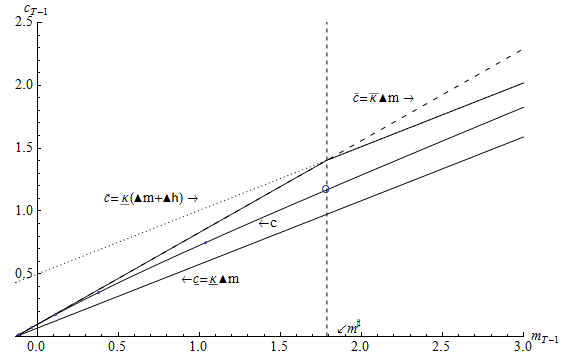
\includegraphics{./Figures/IntExpFOCInvPesReaOptNeed45Plot}
      \caption{45 Degree Line as Another Upper Bound}
      \label{fig:IntExpFOCInvPesReaOptNeed45Plot}
    \end{figure}

    \hypertarget{IntExpFOCInvPesReaOptNeed45ValuePlot}{}
    \begin{figure}
      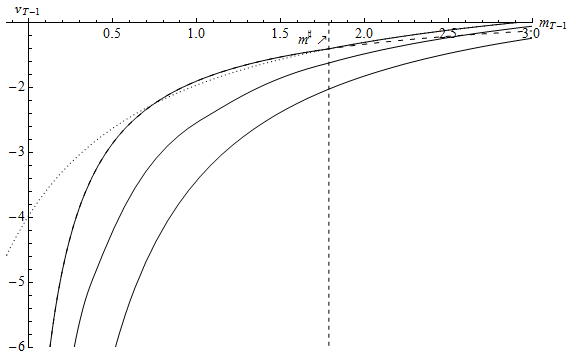
\includegraphics{./Figures/IntExpFOCInvPesReaOptNeed45ValuePlot}
      \caption{A Constrained Optimist's Value Function as Another Upper Bound}
      \label{fig:IntExpFOCInvPesReaOptNeed45ValuePlot}
    \end{figure}

  \end{comment}

  \newcommand{\mtCusp}{\ensuremath{\mNrm_{t}^{\#}}}
  % \newcommand{\aboveMin \mtCusp}{\ensuremath{\aboveMin \mNrm_{t}^{\#}}}
\end{verbatimwrite}
\cite{BufferStockTheory} derives an upper limit  $\MaxMPC_{t}$ for the MPC as $m_{t}$
approaches its lower bound.  Using this
fact plus the strict concavity of the consumption function yields the
proposition that
\begin{eqnarray}
\cFunc_{t}(\ushort{m}_{t}+\aboveMin \mRat_{t}) & < \MaxMPC_{t} \aboveMin \mRat_{t}.
\end{eqnarray}

The solution method described above does not guarantee that
approximated consumption will respect this constraint between gridpoints, and a failure to
respect the constraint can occasionally cause computational problems in solving
or simulating the model.  Here, we
describe a method for constructing an approximation that always
satisfies the constraint.

\begin{comment} % Old text needs to be revised or eliminated
That is, the realist's consumption function is bounded from above by both
the \textit{unconstrained} optimist's problem already treated, as well as
by the \textit{constrained} optimist's problem, which is a 45 degree line
originating from $\ushort{m}_{t}$ on the $m$-axis, as shown in
Figure~\ref{fig:IntExpFOCInvPesReaOptNeed45Plot}. The same is true for
the value function, as illustrated in Figure
\ref{fig:IntExpFOCInvPesReaOptNeed45ValuePlot}.

\hypertarget{IntExpFOCInvPesReaOptNeed45Plot}{}
\begin{figure}
        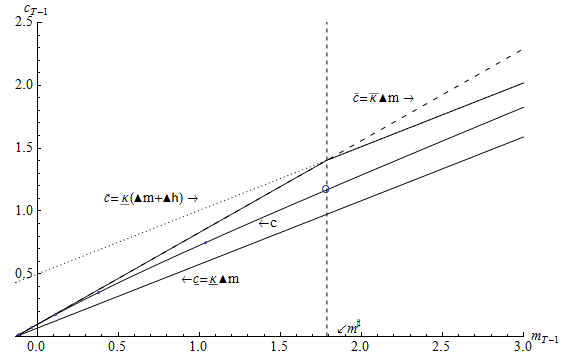
\includegraphics{./Figures/IntExpFOCInvPesReaOptNeed45Plot}
        \caption{45 Degree Line as Another Upper Bound}
        \label{fig:IntExpFOCInvPesReaOptNeed45Plot}
\end{figure}

\hypertarget{IntExpFOCInvPesReaOptNeed45ValuePlot}{}
\begin{figure}
        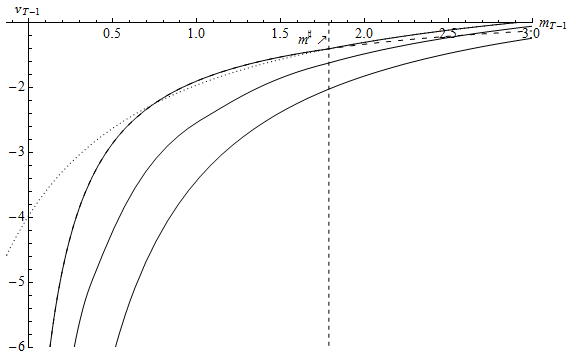
\includegraphics{./Figures/IntExpFOCInvPesReaOptNeed45ValuePlot}
        \caption{A Constrained Optimist's Value Function as Another Upper Bound}
        \label{fig:IntExpFOCInvPesReaOptNeed45ValuePlot}
\end{figure}

\end{comment}

\newcommand{\mtCusp}{\ensuremath{\mRat_{t}^{\#}}}
%\newcommand{\aboveMin \mtCusp}{\ensuremath{\aboveMin \mRat_{t}^{\#}}}
\unskip

\begin{verbatimwrite}{./Equations/mtCusp.tex}
  Defining $\mtCusp$ as the `cusp' point where the two upper bounds
  intersect:
  \begin{equation*}\begin{gathered}\begin{aligned}
        \left(\aboveMin \mtCusp+\aboveMin \hEnd_{t}\right)\MPCmin_{t}  & =  \MPCmax_{t} \aboveMin \mtCusp \\
        \aboveMin \mtCusp  & =  \frac{\MPCmin_{t}\aboveMin \hEnd_{t}}{(1-\MPCmin_{t})\MPCmax_{t}} \\
        \mtCusp  & =  \frac{\MPCmin_{t}\hEnd_{t}-\hEndMin_{t}}{(1-\MPCmin_{t})\MPCmax_{t}},
      \end{aligned}\end{gathered}\end{equation*}
\end{verbatimwrite}
  Defining $\mtCusp$ as the `cusp' point where the two upper bounds
  intersect:
  \begin{equation*}\begin{gathered}\begin{aligned}
    \left(\aboveMin \mtCusp+\aboveMin \hEnd_{t}\right)\MinMPC_{t}  & =  \MaxMPC_{t} \aboveMin \mtCusp \\
    \aboveMin \mtCusp  & =  \frac{\MinMPC_{t}\aboveMin \hEnd_{t}}{(1-\MinMPC_{t})\MaxMPC_{t}} \\
    \mtCusp  & =  \frac{\MinMPC_{t}\hEnd_{t}-\hEndMin_{t}}{(1-\MinMPC_{t})\MaxMPC_{t}},
  \end{aligned}\end{gathered}\end{equation*}
\unskip
\begin{verbatimwrite}{./Equations/TighterUpperBound.tex}
  we want to construct a consumption function for $m_{t} \in (\ushort{m}_{t}, \mtCusp]$ that respects the 
  tighter upper bound:
  \begin{center}
    \begin{tabular}{rcl}
      $ \aboveMin \mNrm_{t} \MPCmin_{t} < $ & $ \cFunc_{t}(\ushort{m}_{t}+\aboveMin \mNrm_{t}) $ & $< \MPCmax_{t} \aboveMin \mNrm_{t} $
      % \\  $-\aboveMin \mNrm_{t} \MPCmin_{t} > $ & $ -\cFunc_{t}(\ushort{m}_{t}+\aboveMin \mNrm_{t}) $ & $> -\aboveMin \mNrm_{t} $
      \\  $ \aboveMin \mNrm_{t}(\MPCmax_{t}- \MPCmin_{t}) > $ & $ \MPCmax_{t} \aboveMin \mNrm_{t}-\cFunc_{t}(\ushort{m}_{t}+\aboveMin \mNrm_{t}) $ & $> 0$
      \\  $1 > $ & $ \left(\frac{\MPCmax_{t} \aboveMin \mNrm_{t}-\cFunc_{t}(\ushort{m}_{t}+\aboveMin \mNrm_{t})}{\aboveMin \mNrm_{t}(\MPCmax_{t}- \MPCmin_{t})}\right) $ & $> 0$.
    \end{tabular}
  \end{center}
\end{verbatimwrite}
  we want to construct a consumption function for $m_{t} \in (\ushort{m}_{t}, \mtCusp]$ that respects the
  tighter upper bound:
  \begin{center}
    \begin{tabular}{rcl}
      $ \aboveMin \mRat_{t} \MinMPC_{t} < $ & $ \cFunc_{t}(\ushort{m}_{t}+\aboveMin \mRat_{t}) $ & $< \MaxMPC_{t} \aboveMin \mRat_{t} $
      % \\  $-\aboveMin \mRat_{t} \MinMPC_{t} > $ & $ -\cFunc_{t}(\ushort{m}_{t}+\aboveMin \mRat_{t}) $ & $> -\aboveMin \mRat_{t} $
      \\  $ \aboveMin \mRat_{t}(\MaxMPC_{t}- \MinMPC_{t}) > $ & $ \MaxMPC_{t} \aboveMin \mRat_{t}-\cFunc_{t}(\ushort{m}_{t}+\aboveMin \mRat_{t}) $ & $> 0$
      \\  $1 > $ & $ \left(\frac{\MaxMPC_{t} \aboveMin \mRat_{t}-\cFunc_{t}(\ushort{m}_{t}+\aboveMin \mRat_{t})}{\aboveMin \mRat_{t}(\MaxMPC_{t}- \MinMPC_{t})}\right) $ & $> 0$.
    \end{tabular}
  \end{center}
\unskip

\begin{verbatimwrite}{./Equations/koppaLo.tex}
  Again defining $\mu_{t} =\log \aboveMin \mNrm_{t}$, the object in the middle of the inequality is
  \begin{equation*}\begin{gathered}\begin{aligned}
        \Lo{\koppa}_{t}(\mu_{t})  & \equiv  \frac{\MPCmax_{t}-\cFunc_{t}(\ushort{m}_{t}+e^{\mu_{t}})e^{-\mu_{t}}}{\MPCmax_{t}-\MPCmin_{t}} \label{eq:koppaL} 
        \MPCMatch{\\ \Lo{\koppa}^{\mu}_{t}(\mu_{t})  & = \frac{\cFunc_{t}(\ushort{m}_{t}+e^{\mu_{t}})e^{-\mu_{t}}-\MPCFunc_{t}^{m}(\ushort{m}_{t}+e^{\mu_{t}})}{\MPCmax_{t}-\MPCmin_{t}}}{} .
      \end{aligned}\end{gathered}\end{equation*}
\end{verbatimwrite}
  Again defining $\mu_{t} =\log \aboveMin \mRat_{t}$, the object in the middle of the inequality is
  \begin{equation*}\begin{gathered}\begin{aligned}
    \Lo{\koppa}_{t}(\mu_{t})  & \equiv  \frac{\MaxMPC_{t}-\cFunc_{t}(\ushort{m}_{t}+e^{\mu_{t}})e^{-\mu_{t}}}{\MaxMPC_{t}-\MinMPC_{t}} \label{eq:koppaL}
                                        \MPCMatch{\\ \Lo{\koppa}^{\mu}_{t}(\mu_{t})  & = \frac{\cFunc_{t}(\ushort{m}_{t}+e^{\mu_{t}})e^{-\mu_{t}}-\MPCFunc_{t}^{m}(\ushort{m}_{t}+e^{\mu_{t}})}{\MaxMPC_{t}-\MinMPC_{t}}}{} .
  \end{aligned}\end{gathered}\end{equation*}
\unskip

\begin{verbatimwrite}{./cctwMoM/TighterThreeFuncs.tex}
  As $m_{t}$ approaches
  $-\ushort{m}_{t}$, $\Lo{\koppa}_{t}(\mu_{t})$ converges to zero, while as $m_{t}$
  approaches $+\infty$, $\Lo{\koppa}_{t}(\mu_{t})$ approaches $1$.  

  As before, we can derive an approximated consumption function; call it
  $\Alt{\Lo{\cFunc}}_{t}$.  This function will clearly do a better job approximating the consumption
  function for low values of $\mNrm_{t}$ while the previous approximation will perform better
  for high values of $\mNrm_{t}$.  

  For middling values of $\mNrm$ it is not clear which of these
  functions will perform better.  However, an alternative is available
  which performs well.  Define the highest gridpoint below $\mtCusp$ as
  $\bar{\check{\mNrm}}_{t}^{\#}$ and the lowest gridpoint above $\mtCusp$ as
  $\ushort{\hat{\mNrm}}_{t}^{\#}$.  Then there will be a unique interpolating
  polynomial that matches the level and slope of the consumption function
  at these two points.  Call this function $\tilde{\cFunc}_{t}(\mNrm)$.  

  Using indicator functions that are zero everywhere except for specified intervals,
\end{verbatimwrite}
  As $m_{t}$ approaches
  $-\ushort{m}_{t}$, $\Lo{\koppa}_{t}(\mu_{t})$ converges to zero, while as $m_{t}$
  approaches $+\infty$, $\Lo{\koppa}_{t}(\mu_{t})$ approaches $1$.

  As before (in equation \eqref{eq:vEndtdefn}), we can derive an approximated consumption function; call it
  $\Alt{\Lo{\cFunc}}_{t}$.  This function will clearly do a better job approximating the consumption
  function for low values of $\mRat_{t}$ while the previous approximation will perform better
  for high values of $\mRat_{t}$.

  For middling values of $\mRat$ it is not clear which of these
  functions will perform better.  However, an alternative is available
  which performs well.  Define the highest gridpoint below $\mtCusp$ as
  $\bar{\check{\mRat}}_{t}^{\#}$ and the lowest gridpoint above $\mtCusp$ as
  $\ushort{\hat{\mRat}}_{t}^{\#}$.  Then there will be a unique interpolating
  polynomial that matches the level and slope of the consumption function
  at these two points.  Call this function $\tilde{\cFunc}_{t}(\mRat)$.

  Using indicator functions that are zero everywhere except for specified intervals,
\unskip
\begin{verbatimwrite}{./Equations/TighterThreeEqns.tex}
  \begin{equation*}\begin{gathered}\begin{aligned}
        \pmb{1}_{\text{Lo}}(\mNrm)  & = 1 \text{~if $          \mNrm \leq  \bar{\check{\mNrm}}_{t}^{\#} \phantom{< \mNrm <   \ushort{\hat{\mNrm}}_{t}^{\#}          \leq \mNrm}$}
        \\  \pmb{1}_{\text{Mid}}(\mNrm)  & = 1 \text{~if $\phantom{ \mNrm \leq}~ \bar{\check{\mNrm}}_{t}^{\#}          < \mNrm <   \ushort{\hat{\mNrm}}_{t}^{\#} \phantom{\leq \mNrm}$}
        \\  \pmb{1}_{\text{Hi}}(\mNrm)  & = 1 \text{~if $\phantom{ \mNrm \leq  ~\bar{\check{\mNrm}}_{t}^{\#}          < \mNrm < } \ushort{\hat{\mNrm}}_{t}^{\#}           \leq \mNrm$}
      \end{aligned}\end{gathered}\end{equation*}
  we can define a well-behaved approximating consumption function
  \begin{equation}\begin{gathered}\begin{aligned}
        \Alt{\cFunc}_{t}  & = \pmb{1}_{\text{Lo}} \Alt{\Lo{\cFunc}}_{t} + \pmb{1}_{\text{Mid}} \Alt{\tilde{\cFunc}}_{t}+\pmb{1}_{\text{Hi}} \Alt{\Hi{\cFunc}}_{t}.
      \end{aligned}\end{gathered}\end{equation} 
\end{verbatimwrite}
  \begin{equation*}\begin{gathered}\begin{aligned}
        \pmb{1}_{\text{Lo}}(\mNrm)  & = 1 \text{~if $          \mNrm \leq  \bar{\check{\mNrm}}_{t}^{\#} \phantom{< \mNrm <   \ushort{\hat{\mNrm}}_{t}^{\#}          \leq \mNrm}$}
        \\  \pmb{1}_{\text{Mid}}(\mNrm)  & = 1 \text{~if $\phantom{ \mNrm \leq}~ \bar{\check{\mNrm}}_{t}^{\#}          < \mNrm <   \ushort{\hat{\mNrm}}_{t}^{\#} \phantom{\leq \mNrm}$}
        \\  \pmb{1}_{\text{Hi}}(\mNrm)  & = 1 \text{~if $\phantom{ \mNrm \leq  ~\bar{\check{\mNrm}}_{t}^{\#}          < \mNrm < } \ushort{\hat{\mNrm}}_{t}^{\#}           \leq \mNrm$}
      \end{aligned}\end{gathered}\end{equation*}
  we can define a well-behaved approximating consumption function
  \begin{equation}\begin{gathered}\begin{aligned}
        \Alt{\cFunc}_{t}  & = \pmb{1}_{\text{Lo}} \Alt{\Lo{\cFunc}}_{t} + \pmb{1}_{\text{Mid}} \Alt{\tilde{\cFunc}}_{t}+\pmb{1}_{\text{Hi}} \Alt{\Hi{\cFunc}}_{t}.
      \end{aligned}\end{gathered}\end{equation}
\unskip

\begin{verbatimwrite}{./cctwMoM/TighterThreeFuncsExplain.tex}
  This just says that, for each interval, we use the approximation that
  is most appropriate.  The function is continuous and
  once-differentiable everywhere, and is therefore well behaved for
  computational purposes.
  \begin{comment}
    In practice, in our problem the difference due to this refinement is displayed in Figure \ref{fig:IntExpFOCInvPesReaOpt45GapPlot}.
    \hypertarget{IntExpFOCInvPesReaOpt45GapPlot}{}
    \begin{figure}
      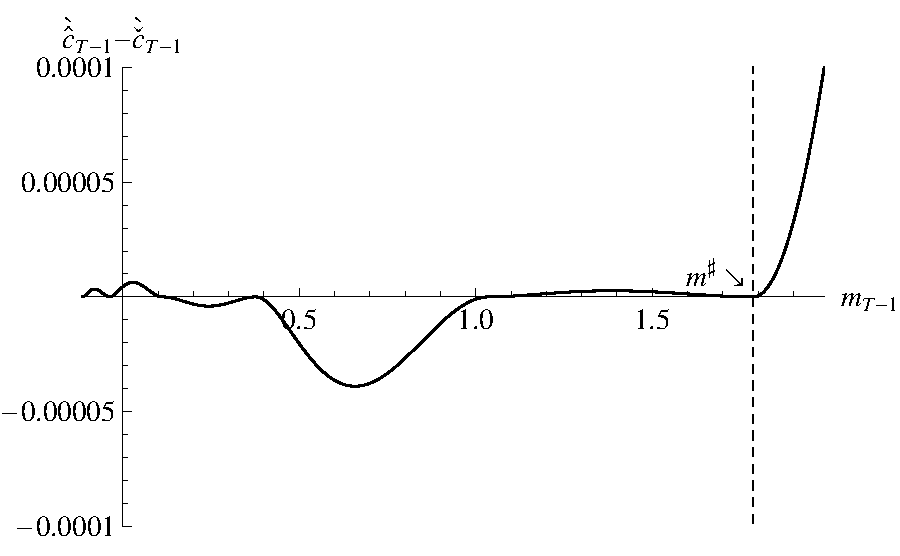
\includegraphics{./Figures/IntExpFOCInvPesReaOpt45GapPlot}
      \caption{Difference Between $\Alt{\Hi{\cFunc}}_{L, T-1}$ and $\Alt{\Hi{\cFunc}}_{H,T-1}$ is Small}
      \label{fig:IntExpFOCInvPesReaOpt45GapPlot}
    \end{figure}
  \end{comment}

  We now construct an upper-bound value function implied for a consumer whose spending behavior
  is consistent with the refined upper-bound consumption rule.  

  For $\mNrm_{t} \geq \mNrm_{t}^{\#}$, this consumption rule is the same as before,
  so the constructed upper-bound value function is also the same.  However, for 
  values $\mNrm_{t} < \mNrm_{t}^{\#}$ matters are slightly more complicated.  

  Start with the fact that at the cusp point, 
  \begin{equation*}\begin{gathered}\begin{aligned}
        \bar{\vFunc}_{t}(\mtCusp)  & = \uFunc(\bar{\cNrm}_{t}(\mtCusp))\mathbb{C}_{t}^{T} \\
        & =  \uFunc(\aboveMin \mtCusp  \MPCmax_{t})\mathbb{C}_{t}^{T}
        .
      \end{aligned}\end{gathered}\end{equation*}

  But for \textit{all} $\mNrm_{t}$,
  \begin{equation*}\begin{gathered}\begin{aligned}
        \bar{\vFunc}_{t}(\mNrm)  & = \uFunc(\bar{\cNrm}_{t}(\mNrm))+ \bar{\vEndStget}(\mNrm-\bar{\cNrm}_{t}(\mNrm)),
      \end{aligned}\end{gathered}\end{equation*}
  and we assume that for the consumer below the cusp point consumption is given by $\MPCmax \aboveMin \mNrm_{t}$ so for $\mNrm_{t}< \mtCusp$
  \begin{equation*}\begin{gathered}\begin{aligned}
        \bar{\vFunc}_{t}(\mNrm)  & = \uFunc( \MPCmax_{t} \aboveMin \mNrm)+ \bar{\vEndStget}((1-\MPCmax_{t})\aboveMin \mNrm),
      \end{aligned}\end{gathered}\end{equation*}
  which is easy to compute because $\bar{\vEndStget}(\aNrm_{t}) = \DiscFac \bar{\vFunc}_{t+1}(\aNrm_{t}\RNrm+1)$
  where $\bar{\vFunc}_{t}$ is as defined above because a consumer who ends the current period with assets exceeding
  the lower bound will not expect to be constrained next period.  (Recall again that we are merely constructing an object that is guaranteed to be an \textit{upper bound} for the value that the `realist' consumer will experience.)  At the gridpoints defined by the solution of the 
  consumption problem can then construct
  \begin{equation*}\begin{gathered}\begin{aligned}
        \bar{\vInv}_{t}(\mNrm)  & = ((1-\CRRA)\bar{\vFunc}_{t}(\mNrm))^{1/(1-\CRRA)}
      \end{aligned}\end{gathered}\end{equation*}
  \MPCMatch{and its derivatives}{} which yields the appropriate vector for constructing $\check{\Chi}$ and $\check{\Koppa}$.  The rest of the procedure is analogous to that performed for the consumption rule and is thus omitted for brevity.

\end{verbatimwrite}

This just says that, for each interval, we use the approximation that
is most appropriate.  The function is continuous and
once-differentiable everywhere, and is therefore well behaved for
computational purposes.

\begin{comment}
In practice, in our problem the difference due to this refinement is displayed in Figure \ref{fig:IntExpFOCInvPesReaOpt45GapPlot}.
\hypertarget{IntExpFOCInvPesReaOpt45GapPlot}{}
\begin{figure}
        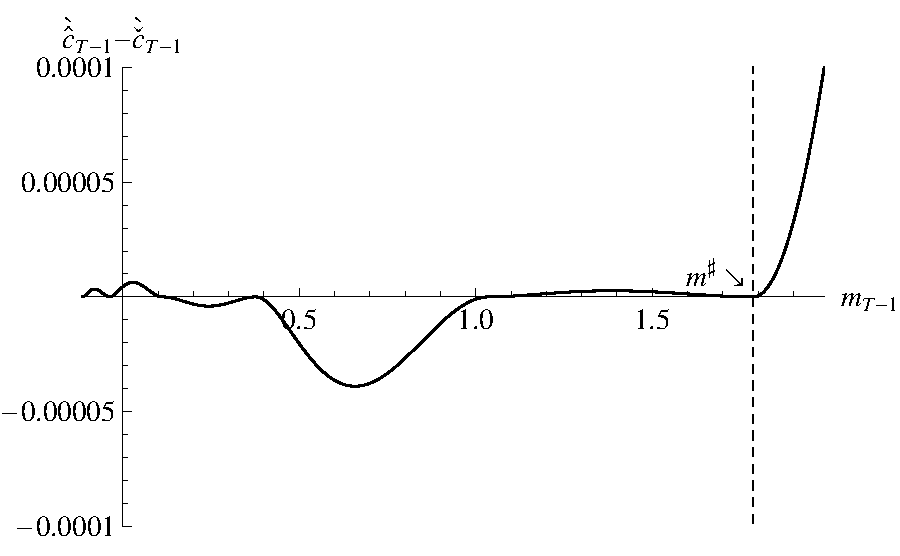
\includegraphics{./Figures/IntExpFOCInvPesReaOpt45GapPlot}
        \caption{Difference Between $\Alt{\Hi{\cFunc}}_{L, T-1}$ and $\Alt{\Hi{\cFunc}}_{H,T-1}$ is Small}
        \label{fig:IntExpFOCInvPesReaOpt45GapPlot}
\end{figure}
\end{comment}

We now construct an upper-bound value function implied for a consumer whose spending behavior
is consistent with the refined upper-bound consumption rule.

For $\mRat_{t} \geq \mRat_{t}^{\#}$, this consumption rule is the same as before,
so the constructed upper-bound value function is also the same.  However, for
values $\mRat_{t} < \mRat_{t}^{\#}$ matters are slightly more complicated.

Start with the fact that at the cusp point,
\begin{eqnarray*}
  \bar{\vFunc}_{t}(\mtCusp) & = & \util(\bar{\cRat}_{t}(\mtCusp))\mathbb{C}_{t}^{T} \\
  &=& \util(\aboveMin \mtCusp  \MaxMPC_{t})\mathbb{C}_{t}^{T}
.
\end{eqnarray*}

But for \textit{all} $\mRat_{t}$,
\begin{eqnarray*}
  \bar{\vFunc}_{t}(\mRat) & = & \util(\bar{\cRat}_{t}(\mRat))+ \bar{\vEnd}_{t}(\mRat-\bar{\cRat}_{t}(\mRat)),
\end{eqnarray*}
and we assume that for the consumer below the cusp point consumption is given by $\MaxMPC \aboveMin \mRat_{t}$ so for $\mRat_{t}< \mtCusp$
\begin{eqnarray*}
  \bar{\vFunc}_{t}(\mRat) & = & \util( \MaxMPC_{t} \aboveMin \mRat)+ \bar{\vEnd}_{t}((1-\MaxMPC_{t})\aboveMin \mRat),
\end{eqnarray*}
which is easy to compute because $\bar{\vEnd}_{t}(\aRat_{t}) = \Discount \bar{\vFunc}_{t+1}(\aRat_{t}\Rnorm+1)$
where $\bar{\vFunc}_{t}$ is as defined above because a consumer who ends the current period with assets exceeding
the lower bound will not expect to be constrained next period.  (Recall again that we are merely constructing an object that is guaranteed to be an \textit{upper bound} for the value that the `realist' consumer will experience.)  At the gridpoints defined by the solution of the
consumption problem can then construct
\begin{eqnarray*}
  \bar{\vInv}_{t}(\mRat) & = & ((1-\CRRA)\bar{\vFunc}_{t}(\mRat))^{1/(1-\CRRA)}
\end{eqnarray*}
\MPCMatch{and its derivatives}{} which yields the appropriate vector for constructing $\check{\Chi}$ and $\check{\Koppa}$.  The rest of the procedure is analogous to that performed for the consumption rule and is thus omitted for brevity.

\unskip

\hypertarget{Extension-A-Stochastic-Interest-Factor}{}
\subsection{Extension: A Stochastic Interest Factor}


Thus far we have assumed that the interest factor is constant at $\Rfree$.  Extending the
previous derivations to allow for a perfectly forecastable time-varying interest factor $\Rfree_{t}$ 
would be trivial.  Allowing for a stochastic interest factor is less trivial.  


The easiest case is where the interest factor is i.i.d.,
\begin{verbatimwrite}{./Equations/distRisky.tex}
  \begin{equation}\begin{gathered}\begin{aligned}
        \log \Risky_{t+n} & \sim & \mathcal{N}(\rfree + \eprem - \sigma^{2}_{\risky}/2,\sigma^{2}_{\risky}) ~\forall~n>0 \label{eq:distRisky}
      \end{aligned}\end{gathered}\end{equation}
\end{verbatimwrite}
  \begin{eqnarray}
    \log \Risky_{t+n} & \sim & \mathcal{N}(\rfree + \eprem - \sigma^{2}_{\risky}/2,\sigma^{2}_{\risky}) ~\forall~n>0 \label{eq:distRisky}
  \end{eqnarray}
\unskip
where $\eprem$ is the risk premium and the $\sigma^{2}_{\risky}/2$ adjustment to the mean log return
guarantees that an increase in $\sigma^{2}_{\risky}$ constitutes a mean-preserving spread in the level of the return.  

This case is reasonably straightforward because \cite{merton:restat} and \cite{samuelson:portfolio} showed
that for a consumer without labor income (or with perfectly forecastable labor income) the consumption
function is linear, with an infinite-horizon MPC\footnote{See \handoutC{CRRA-RateRisk} for a derivation.}
\begin{equation}\begin{gathered}\begin{aligned}
      \MPC  & = 1- \left(\DiscFac  \Ex_{t}[\Risky_{t+1}^{1-\CRRA}]\right)^{1/\CRRA} \label{eq:MPCExact}
    \end{aligned}\end{gathered}\end{equation}
and in this case the previous analysis applies once we substitute this MPC for the one that characterizes 
the perfect foresight problem without rate-of-return risk.  

The more realistic case where the interest factor has some serial correlation is more complex.  We consider 
the simplest case that captures the main features of empirical interest rate dynamics: An AR(1) process.  Thus
the specification is 
\begin{equation}\begin{gathered}\begin{aligned}
      \risky_{t+1}-\risky  & = (\risky_{t}-\risky) \gamma + \epsilon_{t+1} 
    \end{aligned}\end{gathered}\end{equation}
where $\risky$ is the long-run mean log interest factor, $0 < \gamma < 1$ is the AR(1) serial correlation
coefficient, and $\epsilon_{t+1}$ is the stochastic shock.  

The consumer's problem in this case now has two state variables, $\mNrm_{t}$ and $\risky_{t}$, and 
is described by
\begin{equation}\begin{gathered}\begin{aligned}
      \null{\vFunc}_{t}({m}_{t},\risky_{t})  & = \max_{{c}_{t}} ~ \uFunc({c}_{t})+
      \Ex_{t}[{\DiscFac}_{t+1}\PermGroFac_{t+1}^{1-\CRRA}\null{\vFunc}_{t+1}({m}_{t+1},\risky_{t+1})] \label{vtNormRisky}
      \\         & \text{s.t.} &   \nonumber \\
      {a}_{t}    & = {m}_{t}-{c}_{t} \nonumber
      \\      \risky_{t+1}-\risky  & = (\risky_{t}-\risky)\gamma + \epsilon_{t+1} \notag
      \\      \Risky_{t+1}  & = \exp(\risky_{t+1}) \notag
      \\      {m}_{t+1}  & = \underbrace{\left(\Risky_{t+1}/\PermGroFac_{t+1}\right)}_{\equiv \Rprod_{t+1}}{a}_{t}+\TranShkEmp_{t+1} \nonumber.
    \end{aligned}\end{gathered}\end{equation}

% Kiichi: I will need you to read the literature and figure out how exactly we want to choose the Markov points and transition probabilities.
% When done, you will fill in the [how] text below.

We approximate the AR(1) process by a Markov transition matrix using standard techniques.  The stochastic interest factor is allowed to take 
on 11 values centered around the steady-state value $\risky$.  Given this Markov transition matrix,
\textit{conditional} on the Markov AR(1) state the consumption functions for the `optimist' and the `pessimist' will still be linear, 
with identical MPC's that are computed numerically.  Given these MPC's, the (conditional) realist's consumption function can be computed for each Markov state, and the converged consumption rules constitute the solution contingent on the dynamics of the stochastic
interest rate process.  

In principle, this refinement should be combined with the previous one;
further exposition of this combination is omitted here because no new
insights spring from the combination of the two techniques.



\hypertarget{Imposing-Artificial-Borrowing-Constraints}{}
\subsection{Imposing `Artificial' Borrowing Constraints}

Optimization problems often come with additional constraints that must
be satisfied.  Particularly common is an `artificial' liquidity constraint that
prevents the consumer's net worth from falling below some value, often
zero.\footnote{The word artificial is chosen only because of its clarity in distinguishing
  this from the case of the `natural' borrowing constraint examined above; no derogation is
  intended -- constraints of this kind certainly exist in the real world.}  The problem then becomes
\begin{equation*}\begin{gathered}\begin{aligned}
      {\vFunc}_{T-1}({m}_{T-1})  & = \max_{\cNrm_{T-1}} ~~ \uFunc({c}_{T-1}) + \Ex_{T-1} [\DiscFac \PermGroFac_{T}^{1-\CRRA}{\vFunc}_{T}({m}_{T})] \label{eq:ConstrArt}
      \\ & \mbox{s.t.}&  \nonumber
      \\ {a}_{T-1}  & = {m}_{T-1} - {c}_{T-1}
      \\ {m}_{T}  & = \RNrm_{T} {a}_{T-1} + \TranShkEmp_{T}
      \\ {a}_{T-1} & \geq 0 .
    \end{aligned}\end{gathered}\end{equation*}

\ifthenelse{\boolean{MyNotes}}{\marginpar{\tiny Constraint binds whenever you would like to consume more than current resources.}}{}

By definition, the constraint will bind if the unconstrained consumer
would choose a level of spending that would violate the constraint.
Here, that means that the constraint binds if the ${c}_{T-1}$
that satisfies the unconstrained FOC
\begin{equation}\begin{gathered}\begin{aligned}
      {c}_{T-1}^{-\CRRA}  & = \vFunc^{{a}}_{T^{+}-1}({m}_{T-1}-{c}_{T-1}) \label{eq:cUnc}
    \end{aligned}\end{gathered}\end{equation}
is greater than ${m}_{T-1}$.  Call $\grave{\cFunc}^{\ast}_{T-1}$ the approximated function
returning the level of ${c}_{T-1}$ that satisfies \eqref{eq:cUnc}.
Then the approximated constrained optimal consumption function will be
\begin{verbatimwrite}{./Equations/LiqCons.tex}
  \begin{equation}\begin{gathered}\begin{aligned}
        \grave{\cFunc}_{T-1}({m}_{T-1})  & = \min[{m}_{T-1},\grave{\cFunc}^{\ast}_{T-1}({m}_{T-1})] \label{eq:LiqCons}.
      \end{aligned}\end{gathered}\end{equation}
\end{verbatimwrite}
\begin{eqnarray}
        \grave{\cFunc}_{T-1}({m}_{T-1}) & = & \min[{m}_{T-1},\grave{\cFunc}^{\ast}_{T-1}({m}_{T-1})] \label{eq:LiqCons}.
\end{eqnarray}
\unskip

\ifthenelse{\boolean{MyNotes}}{\marginpar{\tiny Read this carefully
    before class.  Intuition: consider discounted mv of saving zero.  If
    consume everything and get the same $\uFunc^{{c}}$, then happy.  If
    consumed $\TranShkEmp$ less, mv of saving would be $> \uFunc^{{c}}(c).$}}{}

The introduction of the constraint also introduces a sharp
nonlinearity in all of the functions at the point where the constraint
begins to bind.  As a result, to get solutions that are anywhere close
to numerically accurate it is useful to augment the grid of values of
the state variable to include the exact value at which the constraint
ceases to bind.  Fortunately, this is easy to calculate.  We know that
when the constraint is binding the consumer is saving nothing, which
yields marginal value of $\vFunc^{{a}}_{T^{+}-1}(0)$. Further, when the
constraint is binding, ${c}_{T-1} = {m}_{T-1}$.  Thus, the largest
value of consumption for which the constraint is binding will be the
point for which the marginal utility of consumption is exactly equal
to the (expected, discounted) marginal value of saving 0.  We know
this because the marginal utility of consumption is a downward-sloping
function and so if the consumer were to consume $\tinyAmount$ more,
the marginal utility of that extra consumption would be \textit{below}
the (discounted, expected) marginal utility of saving, and thus the
consumer would engage in positive saving and the constraint would no
longer be binding.  Thus the level of ${m}_{T-1}$ at which the
constraint stops binding is:\footnote{The logic here repeats an insight from \cite{deatonLiqConstr}.}
\begin{equation}\begin{gathered}\begin{aligned}
      \uFunc^{{c}}({m}_{T-1})  & = \vFunc^{{a}}_{T^{+}-1}(0)  \nonumber \\
      {m}_{T-1}  & = (\vFunc^{{a}}_{T^{+}-1}(0))^{(-1/\CRRA)}  \nonumber
      \\        & = \cFunc_{T^{+}-1}(0). \label{eq:LCbindsTm1}
    \end{aligned}\end{gathered}\end{equation}

\hypertarget{cVScCon}{}
\begin{figure}
  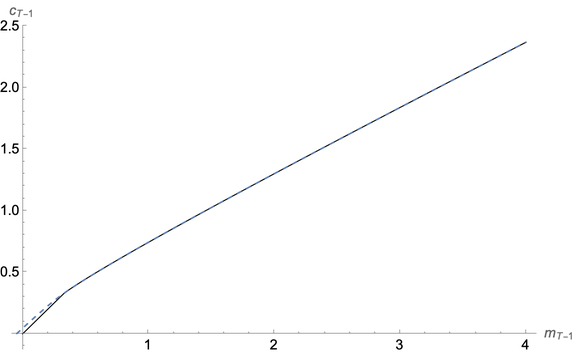
\includegraphics{./Figures/cVScCon}
  \caption{Constrained (solid) and Unconstrained (dashed) Consumption}
  \label{fig:cVScCon}
\end{figure}

The constrained problem is solved by
\texttt{2periodIntExpFOCInvPesReaOptCon.m}; the resulting consumption
rule is shown in Figure \ref{fig:cVScCon}. For comparison purposes,
the approximate consumption rule from Figure \ref{fig:cVScCon} is
reproduced here as the solid line. The presence of the liquidity
constraint requires three changes to the procedures outlined above:
\begin{enumerate}
\item We redefine
  $\hEndMin_{t}$, which now is the PDV of receiving
  $\TranShkEmp_{t+1}=\TranShkEmpMin$ next period and
  $\TranShkEmp_{t+n}=0~\forall~n>1$ -- that is, the pessimist believes he
  will receive nothing beyond period $t+1$
\item We augment the end-of-period \texttt{aVec} with zero and with a point with a small positive value so that the generated 
  \texttt{mVec} will the binding point $\mNrm^{\#}$ and a point just above it (so that we can better capture the curvature
  around that point)
\item We redefine the optimal consumption rule as
  in equation (\ref{eq:LiqCons}).  This ensures that the
  liquidity-constrained `realist' will consume more than the redefined
  `pessimist,' so that we will have $\koppa$ still between $0$ and $1$
  and the `method of moderation' will proceed smoothly. 
\end{enumerate}

As expected, the
liquidity constraint only causes a divergence between the two
functions at the point where the optimal unconstrained consumption
rule runs into the 45 degree line.

\hypertarget{Recursions}{}
\section{Recursion}\label{sec:recursion}
\hypertarget{Theory}{}
\subsection{Theory}
Before we solve for periods earlier than $T-1$, we assume for
convenience that in each such period a liquidity constraint exists of
the kind discussed above, preventing ${c}$ from exceeding ${m}$. This
simplifies things a bit because now we can always consider an
\texttt{aVec} that starts with zero as its smallest element.

Recall now equations~(\ref{eq:vEndPrimetOfc}) and (\ref{eq:upEqbetaOp}):
\begin{equation*}\begin{gathered}\begin{aligned}
      \vPEndStget({a}_{t})  & = \Ex_{t}[\DiscFac \Rfree \PermGroFac_{t+1}^{-\CRRA}
      \uFunc^{{c}}(\cFunc_{t+1}(\RNrm_{t+1} {a}_{t}+{\TranShkEmp}_{t+1}))]
      \\\uFunc^{{c}}({c}_{t})   & = \vEndStget^{\prime}({m}_{t}-{c}_{t}).
    \end{aligned}\end{gathered}\end{equation*}
Assuming that the problem has been solved up to period $t+1$ (and thus
assuming that we have an approximated $\Alt{\cFunc}_{t+1}({m}_{t+1})$), our solution method essentially
involves using these two equations in succession to work back
progressively from period $T-1$ to the beginning of life.  Stated
generally, the method is as follows.  (Here, we use the original, rather than the ``refined,'' method for 
constructing consumption functions; the generalization of the algorithm below to use the refined method presents
no difficulties.)

\begin{enumerate}
  \ifthenelse{\boolean{MyNotes}}{\marginpar{\tiny Point out that we
      are defining $\vEndStget^{\prime}$ here by the literal summation
      operation \eqref{eq:vEndeq}.}}{}

\item For the grid of values ${a}_{t,i}$ in \texttt{aVec}$_{t}$, numerically calculate the values
  of $\cFunc_{\overline{t}}({a}_{t,i})$ and $\cFunc_{\overline{t}}^{{a}}({a}_{t,i})$,
  \begin{verbatimwrite}{./Equations/vEndeq.tex}
    \begin{equation}\begin{gathered}\begin{aligned}
          \cFunc_{\overline{t},i}  & = \left(\vEndStget^{\prime}({a}_{t,i})\right)^{-1/\CRRA},
          \\                             & = \left(\DiscFac \Ex_{t} \left[\Rfree \PermGroFac_{t+1}^{-\CRRA}(\grave{\cFunc}_{t+1}(\RNrm_{t+1} {a}_{t,i} +      {\TranShkEmp}_{t+1}))^{-\CRRA}\right]\right)^{-1/\CRRA}, \label{eq:vEndeq}
          \MPCMatch{\\        \cFunc^{a}_{\overline{t},i}  & = -(1/\CRRA)\left(\vEndStget^{\prime}({a}_{t,i})\right)^{-1-1/\CRRA} \vEndStget^{\prime\prime}(\aNrm_{t,i}),}{}
        \end{aligned}\end{gathered}\end{equation}
  \end{verbatimwrite}
  \begin{eqnarray}
        \cEndFunc_{t,i} & = & \left(\vEnd_{t}^{\prime}({a}_{t,i})\right)^{-1/\CRRA},
\\                            & = & \left(\Discount \Ex_{t} \left[\Rfree \PGro_{t+1}^{-\CRRA}(\grave{\cFunc}_{t+1}(\Rnorm_{t+1} {a}_{t,i} +      {\tShkEmp}_{t+1}))^{-\CRRA}\right]\right)^{-1/\CRRA}, \label{eq:vEndeq}
\MPCMatch{\\        \cEndFunc^{a}_{t,i} & = & -(1/\CRRA)\left(\vEnd_{t}^{\prime}({a}_{t,i})\right)^{-1-1/\CRRA} \vEnd_{t}^{\prime\prime}(\aRat_{t,i}),}{}
\end{eqnarray}

  generating vectors of values $\vec{\cFunc}_{t}$\MPCMatch{ and $\vec{\cFunc}^{a}_{\overline{t}}$.}{.}

\item Construct a corresponding vector of values of $\vec{m}_{t}=\vec{\cNrm}_{t}+\vec{\aNrm}_{t}$\MPCMatch{; similarly construct a corresponding list of MPC's $\vec{\MPC}_{t}$ using equation \eqref{eq:MPCfromMPTHC}.}{.}

\item Construct a corresponding vector $\vec{\mu_{t}}$, the levels\MPCMatch{ and first derivatives}{} of $\vec{\koppa}_{t}$, and the levels\MPCMatch{ and first derivatives}{} of $\vec{\chi}_{t}$.

\item Construct an interpolating approximation $\Alt{\chi}_{t}$ that\MPCMatch{ smoothly matches both the level and the slope}{the level} at those points.

\item If we are to approximate the value function, construct a corresponding list of values of $\vec{\vFunc}_{t}$, the levels\MPCMatch{ and first derivatives of $\vec{\Koppa}_{t}$,}{,} and the levels\MPCMatch{ and first derivatives}{} of $\hat{\vec{\Chi}}_{t}$; and construct an interpolating approximation function $\hat{\Chi}_{t}$ that matches those points.
\end{enumerate}

With $\Alt{\chi}_{t}$ in hand, our approximate consumption function
is computed directly from the appropriate substitutions in \eqref{eq:cFuncHi}
and related equations.  With this consumption
rule in hand, we can continue the backwards recursion to period $t-1$
and so on back to the beginning of life.

Note that this loop does not contain steps for constructing
$\hat{\vFunc}_{t}^{\prime}({m}_{t})$. This is because with
$\Alt{\Hi{\cFunc}}_{t}({m}_{t})$ in
hand, we simply \textit{define} $\hat{\vFunc}^{{m}}_{t}({m}_{t}) = \uFunc^{{c}}(\Alt{\Hi{\cFunc}}_{t}({m}_{t}))$
so there is no need to construct interpolating approximations 
- the function arises `free' (or nearly so) from our constructed
$\Alt{\Hi{\cFunc}}_{t}({m}_{t})$ via the usual envelope result (cf.\ \eqref{eq:envelope}).

The program \texttt{multiperiodCon.m}\footnote{There is also a parallel \texttt{multiperiod.m} file that solves the unconstrained multi-period problem.} presents a fairly general and
flexible approach to solving problems of this kind. The essential
structure of the program is a loop that simply works its way back
from an assumed last period of life, using the command
\texttt{AppendTo} to record the interpolated $\grave{\chi}_{t}$ functions
in the earlier time periods back from the end. For a
realistic life cycle problem, it would also be necessary at a
minimum to calibrate a nonconstant path of expected income growth over the
lifetime that matches the empirical profile; allowing for such
a calibration is the reason we have included the $\{\PermGroFac\}_{t}^{T}$
vector in our computational specification of the problem.

\hypertarget{Mathmatica-Background}{}
\subsection{{\Mma}~Background}
{\Mma}~has several features that are useful in solving the
multiperiod problem.

\begin{itemize}
\item It can treat a user-created function as an object just like a
  number or a character.

\item {\Mma}~uses the `list' as its basic data structure.  A
  {\Mma}~`list' is a very powerful and flexible data construct.  A
  list of length N in {\Mma}~can hold essentially anything in each
  of its $Num$ positions - a function, a number, another list, a symbolic
  expression, or any other object that {\Mma}~can recognize.  The
  items at position $i$ in a list named \texttt{ExampleList} are retrieved or
  addressed using the syntax \texttt{ExampleList[[i]]}.

\item The function \texttt{Apply[FuncName\_, DataListName\_]} takes
  the function whose name is \texttt{FuncName} (for example,
  \texttt{Vt}) and the data in \texttt{DataListName} (for example,
  $\{1,19\}$) and returns the result that would have been returned by
  calling the function \texttt{Vt[1,19]}.

\item The function \texttt{Map[FuncToApply\_,DataToApplyItTo\_]} takes
  a list of possible arguments to the function \texttt{FuncToApply} and applies
  that function to each of the elements of that list sequentially.  For
  example, \texttt{Map[Sin,\{1,2,3\}]} would return a list
  \texttt{\{Sin[1],Sin[2],Sin[3]\}}.

\end{itemize}

\hypertarget{Program-Structure}{}
\subsection{Program Structure}

After the usual initializations, the heart of the program works like
this.

\hypertarget{Iteration}{}
\subsubsection{Iteration}

After setting up a variable \texttt{PeriodsToSolve} which defines the
total number of periods that the program will solve, the program sets
up a ``\texttt{Do[SolveAnotherPeriod,\{PeriodsToSolve\}]}'' loop that
runs the function \texttt{SolveAnotherPeriod} the number of times
corresponding to \texttt{PeriodsToSolve}. Every time
\texttt{SolveAnotherPeriod} is run, the interpolated consumption
function for one period of life earlier is calculated. The structure
of the \texttt{SolveAnotherPeriod} function is as follows:
\ifthenelse{\boolean{MyNotes}}{\marginpar{\tiny It's easier to just
    examine the program and discuss it than to try and read this flow
    description.}}{}

\begin{enumerate}

\item Add various period-t parameters to their respective lifecycle lists, which is accomplished by calling the \texttt{AddNewPeriodToParamLifeDates} function.

\item For each ${a}_{t,i}$ in \texttt{aVec}, construct a set of points on the `consumed' function $\cFunc_{\overline{t}}({a})$ as follows:
  \begin{equation}\begin{gathered}\begin{aligned}
        \cFunc_{\overline{t}}({a}_{t,i})  & = \left( \DiscFac \Ex_{t} \left[\Rfree \PermGroFac_{t+1}^{-\CRRA} (\Alt{\Hi{\cFunc}}_{t+1}(\RNrm_{t+1} {a}_{t,i} +         {\TranShkEmp}_{t+1}))^{-\CRRA}\right]\right)^{-1/\CRRA}
        \\                           & = \left(\DiscFac \frac{1}{n_{\TranShkEmp}} \sum_{i=1}^{n_{\TranShkEmp}}\Rfree\left(\PermGroFac_{t+1}^{-\CRRA}(\Alt{\Hi{\cFunc}}_{t+1}(\RNrm_{t+1} {a}_{t,i} +       \TranShkEmp_{i}))^{-\CRRA}\right)\right)^{-1/\CRRA}
      \end{aligned}\end{gathered}\end{equation}
  \MPCMatch{and similarly construct the corresponding derivative with respect to $\aNrm$, $\cFunc_{\overline{t}}^{a}({a}_{t,i})$}{}
  We also construct
  the corresponding \texttt{mVec}, \texttt{$\kappa$Vec}, etc.\ by calling
  the \texttt{AddNewPeriodToSolvedLifeDates} function.

\item For each ${m}$ in \texttt{mVec}, we can define
  \texttt{$\aboveMin \mNrm$Vec}, find the corresponding optimal consumption
  vector for a pessimist and an optimist, construct the $\koppa$ and
  $\chi$ vectors, and finally an interpolation function
  $\grave{\chi}_{t}$. Similarly we can construct an interpolation
  function $\Alt{\Chi}_{t}$ that approximates the value function. The
  whole process is done by calling the
  \texttt{AddNewPeriodToSolvedLifeDatesPesReaOpt} function.

\item Various period-$t$ functions are derived from $\grave{\chi}_{t}$
  and $\Alt{\Chi}_{t}$ (in \texttt{functions\_ConsNVal.m}). Note that
  the liquidity constraint is dealt with by comparing the
  unconstrained solution \texttt{$c$\text{From}$\chi$} with the 45
  degree line.
\end{enumerate}

\hypertarget{Results}{}
\subsection{Results}

As written, the program creates \texttt{$\grave{\chi}_{t}(\mu_{t})$}
functions from which the relevant $\Alt{\cFunc}_{t}({m}_{t})$
functions are recovered in any period for any value of ${m}$.

\hypertarget{PlotCFuncsConverge}{}
\begin{figure}
  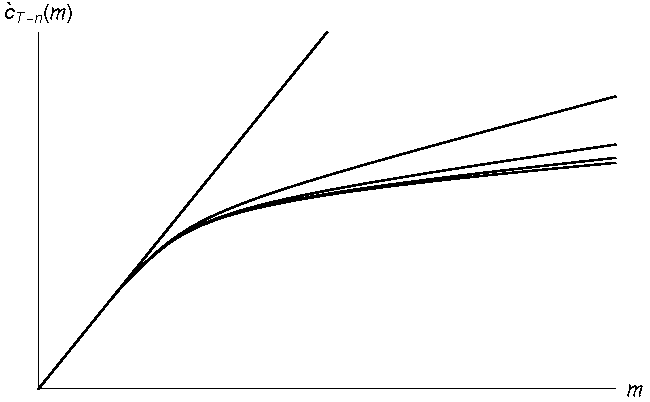
\includegraphics{./Figures/PlotCFuncsConverge}
  \caption{Converging $\Alt{\cFunc}_{T-n}({\mNrm})$ Functions as $n$ Increases}
  \label{fig:PlotCFuncsConverge}
\end{figure}


As an illustration, Figure \ref{fig:PlotCFuncsConverge} shows
$\Alt{\cFunc}_{T-n}({m})$ for $n=\{20,15,10,5,1\}$.  At least one
feature of this figure is encouraging: the consumption functions
converge as the horizon extends, something that \cite{BufferStockTheory}
shows must be true under certain parametric conditions that are
satisfied by the baseline parameter values being used here.


\Habits{
  \hypertarget{Multiple-State-Variables}{}
  \section{Multiple State Variables}
  We now wish to consider how the problem changes if there are multiple
  state variables rather than just a single state variable.  The example
  we will use will be the case where the utility from consumption
  depends on the size of a `habit stock' which represents an average of
  past levels of consumption.  Formally, the goal is to
  \begin{equation}
    \max \left\{ \sum_{s=t}^{T} \DiscFac^{s-t} \uFunc({c}_{s},h_{s-1}) \right\}
  \end{equation}
  Now there are two state variables in the problem at time $t$, the
  level of assets ${m}_{t}$ and the level of the habit stock $h_{t-1}$,
  where the accumulation equation for ${m}_{t}$ is the same as before and
  the transition equation for habits is
  \begin{equation}\begin{gathered}\begin{aligned}
        h_{t}  & = h_{t-1} + \MPS({c}_{t}-h_{t-1}).
      \end{aligned}\end{gathered}\end{equation}
  That is, the habit stock at the end of this period is equal to the
  habit stock at the end of last period plus a proportion of the gap
  between the level of consumption chosen this period and the level of
  the habit stock from last period.  In other words, habits `catch up'
  to consumption at rate $\MPS$.

  Assume that the utility function is given by
  \begin{equation}
    \uFunc({c}_{t},h_{t-1}) = \frac{({c}_{t}/h_{t-1}^{\gamma})^{1-\CRRA}}{1-\CRRA}.
  \end{equation}
  Now that $u_{t}$ has two arguments we need to be able to distinguish
  between the derivatives with respect to each argument.  Our notation
  will be that the derivative of $u_{t}$ with respect to ${c}_{t}$ is
  $u_{t}^{c}({c}_{t},h_{t-1})$ or $u_{t}^{c}$ for short, and analogously
  for $u_{t}^{h}$.  Thus we have
  \begin{equation}\begin{gathered}\begin{aligned}
        \uFunc^{c}_{t}  & = ({c}_{t} h_{t-1}^{-\gamma})^{-\CRRA}h_{t-1}^{-\gamma}  \\
        & = {c}_{t}^{-\CRRA}h_{t-1}^{\CRRA\gamma-\gamma}  \\
        \uFunc^{h}_{t}  & = -\gamma ({c}_{t} h_{t-1}^{-\gamma})^{-\CRRA} {c}_{t} h_{t-1}^{-\gamma-1} \\
        & = -\gamma {c}_{t}^{1-\CRRA}h_{t-1}^{\gamma\CRRA - \gamma -
          1} = -\gamma ({c}_{t}/h_{t-1}) \uFunc^{c}_{t}.
      \end{aligned}\end{gathered}\end{equation}

  Bellman's equation for this problem (imposing liquidity constraints again) is
  \begin{equation}\begin{gathered}\begin{aligned}
        {\vFunc}_{t}({m}_{t},h_{t-1})  & = \max_{\{{c}_{t}\}}  \{\uFunc({c}_{t},h_{t-1}) +
        \Ex_{t}[\DiscFac  {\vFunc}_{t+1}({m}_{t+1},h_{t}) ]\}
        \\ & \text{s.t.} & \nonumber \\
        {m}_{t+1}  & = [{m}_{t}-{c}_{t}]\RNrm_{t+1} + \TranShkEmp_{t+1}\\
        h_{t}  & = h_{t-1} + \MPS ({c}_{t} - h_{t-1} ) \\
        {c}_{t} & \leq  {m}_{t} .
      \end{aligned}\end{gathered}\end{equation}

  As was done for utility above, define the derivatives of ${\vFunc}_{t}$ with
  respect to each argument as ${\vFunc}_{t}^{m}({m}_{t},h_{t-1})$ (${\vFunc}_{t}^{m}$
  for short) and ${\vFunc}_{t}^{h}$.  Also as above, we want to
  define a function which corresponds to the expectation of the value of
  ending period $t$ in a given position, but now the `position'
  involves both the level of assets ${a}_{t}$ and the level of the habit
  stock $h_{t}$:
  \begin{equation}\begin{gathered}\begin{aligned}
        \vEndStget({a}_{t},h_{t})  & = \Ex_{t}[\DiscFac {v}_{t+1}(\RNrm_{t+1} {a}_{t}+{\TranShkEmp}_{t+1},h_{t}))]
      \end{aligned}\end{gathered}\end{equation}
  For future reference note that the derivatives are
  \begin{equation}\begin{gathered}\begin{aligned}
        \vEndStget^{{a}}  & = \DiscFac \Ex_{t} [\RNrm_{t+1} {v}_{t+1}^{m}] \label{eq:vEndsdefn} \\
        \vEndStget^{h}  & = \DiscFac \Ex_{t} [{\vFunc}_{t+1}^{h}] \label{eq:vEndhdefn}
      \end{aligned}\end{gathered}\end{equation}
  and the maximization problem can be rewritten
  \begin{equation}\begin{gathered}\begin{aligned}
        {\vFunc}_{t}({m}_{t},h_{t-1}) 
        & =                                         \max_{\{{c}_{t}\}} %\{
        \uFunc({c}_{t},h_{t-1})  +  \DiscFac
        \vEndStget({m}_{t}-{c}_{t},h_{t-1}+\MPS({c}_{t}-h_{t-1}))
        % \}
        \\        & \text{s.t.} & \nonumber
        \\  {c}_{t} & \leq  {m}_{t}.
      \end{aligned}\end{gathered}\end{equation}

  \hypertarget{The-Strategy}{}
  \subsection{The Strategy}

  This problem will be solved by a generalization of the strategy used
  to solve the one-state problem.  Previously, with a period-$t+1$
  consumption function in hand, we started by calculating
  $\vEndStget^{{a}}_{i}$ at the set of $n$ gridpoints ${a}_{i}$
  contained in the variable \texttt{aVec}.  Now we will need to
  have a grid of possible values for habits $h_{j}$ as well (in the
  variable \texttt{hVec}) with, say, $m$ gridpoints.  We will then
  calculate the values of $\vEndStget^{{a}}$ and $\vEndStget^{h}$
  at all \textit{combinations} of the ${a}_{i}$ and $h_{j}$
  gridpoints, for a total of $m \times n$ datapoints.  Finally, with
  these results in hand, we can obtain the corresponding values of
  consumption and construct the approximating interpolation to the
  consumption function.

  \hypertarget{Optimality-Conditions}{}
  \subsection{Optimality Conditions}
  \hypertarget{The-First-Orrder-Condition-for-c}{}
  \subsubsection{The First Order Condition for ${c}_{t}$}
  The FOC for this problem with respect to ${c}_{t}$ is:
  \ifthenelse{\boolean{MyNotes}}{\marginpar{\tiny The $-\MPS
      \vEndStget^{h}_{t}$ term reflects the fact that if you consume a
      bit more today, tomorrow's habit stock will be larger by $\MPS$,
      which will make you worse off.}}{}
  \begin{equation}\begin{gathered}\begin{aligned}
        0  & = \uFunc^{c}_{t} + \DiscFac \Ex_{t} \left[{\vFunc}^{m}_{t+1}(-\Rfree)+{\vFunc}^{h}_{t+1} \MPS\right]  \\
        \uFunc^{c}_{t}  & = \DiscFac \Ex_{t} [\RNrm_{t+1} {\vFunc}_{t+1}^{m}-\MPS {\vFunc}_{t+1}^{h}] \label{eq:ctfoc}
        \\            & = \left[\vEndStget^{{a}}-\MPS \vEndStget^{h} \right].
        % ({c}_{t}h_{t-1}^{-\gamma})^{-\CRRA}h_{t-1}^{-\gamma}  & = \DiscFac \Ex_{t} \left(\RNrm_{t+1} {\vFunc}^{m}_{t+1}-{\vFunc}^{h}_{t+1} \MPS\right) \label{eq:directfoc} \\
        % {c}_{t}^{-\CRRA}  & = h_{t-1}^{\gamma-\gamma\CRRA}\DiscFac \Ex_{t} \left(\RNrm_{t+1} {\vFunc}^{m}_{t+1}-{\vFunc}^{h}_{t+1} \MPS\right)
      \end{aligned}\end{gathered}\end{equation}
  Substituting the definition of $u_{t}^{c}$:
  \begin{equation}\begin{gathered}\begin{aligned}
        {c}_{t}^{-\CRRA}h_{t-1}^{\CRRA\gamma-\gamma}  & = \left[\vEndStget^{{a}}-\MPS \vEndStget^{h} \right]
        \\  {c}_{t}                                     & = \left[h_{t-1}^{\gamma-\CRRA\gamma} \left(\vEndStget^{{a}}-\MPS \vEndStget^{h} \right) \right]^{-1/\CRRA} \label{eq:habitsfoc}.
      \end{aligned}\end{gathered}\end{equation}
  and the liquidity constraint implies that if the $\check{c}_{t}$ which
  satisfies this equation is larger than ${m}_{t}$ the consumer spends
  ${m}_{t}$ rather than $\check{c}_{t}$.  The point at which the liquidity
  constraint becomes binding is therefore implicitly defined by the equation
  \begin{equation}\begin{gathered}\begin{aligned}
        {m}_{t}  & = \left[h_{t-1}^{\gamma-\CRRA\gamma} \left(\vEndStget^{{a}}(0,h_{t-1}+\MPS({m}_{t}-h_{t-1}))-\MPS \vEndStget^{h}(0,h_{t-1}+\MPS({m}_{t}-h_{t-1}))\right)  \right]^{-1/\CRRA}, \label{eq:LCbindsHabits}
      \end{aligned}\end{gathered}\end{equation}
  or incorporating the transition equation for
  and $h_{t-1}$ that
  \begin{equation}\begin{gathered}\begin{aligned}
        {c}_{t}  & = \left[h_{t-1}^{\gamma-\CRRA\gamma}
          \left(\vEndStget^{{a}}({m}_{t}-{c}_{t},h_{t-1}+\MPS({c}_{t}-h_{t-1}))
            -\MPS \vEndStget^{h}({m}_{t}-{c}_{t},h_{t-1}+\MPS({c}_{t}-h_{t-1})\right)
        \right]^{-1/\CRRA}. \nonumber
      \end{aligned}\end{gathered}\end{equation}

  This equation could be solved for a given grid of ${m}_{t}$ and
  $h_{t-1}$ values to yield the two-dimensional matrix of values
  necessary to construct an interpolating approximation to the
  consumption function.  However, note that the value of ${m}_{t}$ at
  which the constraint becomes binding depends on the level of
  $h_{t-1}$.  This causes a problem, because the built-in {\Mma}
  interpolation algorithms require multidimensional interpolations to
  contain a value for every possible combination of the independent
  variables.  Thus, we would need to add each of the $m$ binding
  points to the \texttt{mVec} variable, and to pair \textit{all} of
  those bindingpoints to \textit{each} possible value in \texttt{hVec}.
  This would immediately increase the number of points in the ${m}$
  dimension by $m$, so the total number of gridpoints would now be
  $(n+m) \times m$.  Thus this strategy would require increasing the
  size of the matrix of interpolating values by a \textit{factor} of $m$
  with a corresponding serious slowdown in computational speed.

  Fortunately, there is a way to get around this problem.  To
  understand it, start by noticing the translation in this context of
  the trick used to solve the one-dimensional consumption problem.
  Recall that there the trick was to start with the grid of values in
  \texttt{aVec} and find the unique ${\cNrm}_{i}$, and
  consequently ${m}_{i}={a}_{i}+{\cNrm}_{i}$, associated with
  each ${a}_{i}$ thus constructing the set of ${\cNrm}_{i}$ and
  ${m}_{i}$ values without solving a maximization problem or
  numerically finding a root.  Here, the most effective strategy is to
  use \texttt{aVec} to define a set of ${a}_{t}$ values but use
  \texttt{hVec} to define a set of values for $h_{t-1}$, with the
  transition equation determining the $h_{t}$ to be paired with the
  given ${a}_{t}$.  That is, defining the set $\mathcal{L} =
  \{\{{a}_{1},h_{1}\},\{{a}_{1},h_{2}\},\ldots,\{{a}_{m},h_{n_{\TranShkEmp}}\}\}$,
  we find the set of values of ${\cNrm}_{i}$ that satisfy
  \begin{equation}\begin{gathered}\begin{aligned}
        {\cNrm}_{k}^{\ell}  & = \left[(h_{k}^{\ell})^{\gamma-\CRRA\gamma}
          \left(\vEndStget^{{a}}({a}_{k}^{\ell},h_{k}^{\ell}
            +\MPS({\cNrm}_{k}^{\ell}-h_{k}^{\ell}))
            -\MPS
            \vEndStget^{h}({a}_{k}^{\ell},h_{k}^{\ell}+\MPS({\cNrm}_{k}^{\ell}-h_{k}^{\ell})\right)
        \right]^{-1/\CRRA}. \nonumber
      \end{aligned}\end{gathered}\end{equation}
  and the budget constraint again gives us the ${m}_{k}^{\ell}$
  associated with the given $\{{a}_{t},h_{t-1}\}$ pair.

  However, there is a problem: {\Mma}'s built-in two-dimensional
  interpolation routines require a complete set of values of ${c}_{t}$
  for \textit{each distinct} $\{{m}_{k},h_{j}\}$ pair.  But the list of
  ${m}_{k}$ gridpoints associated with each distinct point in
  \texttt{hVec} will be different.  Thus to use the built-in routines
  it would be necessary to take the union of all the ${m}_{k}$
  produced and then construct values of ${\cNrm}_{k}$ for each of
  these.  If there are $m$ values in \texttt{aVec}, this would
  mean solving the problem at a total of $m \times m \times n$
  girdpoints, only $m \times n$ of which would have been produced
  during the first-round procedure.

  There is a a much better solution: Manual interpolation.  This works
  as follows.  For each distinct value of $h_{t,i}$ the value of
  ${\cNrm}_{t,i}$ associated with each given ${a}_{t,i}$ is
  calculated as before, starting with ${a}_{1,t}=0$ which yields
  the value of ${m}_{t,i}$ and ${\cNrm}_{t,i}$ at which the
  constraint begins to bind for this combination of ${a}_{t,i}$
  and $h_{t,i}$.  Then an \texttt{InterpolatingFunction} is
  constructed as before.

  Thus we will have a collection of $j$ interpolating consumption
  functions, one for each value in \texttt{hVec}.  Denote these
  functions by $\Alt{\Hi{\cFunc}}_{t}({m}_{t},j)$.

  Now consider how to estimate $\cFunc_{t}({m}_{t},h_{t})$ for arbitrary
  ${m}_{t}$ and $h_{t}$.  Define $\underline{h}_{t}$ as the value, and
  $\underline{j}_{t}$ as the index of the nearest \texttt{hVec} point
  below $h_{t}$ and define $\bar{h}_{t}$ analogously for the nearest
  gridpoint above $h_{t}$.  Then we define our approximation to the
  consumption function as
  \begin{displaymath}
    \Alt{\Hi{\cFunc}}_{t}({m}_{t},h_{t}) =
    \Alt{\Hi{\cFunc}}({m}_{t},\underline{j})+\left(\frac{h_{t}-\underline{h}_{t}}
      {\bar{h}_{t}-\underline{h}_{t}}\right)
    \left(\Alt{\Hi{\cFunc}}({m}_{t},\overline{j})
      -\Alt{\Hi{\cFunc}}({m}_{t},\underline{j})\right)
  \end{displaymath}
  with points outside the \texttt{hVec} points constructed by
  extrapolation.

  Note that a liquidity constraint is again incorporated at almost
  zero cost: Simply make sure that the lowest value in
  \texttt{aVec} is 0, and append the point $\{0.,0.\}$ as the
  bottommost point in each of the lists of $\{{m}_{t},{c}_{t}\}$
  assoicated with the various values in \texttt{hVec}.

  \hypertarget{Applying-the-Envelope-Theorem}{}
  \subsubsection{Applying the Envelope Theorem}
  The Envelope theorem on ${m}_{t}$ says:
  \begin{equation}\begin{gathered}\begin{aligned}
        {\vFunc}^{m}_{t}  & = \frac{\partial {\vFunc}_{t}}{\partial {m}_{t}} + \overbrace{\frac{\partial {\vFunc}_{t}}{\partial {c}_{t}}}^{=0}\frac{\partial {c}_{t}}{\partial {m}_{t}} \label{eq:vxt} \\
        {\vFunc}_{t}^{m}  & = \DiscFac  \Ex_{t} [\RNrm_{t+1} {\vFunc}_{t+1}^{m}] \label{eq:envelopex}
      \end{aligned}\end{gathered}\end{equation}

  Substituting this into the FOC equation~(\ref{eq:ctfoc}) gives
  \begin{equation}\begin{gathered}\begin{aligned}
        \uFunc^{c}_{t}  & = {\vFunc}_{t}^{m}-\Ex_{t}[\DiscFac \MPS {\vFunc}_{t+1}^{h}] \label{eq:ctfocsubx}
        \\ {\vFunc}_{t}^{m}  & = \uFunc^{c}_{t}+\Ex_{t}[\DiscFac \MPS {\vFunc}_{t+1}^{h}] \label{eq:vtfoc}
        \\            & = \uFunc^{c}_{t}+\MPS \vEndStget^{h} \label{eq:vxtformula}.
      \end{aligned}\end{gathered}\end{equation}

  What if the consumer is liquidity constrained?  It is useful here to \ifthenelse{\boolean{MyNotes}}{\marginpar{\tiny By `is constrained' I mean the constraint is binding right now.}}{}
  rewrite Bellman's equation:
  \begin{equation}\begin{gathered}\begin{aligned}
        {\vFunc}_{t}({m}_{t},h_{t-1})  & = \uFunc({c}_{t},h_{t-1}) +  \DiscFac \Ex_{t}
        \left[{\vFunc}_{t+1}(({m}_{t}-{c}_{t})\RNrm_{t+1}+{\TranShkEmp}_{t+1},h_{t-1}+\MPS({c}_{t}-h_{t-1}))
        \right] \nonumber
      \end{aligned}\end{gathered}\end{equation}
  Substituting in the fact that ${c}_{t}={m}_{t}$ (because the consumer is constrained)
  \begin{equation}\begin{gathered}\begin{aligned}
        {\vFunc}_{t}({m}_{t},h_{t-1})  & = \uFunc({c}_{t},h_{t-1}) +  \Ex_{t}\left[\DiscFac
          {\vFunc}_{t+1}({\TranShkEmp}_{t+1},h_{t-1}+\MPS({c}_{t}-h_{t-1}))\right]
        \nonumber
      \end{aligned}\end{gathered}\end{equation}
  Thus $\partial {\vFunc}_{t}/\partial {m}_{t} = 0$, and because the liquidity
  constraint implies that $\partial {c}_{t}/\partial {m}_{t} = 1$,
  equation (\ref{eq:vxt}) becomes
  \begin{equation}\begin{gathered}\begin{aligned}
        {\vFunc}_{t}^{m}   & =  \frac{\partial {\vFunc}_{t}}{\partial {c}_{t}}
        \\              & = \uFunc_{t}^{c} + \DiscFac \Ex_{t} [\MPS {\vFunc}_{t+1}^{h}]
      \end{aligned}\end{gathered}\end{equation}
  which is identical to the expression (\ref{eq:vtfoc}) for ${\vFunc}_{t}^{m}$
  for the unconstrained consumer.

  The Envelope theorem for $h_{t-1}$ says:
  \begin{equation}\begin{gathered}\begin{aligned}
        {\vFunc}_{t}^{h}  & = \frac{\partial {\vFunc}_{t}}{\partial h_{t-1}} + \overbrace{\frac{\partial {\vFunc}_{t}}{\partial {c}_{t}}}^{=0}\frac{\partial {c}_{t}}{\partial h_{t-1}} \nonumber
        \\  & = \uFunc^{h}_{t} + \DiscFac \Ex_{t} \left[{\vFunc}_{t+1}^{h}\frac{\partial h_{t}}{\partial h_{t-1}} \right]\nonumber
        \\  & = \uFunc^{h}_{t} + \DiscFac \Ex_{t} [(1-\MPS) {\vFunc}_{t+1}^{h}] \nonumber
        \\  & = \uFunc^{h}_{t} + (1-\MPS) \vEndStget^{h} \label{eq:vhtformula}
      \end{aligned}\end{gathered}\end{equation}
  % & = -\gamma {c}_{t}^{1-\CRRA} h_{t-1}^{\gamma \CRRA - \gamma -1} + (1-\MPS) \DiscFac \Ex_{t} {\vFunc}_{t+1}^{h} \label{eq:vhtfoc}
  What if the consumer is constrained?  In that case while $\partial
  {\vFunc}_{t}/\partial {c}_{t} \neq 0$, $\partial {c}_{t}/\partial h_{t-1} = 0$, so as
  with ${\vFunc}_{t}^{m}$ the constraint has no effect on the expression for ${\vFunc}^{h}_{t}$.

  \hypertarget{Transforamtions}{}
  \subsection{Transformations}

  In the time-separable consumption problem, there was a unique
  transformation that allowed us to unwind much of the linearity
  attributable to the curvature of the utility function; this was
  possible because that problem has an analytical solution in the
  perfect foresight case, and because the problem is one with a single
  state variable.

  In the habits model, neither of these conditions is true, and
  consequently the appropriate transformation strategy is not obvious.
  To see this, consider the last period of life and suppose there is no
  uncertainty.  Then ${\vFunc}_{T}^{m} = \uFunc_{T}^{c}$ will be of the form
  ${c}_{T}^{-\CRRA}h_{T-1}^{\CRRA \gamma - \gamma}$, while ${\vFunc}_{T}^{h} =
  \uFunc^{h}$ will be something of the form $-\gamma
  {c}_{T}^{1-\CRRA}h_{T-1}^{\gamma\CRRA-\gamma-1}$.  It is possible to
  exponentiate either of these equations to make it linear in one or the
  other of ${c}$ or $h$, but not both.

  However, there is a two-step procedure that solves the problem.  In
  the first step, the object in question is transformed as in the
  original problem without habits.  For example, the transformed utility
  function for the last period of life would be
  \begin{equation}\begin{gathered}\begin{aligned}
        n_{T}^{c}  & = \left[\uFunc^{c}_{T}\right]^{-1/\CRRA}
        \\        & = {c}_{T}h_{T-1}^{\gamma(1/\CRRA-1)}.
      \end{aligned}\end{gathered}\end{equation}

  This leaves us with an equation that is linear in ${c}_{T}$ but
  nonlinear in $h_{T-1}$.  So now we do a second transformation:
  dividing the $n_{T}$ function by $h_{T-1}^{\gamma(1/\CRRA-1)}$.  This
  yields a function $\hat{n_{\TranShkEmp}}_{T}^{c}$ that can be transformed back into
  $\uFunc^{c}_{T}$ on demand, but is itself linear in ${c}_{t}.$  Analogously,
  in the last period of life the marginal value of habits is given by
  \begin{equation*}\begin{gathered}\begin{aligned}
        {\vFunc}_{T}^{h}  & = -\gamma {c}_{T}^{1-\CRRA}h_{T-1}^{\gamma(\CRRA-1)-1}
      \end{aligned}\end{gathered}\end{equation*}
  so the natural normalization procedure is to define
  \begin{equation}\begin{gathered}\begin{aligned}
        \Lambda_{t}^{h} 
        & =                           \left[\frac{h_{t-1}^{1-\gamma(\CRRA-1)}{\vFunc}_{t}^{h}}{-\gamma}\right]^{1/(1-\CRRA)}
      \end{aligned}\end{gathered}\end{equation}
  and similarly for $\vEndStget^{h}$.


  \hypertarget{Transforming-cFunc}{}
  \subsection{Transforming $\cFunc(\bullet,h_{t-1})$}

  The habits problem presents an additional difficulty: the consumption
  function is highly nonlinear in $h_{t-1}$ for a given ${m}_{t}$.   To
  see this, start with the first order condition for the problem in the
  second-to-last period of life (setting $\DiscFac = \RNrm_{t+1} = 1$ and assuming
  away uncertainty for transparency):
  \begin{equation}\begin{gathered}\begin{aligned}
        \uFunc_{t}^{c}    & = \uFunc_{t+1}^{c} - \MPS {\vFunc}_{t+1}^{h}
        \\      \uFunc_{T-1}^{c}  & = \uFunc_{T}^{c} - \MPS \uFunc_{T}^{h}
        \\   & =  \uFunc_{T}^{c}\left(1 + \gamma \MPS
          ({c}_{T}/h_{T-1})\right)
        \\      {c}_{T-1}^{-\CRRA} 
        & =                                      {c}_{T}^{-\CRRA}\left(\frac{h_{T-1}}{h_{T-2}}\right)^{\gamma(\CRRA-1)}\left(1 + \gamma \MPS
          ({c}_{T}/h_{T-1})\right)  \\
        {c}_{T-1} 
        & =                     ({m}_{T-1}-{c}_{T-1})\left(\frac{h_{T-1}}{h_{T-2}}\right)^{\gamma(1/\CRRA-1)}\left(1 +
          \gamma \MPS \left[\frac{{m}_{T-1}-{c}_{T-1}}{(1-\MPS)h_{T-2}+\MPS
              {c}_{T-1}}\right]\right)^{-1/\CRRA}
        \\      1 
        & =                     \left(\frac{{m}_{T-1}-{c}_{T-1}}{{c}_{T-1}}\right)\left(\frac{(1-\MPS)h_{T-2}+\MPS {c}_{T-1}}{h_{T-2}}\right)^{\gamma(1/\CRRA-1)}\left(1 +
          \gamma \MPS \left[\frac{{m}_{T-1}-{c}_{T-1}}{(1-\MPS)h_{T-2}+\MPS
              {c}_{T-1}}\right]\right)^{-1/\CRRA} \nonumber
        \\ \label{eq:oneeq}
      \end{aligned}\end{gathered}\end{equation}

  Now conjecture that for fixed ${m}_{T-1}$
  \begin{equation}
    \lim_{h_{T-1} \rightarrow 0} {c}_{T-1} = \mu h_{T-2}^{m}
    \label{eq:mueq}
  \end{equation}
  for some $\mu<1, \mu>1$.  Then the limit of \eqref{eq:oneeq} as $h_{T-2}
  \rightarrow \infty$ is given by
  \begin{equation*}\begin{gathered}\begin{aligned}
        1  & = ({m}_{T-1}/{c}_{T-1})\left(\frac{\MPS
            {c}_{T-1}}{h_{T-2}}\right)^{\gamma(1/\CRRA-1)}\left(\gamma
          \left[\frac{{m}_{T-1}}{{c}_{T-1}}\right]\right)^{-1/\CRRA}
        \\    
        & =                 {c}_{T-1}^{\gamma(1/\CRRA-1)-1+1/\CRRA}h_{T-2}^{-\gamma(1/\CRRA-1)}\MPS^{\gamma(1/\CRRA-1)}(\gamma {m}_{T-1})^{-1/\CRRA}
        \\    
        & =                 {c}_{T-1}^{(1+\gamma)(1/\CRRA-1)}h_{T-2}^{-\gamma(1/\CRRA-1)}\MPS^{\gamma(1/\CRRA-1)}(\gamma {m}_{T-1})^{-1/\CRRA}
        \\    
        & =                 {c}_{T-1}^{(1+\gamma)}h_{T-2}^{-\gamma}\MPS^{\gamma}(\gamma {m}_{T-1})^{1/(\CRRA-1)}
        \\ {c}_{T-1}    & = h_{T-2}^{\gamma/(1+\gamma)}\MPS^{-\gamma}(\gamma
        {m}_{T-1})^{\frac{1}{(\gamma+1)(\CRRA-1)}}
      \end{aligned}\end{gathered}\end{equation*}
  which confirms the conjecture \eqref{eq:mueq}.  On the other hand,
  suppose that we postulate that
  \begin{equation}
    \lim_{h_{T-2} \rightarrow \infty} {c}_{T-1} = \kappa.
    \label{eq:kappaguess}
  \end{equation}

  Under this conjecture, the limit of the RHS of \eqref{eq:oneeq} as
  $h_{T-2} \rightarrow \infty$ is
  \begin{equation*}\begin{gathered}\begin{aligned}
        \kappa 
        & =                  (1-\kappa)\left(1-\MPS\right)^{\gamma(1/\CRRA-1)}
        \\      \kappa\left(1+(1-\MPS)^{\gamma(1/\CRRA-1)}\right)  & = \left(1-\MPS\right)^{\gamma(1/\CRRA-1)}
        \\      \kappa 
        & =                          \left(\frac{\left(1-\MPS\right)^{\gamma(1/\CRRA-1)}}
          {1+(1-\MPS)^{\gamma(1/\CRRA-1)}}\right)
      \end{aligned}\end{gathered}\end{equation*}
  confirming conjecture \eqref{eq:kappaguess}.

  This combination of results indicates that the consumption function
  must be globally strongly nonlinear in $h_{T-1}$ (a nonlinearity which
  also arises in successive earlier periods $T-2$ and so on).

  If we wish to normalize the consumption rule by something that will
  help to make it approximately linear, that normalizing function will
  need approach proportionality to $h_{t-1}^{\gamma/(1+\gamma)}$ as
  $h_{t-1}$ goes to zero but approach a constant as $h_{t-1}$ approaches
  infinity.  The function
  \begin{equation}
    n(h_{t-1}) =
    h_{t-1}^{\gamma/(1+\gamma)}(h_{t-1}+\mu)^{-\gamma/(1+\gamma)}
  \end{equation}
  has precisely these characteristics for $\mu>0$.  Some
  experimentation with possible values of $\mu$ led to the conclusion
  that under the baseline parameter values this function does a good job
  of linearizing the relationship between consumption and $h_{t-1}$ for
  a value of $\mu = 0.04$.

  The combined transformations for the various variables are thus
  \begin{equation}\begin{gathered}\begin{aligned}
        \cFunc_{\overline{t}}^{{a}}({a}_{t},h_{t})        & = [\vEndStget^{{a}}({a}_{t},h_{t})]^{-1/\CRRA} h_{t}^{\gamma(1-1/\CRRA)} \label{eq:vEndstransform} \\
        \Lambda_{t}^{m}({m}_{t},h_{t-1})   & = [{\vFunc}_{t}^{m}({m}_{t},h_{t-1})]^{-1/\CRRA} h_{t-1}^{\gamma(1-1/\CRRA)} \label{eq:vxtransform} \\
        \cFunc_{\overline{t}}^{h}({a}_{t},h_{t})       
        & =                                                  [-h_{t}^{1-\gamma(\CRRA-1)}\vEndStget^{h}({a}_{t},h_{t})/\gamma]^{1/(1-\CRRA)}  \label{eq:vEndhtransform}
        \\      \Lambda_{t}^{h}({m}_{t},h_{t-1})   & = [-h_{t-1}^{1-\gamma(\CRRA-1)}{\vFunc}_{t}^{h}({m}_{t},h_{t-1})/\gamma]^{1/(1-\CRRA)} \label{eq:vhtransform}
        \\      \Lambda_{t}({m}_{t},h_{t-1})       & = [(1-\CRRA)
        {\vFunc}_{t}({m}_{t},h_{t-1})]^{1/(1-\CRRA)} h_{t-1}^{\gamma}\label{eq:vtransform}
        \\  \chi({m}_{t},h_{t-1})       & = \cFunc({m}_{t},h_{t-1})h_{t-1}^{-\gamma/(1+\gamma)}(h_{t-1}+\mu)^{\gamma/(1+\gamma)}.
      \end{aligned}\end{gathered}\end{equation}
  where these are the functions that are actually approximated by
  interpolation and the objects of interest (like the consumption
  function) are obtained by reversing the transformations.

  \hypertarget{The-Program}{}
  \subsection{The Program}
  The consumption problem with habit formation is solved in
  \texttt{habits.m}, whose structure closely follows that of
  \texttt{multiperiod.m}.

  Assuming the problem has been solved up to period $t+1$ (and thus we
  have numerical functions $\hat{\vFunc}_{t+1}^{m}({m}_{t+1},h_{t})$ and
  $\hat{\vFunc}_{t+1}^{h}({m}_{t+1},h_{t})$),
  \begin{enumerate}

  \item Form a list called \texttt{ArgArray} of all possible
    combinations of the values in \texttt{aVec} and
    \texttt{hVec}, and index the components of that list by $k$.  Thus
    if there are $m$ points in both grids we have \texttt{ArgArray}=
    $\{\{{a}_{1},h_{1}\}$, $\{{a}_{1},h_{2}\},\ldots$,
    $\{{a}_{1},h_{m}\}$, $\{{a}_{2},h_{1}\}$,
    $\{{a}_{2},h_{2}\},\ldots$, $\{{a}_{2},h_{m}\},
    \{{a}_{m},h_{1}\}$, $\{{a}_{m},h_{2}\},\ldots$,
    $\{{a}_{m},h_{m}\}\}$.  Designate this list as $\mathcal{L}$
    with individual members $\{\ell_{1}, \ell_{2}, \ldots \ell_{m \times
      m}\}$.  Finally, define the notation $\bullet^{\ell}_{k}$ to mean
    ``the value of $\bullet$ associated with the $k$th element of the
    list $\mathcal{L}$; e.g. $h^{\ell}_{1} = h_{1}$, $h^{\ell}_{2} =
    h_{2}$, and ${a}^{\ell}_{2}={a}_{1}$.''

    Now at each of the $k$ locations in \texttt{ArgArray} calculate the
    value of $\cFunc_{\overline{t}}^{{a}}$ and $\cFunc_{\overline{t}}^{h}$ (from
    equations (\ref{eq:vEndsdefn}) and (\ref{eq:vEndhdefn})) and
    \eqref{eq:vEndstransform} and \eqref{eq:vEndhtransform},
    \begin{equation}\begin{gathered}\begin{aligned}
          \cEndFunc_{k,t}^{{a}}  & = (h_{k}^{\ell})^{\gamma(1-1/\CRRA)}
          \left(\DiscFac \Ex_{t}
            \left[
              \RNrm_{t+1} (\hat{\vFunc}_{t+1}^{m}(\RNrm_{t+1} s^{\ell}_{k} +
              {\TranShkEmp}_{t+1},h^{\ell}_{k}))
            \right]
          \right)^{-1/\CRRA}
          \\      \cEndFunc_{k,t}^{h} 
          & =                                         \left(-(h_{k}^{\ell})^{1-\gamma(\CRRA-1)} \DiscFac \Ex_{t}
            \left[
              \hat{\vFunc}_{t+1}^{h}(\RNrm_{t+1} s^{\ell}_{k} +
              {\TranShkEmp}_{t+1},h^{\ell}_{k})
            \right]/\gamma
          \right)^{1/(1-\CRRA)},
        \end{aligned}\end{gathered}\end{equation}
    generating lists of values
    $\cEndFunc^{a}_{k,t}$,$\cEndFunc^{h}_{k,t}$.

  \item Construct interpolating functions $\hat{\cEndFunc}^{a}_{t}({a}_{t},h_{t})$
    and $\hat{\cEndFunc}^{h}_{t}({a}_{t},h_{t})$, from which we can
    obtain $\hat{\vEndStget}^{a}_{t}$ and $\hat{\vEndStget}^{h}_{t}$
    via the inverse of the transformations (\ref{eq:vEndstransform})
    and (\ref{eq:vEndhtransform}).

  \item Loop over the $m$ values of $h$ in \texttt{hVec}, indexing them
    by $j$; for each $j$:
    \begin{itemize}
    \item Loop over ${a}_{i}$ finding the optimal ${c}_{a}$ associated
      with this ${a}_{i}$ and $h_{j}$ from the formula in equation
      \eqref{eq:habitsfoc}:
      \begin{equation}
        {\cNrm}_{i} = \left[h_{j}^{\gamma-\CRRA \gamma}
          (\vEndStget^{{a}}({a}_{i},(1-\MPS) h_{j}+ {\cNrm}_{i})
          -\MPS \vEndStget^{h}({a}_{i},(1-\MPS)
          h_{j}+{\cNrm}_{i}))\right]^{-1/\CRRA} \nonumber
      \end{equation}

    \item Construct ${m}_{i} = {\cNrm}_{i}+{a}_{i}$

    \item Construct \texttt{ct[mt,j]} as a linear interpolation of the
      $\{{m}_{i},{\cNrm}_{i}\}$
    \end{itemize}
  \end{enumerate}

  With $\Alt{\Hi{\cFunc}}_{t}({m}_{t},h_{t-1})$, $\hat{\vEndStget}^{{a}}$
  and $\hat{\vEndStget}^{h}$ in hand we can obtain ${\vFunc}^{m}_{t}$
  and ${\vFunc}^{h}_{t}$ from \eqref{eq:vxtformula} and
  \eqref{eq:vhtformula}. Thus we have generated $\Alt{\Hi{\cFunc}}_{t}$,
  $\hat{\vFunc}^{m}_{t}$ and $\hat{\vFunc}^{h}_{t}$ from $\hat{\vFunc}^{a}_{t+1}$ and
  $\hat{\vFunc}^{h}_{t+1}$, and we can continue the iteration indefinitely.

  The problem is solved in the program \texttt{habits.m}.  Details of
  the {\Mma}~implementation follow those described above for
  \texttt{multiperiod.m} closely, and so need not be described here.
  The program generates a three-D figure showing the consumption rule
  $\cFunc_{t}({m}_{t},h_{t-1})$ for the first period of `life.'  The figure
  behaves as one would expect: consumption is increasing in the level
  of resources and in the level of the habit stock.\footnote{For a
    detailed analysis of some of the properties of this habit formation
    model, see Carroll~\citeyearpar{carroll:RiskyHabits}}


}{}

\hypertarget{Multiple-Control-Variables}{}
\section{Multiple Control Variables}

We now consider how to solve problems with multiple control variables.
(To reduce notational complexity, in this section we set $\PermGroFac_{t}=1~\forall~t$.)

\subsection{Theory}
The new control variable that the consumer can now choose is the portion of the portfolio to invest in risky assets.  Designating the gross return on the risky asset as $\Risky_{t+1}$, and using $\varsigma_{t}$ to represent the proportion of the portfolio invested in this asset before the return is realized after the beginning of $t+1$, corresponding to an assumption that the consumer cannot be `net short' and cannot issue net equity), the overall return on the consumer's portfolio between $t$ and $t+1$ will be:
\begin{verbatimwrite}{./Equations/Rport.tex}
  \begin{equation}\begin{gathered}\begin{aligned}
        \Rport_{t+1}  & = \Rfree(1-\varsigma_{t}) + \Risky_{t+1}\varsigma_{t} \label{eq:return1}
        \\               & = \Rfree + (\Risky_{t+1}-\Rfree) \varsigma_{t} %\label{eq:return2}
      \end{aligned}\end{gathered}\end{equation}
\end{verbatimwrite}
  \begin{eqnarray}
    \Rport_{t+1} & = & \Rfree(1-\varsigma_{t}) + \Risky_{t+1}\varsigma_{t} \label{eq:return1}
    \\              & = & \Rfree + (\Risky_{t+1}-\Rfree) \varsigma_{t} \label{eq:return2}
  \end{eqnarray}
\unskip
and the maximization problem is
\begin{verbatimwrite}{./Equations/PortProb.tex}
  \begin{equation*}\begin{gathered}\begin{aligned}
        {\vFunc}_{t}({m}_{t})  & = \max_{\{{c}_{t},\varsigma_{t}\}}   ~~ \uFunc({c}_{t}) +  \DiscFac
        \Ex_{t}[{\vFunc}_{t+1}({m}_{t+1})]
        \\      & \text{s.t.} & \nonumber
        \\      \Rport_{t+1}  & = \Rfree + (\Risky_{t+1}-\Rfree) \varsigma_{t}
        \\      {m}_{t+1}  & = ({m}_{t}-{c}_{t})\Rport_{t+1} + \TranShkEmp_{t+1}
        \\  0       \leq & \varsigma_{t}  \leq 1, \label{eq:noshorts}
      \end{aligned}\end{gathered}\end{equation*}
\end{verbatimwrite}
  \begin{equation*}\begin{gathered}\begin{aligned}
    {\vFunc}_{t}({m}_{t})  & = \max_{\{{c}_{t},\varsigma_{t}\}}   ~~ \util({c}_{t}) +  \Discount
                                \Ex_{t}[{\vFunc}_{t+1}({m}_{t+1})]
    \\      & \text{s.t.} &
    \\      \Rport_{t+1}  & = \Rfree + (\Risky_{t+1}-\Rfree) \varsigma_{t}
    \\      {m}_{t+1}  & = ({m}_{t}-{c}_{t})\Rport_{t+1} + \tShkEmp_{t+1}
    \\  0       \leq & \varsigma_{t} & \leq 1, \label{eq:noshorts}
  \end{aligned}\end{gathered}\end{equation*}
\unskip
or, more compactly,
\begin{equation*}\begin{gathered}\begin{aligned}
      {\vFunc}_{t}({m}_{t})  & = \max_{\{\cFunc_{t},\varsigma_{t}\}} ~~  \uFunc({c}_{t}) +  \Ex_{t}[\DiscFac {\vFunc}_{t+1}(({m}_{t}-{c}_{t}){\Rport}_{t+1} +        {\TranShkEmp}_{t+1})]
      \\                       & \text{s.t.} & \nonumber
      \\ 0 \leq & \varsigma_{t} \leq 1
      .
    \end{aligned}\end{gathered}\end{equation*}
The first order condition with respect to ${c}_{t}$ is almost identical
to that in the single-control problem, equation (\ref{eq:upceqEvtp1}),
with the only difference being that the nonstochastic interest factor
$\Rfree$ is now replaced by ${\Rport}_{t+1}$,
\begin{verbatimwrite}{./Equations/valfuncFOCRtilde.tex}
  \begin{equation}\begin{gathered}\begin{aligned}
        \uFunc^{{c}}({c}_{t})  & = \DiscFac \Ex_{t} [{\Rport}_{t+1} \vFunc^{{m}}_{t+1}({m}_{t+1})] \label{eq:valfuncFOCRtilde},
      \end{aligned}\end{gathered}\end{equation}
\end{verbatimwrite}
  \begin{equation}\begin{gathered}\begin{aligned}
        \uFunc^{{c}}({c}_{t})  & = \DiscFac \Ex_{t} [{\Rport}_{t+1} \vFunc^{{m}}_{t+1}({m}_{t+1})] \label{eq:valfuncFOCRtilde},
      \end{aligned}\end{gathered}\end{equation}
\unskip
and the Envelope theorem derivation remains the same, 
yielding the Euler equation for consumption
\begin{verbatimwrite}{./Equations/EulercRiskyR.tex}
  \begin{equation}\begin{gathered}\begin{aligned}
        \uFunc^{{c}}({c}_{t})  & = \Ex_{t}[\DiscFac {\Rport}_{t+1} \uFunc^{{c}}({c}_{t+1})]. \label{eq:EulercRiskyR}
      \end{aligned}\end{gathered}\end{equation}
\end{verbatimwrite}
  \begin{equation}\begin{gathered}\begin{aligned}
        \uFunc^{{c}}({c}_{t})  & = \Ex_{t}[\DiscFac {\Rport}_{t+1} \uFunc^{{c}}({c}_{t+1})]. \label{eq:EulercRiskyR}
      \end{aligned}\end{gathered}\end{equation}
\unskip

The first order condition with respect to the risky portfolio share is
\begin{verbatimwrite}{./Equations/FOCw.tex}
  \begin{equation}\begin{gathered}\begin{aligned}
        0  & = \Ex_{t}[{\vFunc}_{t+1}^{{m}}({m}_{t+1})(\Risky_{t+1}-\Rfree){a}_{t}] \notag
        \\         & = {a}_{t}\Ex_{t}\left[\uFunc^{{c}}\left(\cFunc_{t+1}({m}_{t+1})\right)(\Risky_{t+1}-\Rfree)\right] \label{eq:FOCw}.
      \end{aligned}\end{gathered}\end{equation}
\end{verbatimwrite}
  \begin{equation}\begin{gathered}\begin{aligned}
    0  & = \Ex_{t}[{\vFunc}_{t+1}^{\prime}({m}_{t+1})(\Risky_{t+1}-\Rfree){a}_{t}]
    \\         & = {a}_{t}\Ex_{t}\left[\util^{\prime}\left(\cFunc_{t+1}({m}_{t+1})\right)(\Risky_{t+1}-\Rfree)\right] \label{eq:FOCw}.
  \end{aligned}\end{gathered}\end{equation}
\unskip

As before, it will be useful to define $\vEndStget$ as a function that
yields the expected $t+1$ value of ending period $t$ in a given state.
However, now that there are two control variables, the expectation
must be defined as a function of the chosen values of both of those
variables, because expected end-of-period value will depend not just
on how much the agent saves, but also on how the saved assets are
allocated between the risky and riskless assets.  Thus we define
\begin{equation*}\begin{gathered}\begin{aligned}
      \vEndStget({a}_{t},\varsigma_{t})  & = \Ex_{t}[\DiscFac {\vFunc}_{t+1}({m}_{t+1})]
    \end{aligned}\end{gathered}\end{equation*}
which has derivatives
\begin{equation}\begin{gathered}\begin{aligned}
      \vEndStget^{{a}}  & = \Ex_{t}[\DiscFac {\Rport}_{t+1}{\vFunc}_{t+1}^{m}({m}_{t+1})] = \Ex_{t}[\DiscFac {\Rport}_{t+1}{\uFunc}_{t+1}^{{c}}(\cFunc_{t+1}({m}_{t+1}))]
      \\      \vEndStget^{\varsigma}  & = \Ex_{t}[\DiscFac (\Risky_{t+1}-\Rfree){\vFunc}_{t+1}^{m}({m}_{t+1})  ]a_{t} = \Ex_{t}[\DiscFac (\Risky_{t+1}-\Rfree){\uFunc}_{t+1}^{{c}}(\cFunc_{t+1}({m}_{t+1}))  ]a_{t} \notag
    \end{aligned}\end{gathered}\end{equation}
implying that the first order conditions (\ref{eq:EulercRiskyR}) and
(\ref{eq:FOCw}) can be rewritten
\begin{equation}\begin{gathered}\begin{aligned}
      \uFunc^{{c}}({c}_{t})  & = \vEndStget^{{a}}({m}_{t}-{c}_{t},\varsigma_{t})
      \\      0  & = \vFunc^{\varsigma}_{\overline{t}}({a}_{t},\varsigma_{t}).
    \end{aligned}\end{gathered}\end{equation}

\subsection{Application}

Our first step is to specify the stochastic process for $\Risky_{t+1}$.
We follow the common practice of assuming that returns are
lognormally distributed, $\log \Risky \sim
\mathcal{N}(\eprem+\rfree-\sigma^{2}_{\eprem}/2,\sigma^{2}_{\eprem})$ where $\eprem$ is the equity premium
over the returns $\rfree$ available on the riskless asset.\footnote{This guarantees that $\Ex[\Risky] = \EPrem$ is invariant to the choice of $\sigma^{2}_{\eprem}$; see \handoutM{LogELogNorm}.}

As with labor income uncertainty, it is necessary to discretize the
rate-of-return risk in order to have a problem that is soluble in a
reasonable amount of time.  We follow the same procedure as for labor
income uncertainty, generating a set of $n_{\risky}$ equiprobable shocks to the
rate of return; in a slight abuse of notation, we will designate
the portfolio-weighted return (contingent on the
chosen portfolio share in equity, and potentially contingent on any other
aspect of the consumer's problem) simply as $\Rport_{i,j}$ (where dependence
on $i$ is allowed to permit the possibility of nonzero correlation
between the return on the risky asset and the shock to labor income (for example,
in recessions the stock market falls and labor income also declines).

The direct expressions for the derivatives of $\vEndStget$ are
\begin{equation}\begin{gathered}\begin{aligned}
      \vEndStget^{{a}}({a}_{t},\varsigma_{t})  & = \DiscFac \left(\frac{1}{n_{\risky} n_{\TranShkEmp}}\right)\sum_{i=1}^{n_{\TranShkEmp}}\sum_{j=1}^{n_{\risky} }\Rport_{i,j} \left(\cFunc_{t+1}(\Rport_{i,j}{a}_{t}+\TranShkEmp_{i})\right)^{-\CRRA}
      \\      \vEndStget^{\varsigma}({a}_{t},\varsigma_{t})  & = \DiscFac \left(\frac{1}{n_{\risky} n_{\TranShkEmp}}\right)\sum_{i=1}^{n_{\TranShkEmp}}\sum_{j=1}^{n_{\risky} }(\Risky_{i,j}-\Rfree)\left(\cFunc_{t+1}(\Rport_{i,j}{a}_{t}+\TranShkEmp_{i})\right)^{-\CRRA}.
    \end{aligned}\end{gathered}\end{equation}

Writing these equations out explicitly makes a problem very
apparent: For every different combination of $\{{a}_{t},\varsigma_{t}\}$
that the routine wishes to consider, it must perform two
double-summations of $n_{\risky} \times n$ terms.  Once again, there is an
inefficiency if it must perform these same calculations many times
for the same or nearby values of $\{{a}_{t},\varsigma_{t}\}$, and again
the solution is to construct an approximation to the derivatives of
the $\vEndStget$ function.

Details of the construction of the interpolating approximation are
given below; assume for the moment that we have the approximations
$\hat{\vEndStget}^{{a}}$ and $\hat{\vEndStget}^{\varsigma}$ in
hand and we want to proceed.  As noted above, nonlinear equation
solvers (including those built into {\Mma}) can find the
solution to a set of simultaneous equations.  Thus we could ask
{\Mma}~to solve
\begin{equation}\begin{gathered}\begin{aligned}
      {c}_{t}^{-\CRRA}  & = \hat{\vFunc}^{a}_{\overline{t}}({m}_{t}-{c}_{t},\varsigma_{t}) %\label{eq:FOCwrtcMultContr}
      \\      0  & = \hat{\vFunc}^{\varsigma}_{\overline{t}}({m}_{t}-{c}_{t},\varsigma_{t}) \label{eq:FOCwrtw}
    \end{aligned}\end{gathered}\end{equation}
simultaneously for $\cNrm$ and $\varsigma$ at the set of potential ${m}_{t}$ values defined in
\texttt{mVec}. However, multidimensional constrained
maximization problems are difficult and sometimes quite slow to
solve.  There is a better way.  Define the problem
\providecommand{\Opt}{}
\renewcommand{\Opt}{\tilde}
\providecommand{\vOpt}{}
\renewcommand{\vOpt}{\overset{*}{\vFunc}}
\begin{equation}\begin{gathered}\begin{aligned}
      \Opt{\vFunc}_{\overline{t}}({a}_{t})  & = \max_{\varsigma_{t}} ~~  \vEndStget({a}_{t},\varsigma_{t})
      \\      & \text{s.t.} & \nonumber
      \\      0 \leq & \varsigma_{t} \leq 1
    \end{aligned}\end{gathered}\end{equation}
where the tilde over $\Opt{\vFunc}(a)$ indicates that this is the $\vFunc$ that has been optimized with
respect to all of the arguments other than the one still present
(${a}_{t}$).  We solve this problem for the set of gridpoints in
\texttt{aVec} and use the results to construct the interpolating
function $\Alt{\Opt{\vFunc}}_{t}^{a}({a}_{t})$.\footnote{A faster solution
  could be obtained by, for each element in \texttt{aVec}, computing
  $\vEndStget^{\varsigma}({m}_{t}-{c}_{t},\varsigma)$ of a grid of
  values of $\varsigma$, and then using an approximating interpolating
  function (rather than the full expectation) in the \texttt{FindRoot}
  command.  The associated speed improvement is fairly modest,
  however, so this route was not pursued.}  With this function in
hand, we can use the first order condition from the single-control
problem
\begin{equation*}\begin{gathered}\begin{aligned}
      {c}_{t}^{-\CRRA}  & = \Alt{\Opt{\vFunc}}_{t}^{{a}}({m}_{t}-{c}_{t})
    \end{aligned}\end{gathered}\end{equation*}
to solve for the optimal level of consumption as a function of
${m}_{t}$ using the endogenous gridpoints method described above.  Thus we have transformed the multidimensional optimization
problem into a sequence of two simple optimization problems.

Note the parallel between this trick and the fundamental insight of
dynamic programming: Dynamic programming techniques transform a
multi-period (or infinite-period) optimization problem into a sequence
of two-period optimization problems which are individually much easier
to solve; we have done the same thing here, but with multiple dimensions
of controls rather than multiple periods.

\hypertarget{Implementation}{}
\subsection{Implementation}

The program which solves the constrained problem with multiple control variables
is \texttt{multicontrolCon.m}.

Some of the functions defined in \texttt{multicontrolCon.m} correspond
to the derivatives of $\vEndStget({a}_{t},\varsigma_{t})$.
\ifhabits{Structurally these functions are very similar to the
  $\vEndStget({a}_{t},h_{t})$ functions defined in
  \texttt{habits.m}; indeed, from the standpoint of the end of period
  $t$ after the portfolio share has been chosen, the portfolio share
  is essentially a state variable, so the resemblance to the
  multistate problem is more than skin deep.}{}

The first function definition that does not resemble anything in\ifhabits{ either \texttt{habits.m} or}{} \texttt{multiperiod.m} is
\texttt{$\riskyshare$Raw[at\_]}. This function, for its input value of
${a}_{t}$, calculates the value of the portfolio share $\varsigma_{t}$
which satisfies the first order condition (\ref{eq:FOCwrtw}), tests
whether the optimal portfolio share would violate the constraints,
and if so resets the portfolio share to the constrained optimum. The
function returns the optimal value of the portfolio share itself,
$\varsigma_{t}^{*}$, from which the functions
$\bar{\vEndStget}^{a}({a}_{t})$ and $\hat{\varsigma}_{t}({a}_{t})$ will be
constructed.

As $\hat{\varsigma}_{t}({a}_{t})$ can be constructed by
\texttt{$\riskyshare$Raw[at\_]}, $\bar{\vEndStget}^{a}({a}_{t})$ is
constructed by another newly defined function
\texttt{vEndStgetaOpt[at\_]}, where the naming convention is obviously
that `Opt' stands for `Optimized.' With
$\bar{\vEndStget}^{{a}}({a}_{t})$ in
hand (as well as the appropriately redefined
$\bar{\vEndStget}({a}_{t})$ and $\bar{\vEndStget}^{{aa}}({a}_{t})$) the analysis is essentially identical to that for the standard
multiperiod problem with a single control variable.

The structure of the program in detail is as follows.  First,
perform \ifthenelse{\boolean{MyNotes}}{\marginpar{\tiny Note choice
    of $\CRRA=10$ to match stockholding puzzle.}}{} the usual
initializations. Then initialize \texttt{$\riskyshare$Vec} and the other
variables specific to the multiple control problem.\footnote{Note
  the choice of a coefficient of relative risk aversion of 6, in
  contrast with the choice of 2 made for the previous problems.  This
  choice reflects the well-known `stockholding puzzle,' which is the
  microeconomic equivalent of the equity premium puzzle: For plausible
  descriptions of income uncertainty, rate of return risk, and the
  equity premium, the typical consumer should hold all or nearly all
  of their portfolio in equities. Thus we choose a high value for the
  coefficient of relative risk aversion in order to generate portfolio
  structure behavior more interesting than a choice of 100 percent
  equities in every period for every level of wealth.} In particular,
there are now three kinds of functions: those with both ${a}_{t}$
and $\varsigma_{t}$ as arguments, those with just ${a}_{t}$, and those
with ${m}_{t}$.

Once the setup is complete, the heart of the program is the
following.

\begin{enumerate}

\item Construct
  $\vEndStget^{\varsigma}({a}_{t},\varsigma_{t})$ using the usual calculation
  over the tensor defined by the combinations of the elements of
  \texttt{aVec} and \texttt{$\riskyshare$Vec}.

\item For any level of saving \texttt{at}, the function \texttt{$\riskyshare$Raw[at\_]} performs a rootfinding
  operation\footnote{Alternatively, the rootfinding operation would be
    $0 = \hat{\vFunc}^{\varsigma}_{\overline{t}}({a}_{t},\varsigma_{t})$, where the
    interpolation function of $\vEndStget^{\varsigma}({a}_{t},\varsigma_{t})$ is
    used instead. However, the results obtained (especially
    $\hat{\varsigma}_{t}({a}_{t})$) are much less satisfactory.}
  \begin{equation}\begin{gathered}\begin{aligned}
        0  & = \vFunc^{\varsigma}_{\overline{t}}({a}_{t},\varsigma_{t})
        \\      & \text{s.t.} & \nonumber
        \\      0 \leq & \varsigma_{t}  \leq 1
      \end{aligned}\end{gathered}\end{equation}
  and generates the corresponding optimal portfolio share
  $\varsigma^{\ast}_{t}$.

\item Construct the function \texttt{$\Opt{\vFunc}$a[at\_]}
  \begin{equation}\begin{gathered}\begin{aligned}
        \Opt{\vFunc}_{t}^{a}({a}_{t}) \equiv
        \vEndStget^{a}({a}_{t},\varsigma^{\ast}_{t}({a}_{t}))
      \end{aligned}\end{gathered}\end{equation}
  where $\varsigma^{\ast}_{t}({a}_{t})$ is computed by \texttt{$\riskyshare$Raw[at\_]}.

\item Using $\Opt{\vFunc}_{t}^{a}({a}_{t}) \equiv$
  \texttt{$\Opt{\vFunc}$a[at\_]} and the redefined
  $\Opt{\vFunc}_{t}({a}_{t})$ and $\Opt{\vFunc}_{t}^{{aa}}({a}_{t})$ (in
  place of $\vEndStget^{a}({a}_{t}) \equiv $ \texttt{vEndStgeta[at\_]} in
  \texttt{multiperiod.m}), follow the same procedures as in
  \texttt{multiperiod.m} to generate $\Alt{\cFunc}_{t}({m})$.

\end{enumerate}

\
\subsection{Results}

Figure~\ref{fig:PlotctMultContr} plots the first-period consumption
function generated by the program; qualitatively it does not look much
different from the consumption functions generated by the program
without portfolio choice.  Figure~\ref{fig:PlotRiskySharetOfat} plots the
optimal portfolio share as a function of the level of assets.  This
figure exhibits several interesting features.  First, even with a
coefficient of relative risk aversion of 6, an equity premium of only
4 percent, and an annual standard deviation in equity returns of 15
percent, the optimal choice is for the agent
to invest a proportion 1 (100 percent) of the portfolio in stocks (instead of the safe bank account with riskless return $\Rfree$) is
at values of ${a}_{t}$ less than about 2.  Second, the
proportion of the portfolio kept in stocks is \textit{declining} in the
level of wealth - i.e., the poor should hold all of their meager
assets in stocks, while the rich should be cautious, holding more of
their wealth in safe bank deposits and less in stocks.  This
seemingly bizarre (and highly counterfactual) prediction reflects the
nature of the risks the consumer faces.  Those consumers who are poor
in measured financial wealth are likely to derive a high proportion of
future consumption from their labor income.  Since by assumption labor
income risk is uncorrelated with rate-of-return risk, the covariance
between their future consumption and future stock returns is
relatively low.  By contrast, persons with relatively large wealth
will be paying for a large proportion of future consumption out of that
wealth, and hence if they invest too much of it in stocks their consumption
will have a high covariance with stock returns.  Consequently, they
reduce that correlation by holding some of their wealth in the
riskless form.

\hypertarget{PlotctMultContr}{}
\begin{figure}
  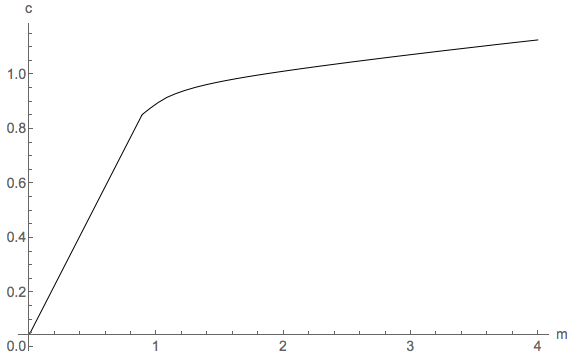
\includegraphics{./Figures/PlotctMultContr}
  \caption{$\cFunc({m}_{1})$ With Portfolio Choice}
  \label{fig:PlotctMultContr}
\end{figure}

\hypertarget{PlotRiskySharetOfat}{}
\begin{figure}
  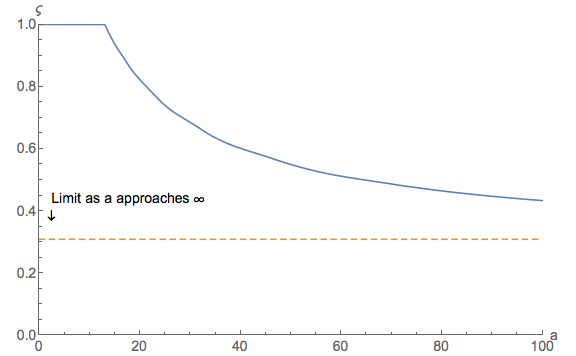
\includegraphics{./Figures/PlotRiskySharetOfat}
  \caption{Portfolio Share in Risky Assets in First Period $\varsigma({a})$}
  \label{fig:PlotRiskySharetOfat}
\end{figure}

\hypertarget{The-Infinite-Horizon}{}
\section{The-Infinite-Horizon}

All of the solution methods presented so far have involved
period-by-period iteration from an assumed last period of life, as is
appropriate for life cycle problems.  However, if the parameter values
for the problem satisfy certain conditions (detailed in
\cite{BufferStockTheory}), the consumption rules (and the rest of
the problem) will converge to a fixed rule as the horizon (remaining
lifetime) gets large, as illustrated in
Figure~\ref{fig:PlotCFuncsConverge}.  Furthermore,
Deaton~\citeyearpar{deatonLiqConstr},
Carroll~\citeyearpar{carroll:brookings,carrollBSLCPIH} and others
have argued that the `buffer-stock' saving behavior that emerges under
some further restrictions on parameter values is a good approximation
of the behavior of typical consumers over much of the lifetime.
Methods for finding the converged functions are therefore of interest,
and are dealt with in this section.

Of course, the simplest such method is to solve the problem as
specified above for a large number of periods.  This is feasible, but
there are much faster methods.

\subsection{Convergence}

In solving an infinite-horizon problem, it is necessary to have some
metric that determines when to stop because a solution that is `good
enough' has been found.

A natural metric is defined by the unique `target' level of wealth that \cite{BufferStockTheory} proves
will exist in problems of this kind \href{https://llorracc.github.io/BufferStockTheory#GICNrm}{under certain conditions}: The $\mTrgNrm$ such that
\begin{equation}
  \Ex_t [{\mNrm}_{t+1}/\mNrm_t] = 1 \mbox{~if~} \mNrm_t = \mTrgNrm  \label{eq:mTrgNrmet}
\end{equation}
where the accent is meant to signify that this is the value
that other $\mNrm$'s `point to.'

Given a consumption rule $\cFunc(\mNrm)$ it is straightforward to find
the corresponding $\mTrgNrm$.  So for our problem, a solution is declared
to have converged if the following criterion is met:
$\left|\mTrgNrm_{t+1}-\mTrgNrm_{t}\right| < \epsilon$, where $\epsilon$ is
a very small number and measures our degree of convergence tolerance.

Similar criteria can obviously be specified for other problems.
However, it is always wise to plot successive function differences and
to experiment a bit with convergence criteria to verify that the
function has converged for all practical purposes.

\begin{comment} % at suggestion of WW, this section was removed as unnecessary for the current model, which solves for the converged rule very fast
  \subsection{The Last Period}

  For the last period of a finite-horizon lifetime, in the absence of a
  bequest motive it is obvious that the optimal policy is to spend
  everything.  However, in an infinite-horizon problem there is no last
  period, and the policy of spending everything is obviously very far
  from optimal.  Generally speaking, it is much better to start off with
  a `last-period' consumption rule and value function equal to those
  corresponding to the infinite-horizon solution to the perfect
  foresight problem (assuming such a solution is known).

  For the perfect foresight infinite horizon consumption problem,
  the solution is
  \begin{equation}\begin{gathered}\begin{aligned}
        \bar{\cFunc}({m}_{t})  & = \overbrace{(1-\Rfree^{-1}(\Rfree
          \DiscFac)^{1/\CRRA})}^{\equiv
          \underline{\MPC}}\left[{m}_{t}-1+\left(\frac{1}{1-1/\Rfree}\right)\right]
        \label{eq:pfinfhorc}
      \end{aligned}\end{gathered}\end{equation}
  where $\underline{\MPC}$ is the MPC in the
  infinite-horizon perfect foresight problem.  In our baseline problem,
  we set $\PermGroFac = \pLvl_{t} = 1$.  It is straightforward to show that the
  infinite-horizon perfect-foresight value function and marginal value
  function are given by
  \begin{equation}\begin{gathered}\begin{aligned}
        \bar{\vFunc}({m}_{t}) 
        & =                                 \left(\frac{\bar{\cFunc}({m}_{t})^{1-\CRRA}}{
            (1-\CRRA)\underline{\MPC} }\right)
        \\  \bar{\vFunc}^{{m}}({m}_{t})  & =       (\bar{\cFunc}({m}_{t}))^{-\CRRA}
        \\  \Opt{\vFunc}^{{m}}({a}_{t})  & = \DiscFac \Rfree \PermGroFac_{t+1}^{-\CRRA} \bar{\vFunc}^{{m}}(\RNrm_{t+1} {a}_{t}+1).
      \end{aligned}\end{gathered}\end{equation}

  % WW delete the text on 2011-06-21 because we no longer start from the infinite horizon perfect foresight solution.
  % If we choose to pursue that starting point, we need to derive the optimist's and pessimist's consumption function,
  % when the last period is given by the infinite horizon perfect-foresight solution. That will change the program significantly.
  % In our case, with \epsilon being 10^(-4), iteration requires only 51 periods, and 0.032 minutes.
\end{comment}

\begin{comment}% At suggestion of WW this section was deleted because the technique is obvious and can be captured by the footnote that has been added
  \subsection{Coarse Then Fine \texttt{aVec} }

  The speed of each iteration is directly proportional to the number
  of gridpoints at which the problem must be solved.  Therefore
  reducing the number of points in \texttt{aVec} can increase
  the speed of solution greatly.  Of course, this also decreases the
  accuracy of the solution.  However, once the converged solution is
  obtained for a coarse \texttt{aVec}, the density of the grid
  can be increased and iteration can continue until a converged
  solution is found for the finer \texttt{aVec}.
  % WW delete the text on 2011-06-21 because we no longer need a finer \texttt{aVec}. I add a footnote in next subsection instead.

  \subsection{Coarse then Fine \texttt{$\TranShkEmp$Vec}}

  The speed of solution is roughly proportionate\footnote{It is also
    true that the speed of each iteration is directly proportional to
    the number of gridpoints in \texttt{aVec}, at which the problem must
    be solved. However given our method of moderation, now the problem
    could be solved very precisely based on five gridpoints only. Hence
    we do not pursue the process of ``Coarse then Fine \texttt{aVec}''.}
  to the number of points used in approximating the distribution of
  shocks.  At least 3 gridpoints should probably be used as an initial
  minimum, and my experience is that increasing the number of gridpoints
  beyond 7 generally yields only very small changes in the solution.  The program
  \texttt{multiperiodCon\_infhor.m}
  begins with three gridpoints, and then solves for successively finer
  \texttt{$\TranShkEmp$Vec}.
\end{comment}


\hypertarget{StructuralEstimation}{}
\section{Structural Estimation}

This section describes how to use the methods developed above to
structurally estimate a life-cycle consumption model, following
closely the work of
\cite{cagettiWprofiles}.\footnote{Similar structural
  estimation exercises have been also performed by
  \cite{palumbo:medical} and \cite{gpLifecycle}.} The key idea of
structural estimation is to look for the parameter values (for the
time preference rate, relative risk aversion, or other parameters)
which lead to the best possible match between simulated and empirical
moments.  %(The code for the structural estimation is in the self-containedsubfolder \texttt{StructuralEstimation} in the Matlab and {\Mma} directories.)

\hypertarget{LifeCycleModel}{}
\subsection{Life Cycle Model}
\newcommand{\byage}{\hat}

Realistic calibration of a life cycle model needs to take into account a few things that we omitted from the bare-bones model described above. For example, the whole point of the life cycle model is that life is finite, so we need to include a realistic treatment of life expectancy; this is done easily enough, by assuming that utility accrues only if you live, so effectively the rising mortality rate with age is treated as an extra reason for discounting the future.  Similarly, we may want to capture the demographic evolution of the household (e.g., arrival and departure of kids).  A common way to handle that, too, is by modifying the discount factor (arrival of a kid might increase the total utility of the household by, say, 0.2, so if the `pure' rate of time preference were $1.0$ the `household-size-adjusted' discount factor might be 1.2.  We therefore modify the model presented above to allow age-varying discount factors that capture both mortality and family-size changes (we just adopt the factors used by \cite{cagettiWprofiles} directly), with the probability of remaining alive between $t$ and $t+n$ captured by $\Alive$ and with $\hat{\DiscFac}$ now reflecting all the age-varying discount factor adjustments (mortality, family-size, etc).  Using $\beth$ (the Hebrew cognate of $\beta$) for the `pure' time preference factor, the value function for the revised problem is
\begin{verbatimwrite}{./Equations/lifecyclemax.tex}
  \begin{equation}\begin{gathered}\begin{aligned}
\vFunc_{t}(\pLvl_{t},\mLvl_{t}) & =    \max_{\{\cFunc\}_{t}^{T}}~~ \uFunc(\cLvl_{t})+\Ex_{t}\left[\sum_{n=1}^{T-t} {\beth}^{n} \Alive_{t}^{t+n}\hat{\DiscFac}_{t}^{t+n} \uFunc(\cLvl_{t+n}) \right]   \label{eq:lifecyclemax}
\end{aligned}\end{gathered}  \end{equation}
\end{verbatimwrite}
\begin{equation}
\max \left\{ \util(\cLev_{t})+\Ex_{t}\left[\sum_{s=t+1}^{T} {\beth}^{s-t}\left( \Pi _{i=t+1}^{s}\hat{\Discount}_{i} \Alive _{i}\right) \util(\cLev_{s}) \right]\right\}   \label{eq:lifecyclemax}
\end{equation}
\unskip
subject to the constraints
\begin{verbatimwrite}{./Equations/dbc-with-permshk}
\begin{equation*}\begin{gathered}\begin{aligned}
      \aLvl_{t}  & = \mLvl_{t}-\cLvl_{t}
      \\      \pLvl_{t+1}  & = \PermGroFac_{t+1}\pLvl_{t}\Psi_{t+1}
      \\      \yLvl_{t+1}  & = \pLvl_{t+1}\TranShkEmp _{t+1}
      \\      \mLvl_{t+1}  & = \Rfree \aLvl_{t}+\yLvl_{t+1}
    \end{aligned}\end{gathered}\end{equation*}
\end{verbatimwrite}
\begin{equation*}\begin{gathered}\begin{aligned}
      \aLvl_{t}  & = \mLvl_{t}-\cLvl_{t}
      \\      \pLvl_{t+1}  & = \PermGroFac_{t+1}\pLvl_{t}\Psi_{t+1}
      \\      \yLvl_{t+1}  & = \pLvl_{t+1}\TranShkEmp _{t+1}
      \\      \mLvl_{t+1}  & = \Rfree \aLvl_{t}+\yLvl_{t+1}
    \end{aligned}\end{gathered}\end{equation*}

where
\begin{verbatimwrite}{./Equations/subjectTo.tex}
  \begin{equation*}\begin{gathered}\begin{aligned}
        \Alive _{t}^{t+n} &:&\text{probability to }\Alive\text{ive until age $t+n$ given alive at age $t$}
        \\      \hat{\DiscFac}_{t}^{t+n} &:&\text{age-varying discount factor between ages $t$ and $t+n$}
        \\     \Psi_{t} &:&\text{mean-one shock to permanent income}
        \\     \beth &:&\text{time-invariant `pure' discount factor}
      \end{aligned}\end{gathered}\end{equation*}
\end{verbatimwrite}
    \begin{eqnarray*}
      \Alive _{s} &:&\text{probability alive (not dead) until age $s$ given alive at age $s-1$}
      \\      {\hat{\Discount}}_{s} &:&\text{time-varying discount factor between age $s-1$ and $s$}
      \\     \Psi_{s} &:&\text{mean-one shock to permanent income}
      \\     \beth &:&\text{time-invariant discount factor}
    \end{eqnarray*}
  
\unskip
and all the other variables are defined as in section \ref{sec:the-problem}.

Households start life at age $s=25$ and live with probability 1 until retirement
($s=65$). Thereafter the survival probability shrinks every year and
agents are dead by $s=91$ as assumed by Cagetti. % Note that in addition to a typical time-invariant discount factor $\beth$, there is a time-varying discount factor $\hat{\DiscFac}_{s}$ in (\ref{eq:lifecyclemax}) which can be used to capture the effect of age-varying demographic variables (e.g.\ changes in family size).

\begin{verbatimwrite}{./Equations/shocks-for-lifecycle}
Transitory and permanent shocks are distributed as follows:
\begin{equation}\begin{gathered}\begin{aligned}
      \Xi_{s} & = 
      \begin{cases}
        0\phantom{/\pZero} & \text{with probability $\pZero>0$} \\
        \TranShkEmp_{s}/\pZero      & \text{with probability $(1-\pZero)$, where $\log \TranShkEmp_{s}\thicksim \mathcal{N}(-\sigma_{\TranShkEmp}^{2}/2,\sigma_{\TranShkEmp}^{2})$}\\
      \end{cases}\\
      \log \PermShk_{s} &\thicksim \mathcal{N}(-\sigma_{\PermShk}^{2}/2,\sigma_{\PermShk}^{2})
    \end{aligned}\end{gathered}\end{equation}
where $\pZero$ is the probability of unemployment (and unemployment shocks are turned off after retirement).
\end{verbatimwrite}
Transitory and permanent shocks are distributed as follows:
\begin{equation}\begin{gathered}\begin{aligned}
      \Xi_{s} & =
      \begin{cases}
        0\phantom{/\pZero} & \text{with probability $\pZero>0$} \\
        \TranShkEmp_{s}/\pZero      & \text{with probability $(1-\pZero)$, where $\log \TranShkEmp_{s}\thicksim \mathcal{N}(-\sigma_{\TranShkEmp}^{2}/2,\sigma_{\TranShkEmp}^{2})$}\\
      \end{cases}\\
      \log \PermShk_{s} &\thicksim \mathcal{N}(-\sigma_{\PermShk}^{2}/2,\sigma_{\PermShk}^{2})
    \end{aligned}\end{gathered}\end{equation}
where $\pZero$ is the probability of unemployment (and unemployment shocks are turned off after retirement).


The parameter values for the shocks are taken from Carroll~\citeyearpar{carroll:brookings}, $\pZero=0.5/100$, $\sigma _{\TranShkEmp }=0.1$, and $\sigma_{\PermShk}=0.1$.\footnote{Note that $\sigma _{\TranShkEmp}=0.1$ is smaller than the estimate for college graduates estimated in
  Carroll and Samwick~\citeyearpar{carroll&samwick:nature} ($=0.197=\sqrt{0.039}$) which is used by Cagetti~\citeyearpar{cagettiWprofiles}. The reason for this choice is that Carroll and Samwick~\citeyearpar{carroll&samwick:nature} themselves argue that their estimate of $\sigma_{\TranShkEmp }$ is almost certainly increased by measurement error.} The income growth profile $\PermGroFac_{t}$ is from Carroll~\citeyearpar{carrollBSLCPIH} and the values of $\Alive_{t}$ and $\hat{\DiscFac}_{t}$ are obtained from Cagetti~\citeyearpar{cagettiWprofiles} (Figure \ref{fig:TimeVaryingParam}).\footnote{The income growth profile is the one used by Caroll for operatives. Cagetti computes the time-varying discount factor by educational groups using the methodology proposed by Attanasio et al.~\citeyearpar{AttanasioBanksMeghirWeber} and the survival probabilities from the 1995 Life Tables (National Center for Health Statistics 1998).} The interest rate is assumed to equal $1.03$. The model parameters are included in Table \ref{table:StrEstParams}.

\hypertarget{PlotTimeVaryingParam}{}
\begin{figure}[h]
  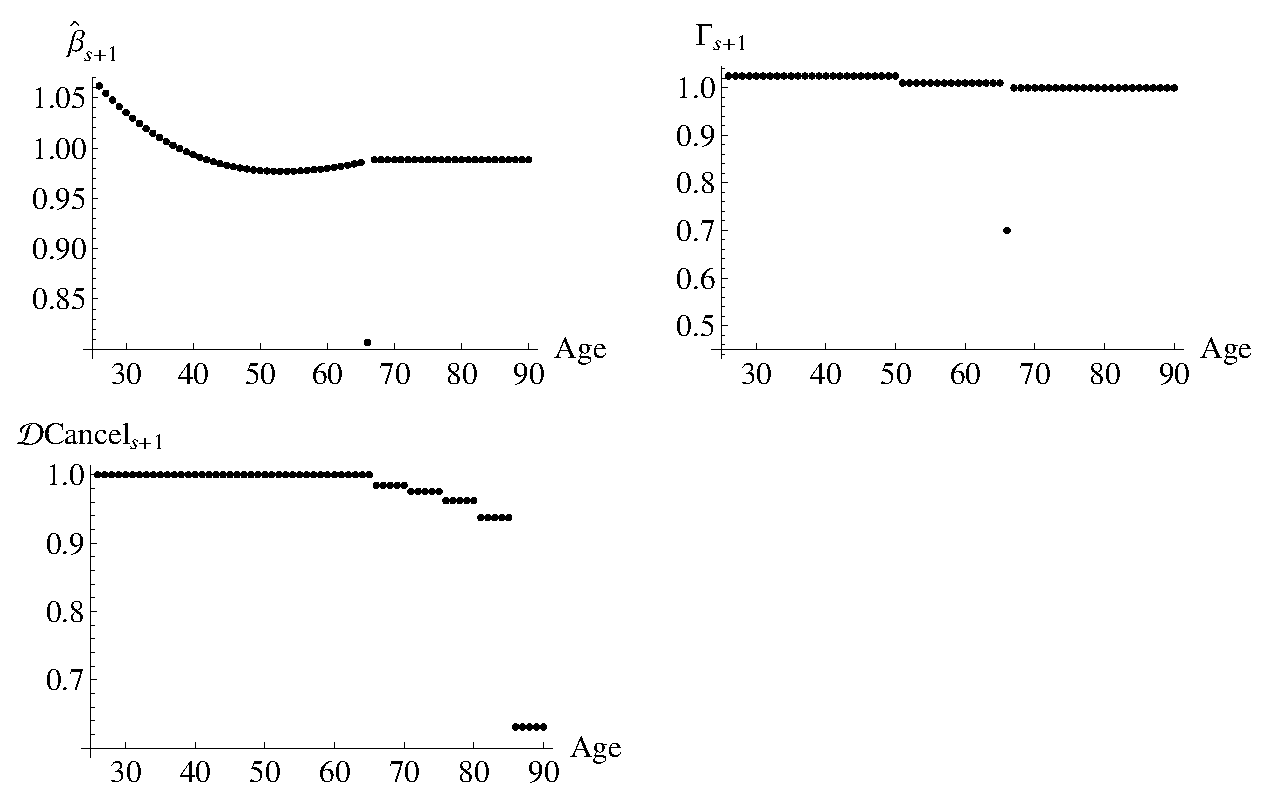
\includegraphics{./Figures/PlotTimeVaryingParam}
  \caption{Time Varying Parameters}
  \label{fig:TimeVaryingParam}
\end{figure}

\begin{table}[h]
  \caption{Parameter Values}\label{table:StrEstParams}
  \begin{center}
    \begin{tabular}{ccl}
      \hline\hline
      $\sigma _{\TranShkEmp}$    & $0.1$ & Carroll~\citeyearpar{carroll:brookings}
      \\ $\sigma _{\PermShk}$   & $0.1$ & Carroll~\citeyearpar{carroll:brookings}
      \\ $\pZero$           & $0.005$  & Carroll~\citeyearpar{carroll:brookings}
      \\ $\PermGroFac_{s}$        & figure \ref{fig:TimeVaryingParam} & Carroll~\citeyearpar{carrollBSLCPIH}
      \\ $\hat{\DiscFac}_{s},\Alive_{s}$ & figure \ref{fig:TimeVaryingParam} & Cagetti~\citeyearpar{cagettiWprofiles}
      \\$\Rfree$            & $1.03$  & Cagetti~\citeyearpar{cagettiWprofiles}\\
      \hline
    \end{tabular}
  \end{center}
\end{table}

The parameters ${\beth}$ and $\CRRA$ are structurally estimated following the procedure described below.

\subsection{Estimation}

When economists say that they are performing ``structural estimation''
of a model like this, they mean that they have devised a
formal procedure for searching for values for the parameters ${\beth}$
and $\CRRA$ at which some measure of the model's outcome (like
``median wealth by age'') is as close as possible to an empirical measure
of the same thing. Here, we choose to match the median of the
wealth to permanent income ratio across 7 age groups, from age $26-30$
up to $56-60$.\footnote{\cite{cagettiWprofiles}
  matches wealth levels rather than wealth to income ratios. We
  believe it is more appropriate to match ratios both because the
  ratios are the state variable in the theory and because empirical
  moments for ratios of wealth to income are not influenced by the
  method used to remove the effects of inflation and productivity
  growth.} The choice of matching the medians rather the means is
motivated by the fact that the wealth distribution is much more
concentrated at the top than the model is capable of explaining using a single
set of parameter values.  This means that in practice one must pick
some portion of the population who one wants to match well; since the
model has little hope of capturing the behavior of Bill Gates, but
might conceivably match the behavior of Homer Simpson, we choose to
match medians rather than means.

As explained in section \ref{sec:normalization}, it is convenient to work with the normalized version of the model which can be written in Bellman form as:
\begin{verbatimwrite}{./Equations/LifeCycleMaxNormed.tex}
  \begin{equation*}\begin{gathered}\begin{aligned}
        {\vFunc}_{t}({m}_{t})  & = \max_{{c}_{t}}~~~ \uFunc({c}_{t})+\beth\Alive_{t+1}\hat{\DiscFac}_{t+1}
          \Ex_{t}[(\PermShk_{t+1}\PermGroFac_{t+1})^{1-\CRRA}{\vFunc}_{t+1}({m}_{t+1})]   \\
        & \text{s.t.} &   \nonumber \\
        {a}_{t}    & = {m}_{t}-{c}_{t} \nonumber
        \\      {m}_{t+1}  & = {a}_{t}\underbrace{\left(\frac{\Rfree}{\PermShk_{t+1}\PermGroFac_{t+1}}\right)}_{\equiv \RNrm_{t+1}}+ ~\TranShkEmp_{t+1}
      \end{aligned}\end{gathered}\end{equation*}
\end{verbatimwrite}
\begin{eqnarray*}
    {\vFunc}_{t}({m}_{t}) & = & \max_{{c}_{t}} \left\{\util({c}_{t})+\beth\Alive_{t+1}\hat{\Discount}_{t+1}
    \Ex_{t}[(\pShk_{t+1}\PGro_{t+1})^{1-\CRRA}{\vFunc}_{t+1}({m}_{t+1})] \right\}   \\
         & \text{s.t.} &   \nonumber \\
    {a}_{t}   & = & {m}_{t}-{c}_{t} \nonumber
\\      {m}_{t+1} & = & {a}_{t}\underbrace{\left(\frac{\Rfree}{\pShk_{t+1}\PGro_{t+1}}\right)}_{\equiv \Rnorm_{t+1}}+\tShkEmp_{t+1}
\end{eqnarray*}
\unskip
with the first order condition:
\begin{verbatimwrite}{./Equations/FOCLifeCycle}
\begin{equation}\begin{gathered}\begin{aligned}
      \uFunc^{{c}}({c}_{t}) & = \beth\Alive_{t+1}\hat{\DiscFac}_{t+1}\Rfree \Ex_{t}\left[\uFunc^{{c}}\left(\PermShk_{t+1}\PermGroFac_{t+1}\cFunc_{t+1}\left({a}_{t}\RNrm_{t+1}+\TranShkEmp_{t+1}\right)\right)\right]\label{eq:FOCLifeCycle}
      .
    \end{aligned}\end{gathered}\end{equation}
\end{verbatimwrite}
\begin{equation}\begin{gathered}\begin{aligned}
      \uFunc^{{c}}({c}_{t}) & = \beth\Alive_{t+1}\hat{\DiscFac}_{t+1}\Rfree \Ex_{t}\left[\uFunc^{{c}}\left(\PermShk_{t+1}\PermGroFac_{t+1}\cFunc_{t+1}\left({a}_{t}\RNrm_{t+1}+\TranShkEmp_{t+1}\right)\right)\right]\label{eq:FOCLifeCycle}
      .
    \end{aligned}\end{gathered}\end{equation}


The first step is to solve for the consumption functions at each age
using the routines included in the \texttt{setup\_ConsFn.m} file. We
need to discretize the shock distribution and solve for the policy
functions by backward induction using equation (\ref{eq:FOCLifeCycle})
following the procedure in sections \ref{sec:NextToLast} and
\ref{sec:recursion} (\texttt{ConstructcFuncLife}). The latter routine
is slightly complicated by the fact that we are considering a
life-cycle model and therefore the growth rate of permanent income,
the probability of death, the time-varying discount factor and the
distribution of shocks will be different across the years. We thus
must ensure that at each backward iteration the right parameter
values are used.

Once we have the age varying consumption functions, we can proceed to
generate the simulated data and compute the simulated medians using
the routines defined in the \texttt{setup\_Sim.m} file. We first have
to draw the shocks for each agent and period. This involves
discretizing the shock distribution for as many points as the number
of agents we want to simulate
(\texttt{ConstructShockDistribution}). We then randomly permute this
shock vector as many times as we need to simulate the model for, thus
obtaining a time varying shock for each agent
(\texttt{ConstructSimShocks}). This is much more time efficient than
drawing at each time from the shock distribution a shock for each
agent, and also ensures a stable distribution of shocks across the
simulation periods even for a small number of agents. (Similarly, in
order to speed up the process, at each backward iteration we compute
the consumption function and other variables as a vector at once.)
Then, following Cagetti ~\citeyearpar{cagettiWprofiles}, we
initialize the wealth-to-income ratio of agents at age $25$ by
randomly assigning the equal probability values to $0.17$, $0.50$ and
$0.83$ and run the simulation (\texttt{Simulate}). In particular we
consider a population of agents at age 25 and follow their consumption
and wealth accumulation dynamics as they reach the age of $60$, using
the appropriate age-specific consumption functions and the age-varying
parameters. The simulated medians are obtained by taking the medians
of the wealth to income ratio of the $7$ age groups.

Given these simulated medians, we can estimate the model by
calculating empirical medians and measure the model's success
by calculating the difference between the empirical median and the
actual median.  Specifically, defining $\xi$ as the set of parameters
to be estimated (in the current case $\xi =\{\CRRA ,{\beth}\}$), we could search for
the parameter values which solve
\begin{verbatimwrite}{./Equations/naivePowell.tex}
  \begin{equation}
    \begin{gathered}
      \begin{aligned}
        \min_{\xi} \sum_{\tau=1}^{7} |\varsigma^{\tau} -\mathbf{s}^{\tau}(\xi)|  \label{eq:naivePowell}
      \end{aligned}
    \end{gathered}
  \end{equation}
\end{verbatimwrite}
  \begin{equation}\begin{gathered}\begin{aligned}
        \min_{\xi} \sum_{\tau=1}^{7} |\varsigma^{\tau} -\mathbf{s}^{\tau}(\xi)|  \label{eq:naivePowell}
      \end{aligned}\end{gathered}\end{equation}
\unskip
where $\varsigma^{\tau }$ and $\mathbf{s}^{\tau}$ are respectively the empirical and simulated medians of the wealth to permanent income ratio for age group $\tau $.

A drawback of proceeding in this way is that it treats the empirically
estimated medians as though they reflected perfect measurements of the
truth. Imagine, however, that one of the age groups happened to have
(in the consumer survey) four times as many data observations as
another age group; then we would expect the median to be more
precisely estimated for the age group with more observations; yet
\eqref{eq:naivePowell} assigns equal importance to a deviation between
the model and the data for all age groups.

We can get around this problem (and a variety of others) by instead minimizing a slightly more complex object:
\begin{verbatimwrite}{./Equations/StructEstim.tex}
  \begin{equation}
    \min_{\xi}\sum\limits_{i}^{N}\weight _{i}\left|\varsigma_{i}^{\tau }-\mathbf{s}^{\tau}(\xi )\right|\label{eq:StructEstim}
  \end{equation}
\end{verbatimwrite}
\begin{equation}
    \min_{\xi}\sum\limits_{i}^{N}\weight _{i}\left|\varsigma_{i}^{\tau }-\mathbf{s}^{\tau}(\xi )\right|\label{eq:StructEstim}
\end{equation}
\unskip
where $\weight_{i}$ is the weight of household $i$ in the entire
population,\footnote{The Survey of Consumer Finances includes many
  more high-wealth households than exist in the population as a whole;
  therefore if one wants to produce population-representative
  statistics, one must be careful to weight each observation by the
  factor that reflects its ``true'' weight in the population.} and
$\varsigma_{i}^{\tau }$ is the empirical wealth-to-permanent-income
ratio of household $i$ whose head belongs to age group
$\tau$. $\weight _{i}$ is needed because unequal weight is assigned to
each observation in the Survey of Consumer Finances (SCF). The
absolute value is used since the formula is based on the fact that the
median is the value that minimizes the sum of the absolute deviations
from itself.

% In the absence of observation specific weights, equation (\ref{eq:MinStructEstim}) can be simplified to require the minimization of the distance between the empirical and simulated medians.

The actual data are taken from several waves of the SCF and the medians and means for each age category are plotted in figure \ref{fig:MeanMedianSCF}. More details on the SCF data are included in appendix \ref{app:SCFdata}.
\hypertarget{PlotMeanMedianSCFcollegeGrads}{}
\begin{figure}
  % 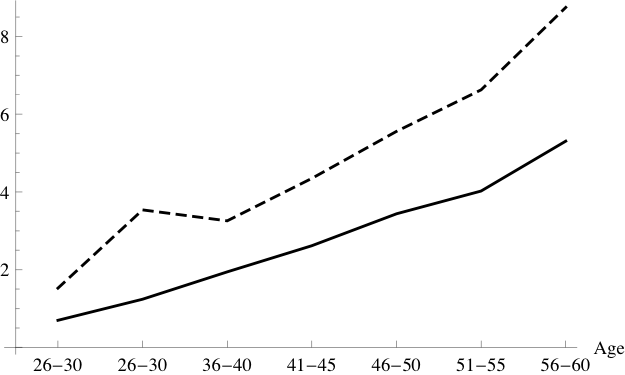
\includegraphics{./Figures/PlotMeanMedianSCF}} % weird mean value
  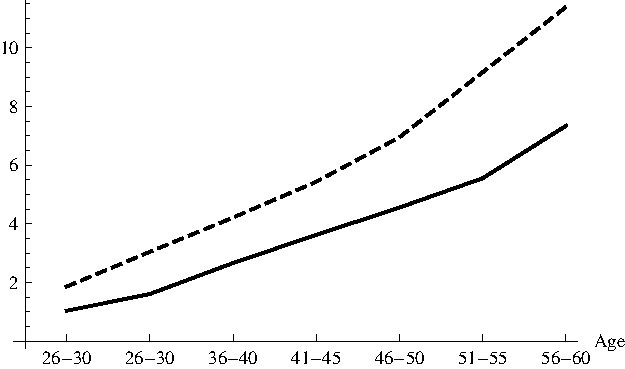
\includegraphics{./Figures/PlotMeanMedianSCFcollegeGrads}
  \caption{Wealth to Permanent Income Ratios from SCF (means (dashed) and medians (solid))}
  \label{fig:MeanMedianSCF}
\end{figure}

The key function to perform structural estimation is defined in the \texttt{setup\_Estimation.m} file as follows:
\begin{verbatimwrite}{./Equations/GapEmpiricalSimulatedMedians.tex}
  \begin{equation}\begin{gathered}\begin{aligned}
        \lefteqn{    \texttt{GapEmpiricalSimulatedMedians$[\CRRA,\beth]$:=}}    \nonumber \\
        &[&\texttt{ConstructcFuncLife$[\CRRA,\beth]$;}\nonumber\\
        &\texttt{Simulate;}\nonumber\\
        &\sum\limits_{i}^{N}\weight _{i}\left|\varsigma_{i}^{\tau }-\mathbf{s}^{\tau}(\xi )\right| \nonumber\\
        &];&\nonumber
      \end{aligned}\end{gathered}\end{equation}
\end{verbatimwrite}
  \begin{equation}\begin{gathered}\begin{aligned}
        \lefteqn{    \texttt{GapEmpiricalSimulatedMedians$[\CRRA,\beth]$:=}}    \nonumber \\
        &[&\texttt{ConstructcFuncLife$[\CRRA,\beth]$;}\nonumber\\
        &\texttt{Simulate;}\nonumber\\
        &\sum\limits_{i}^{N}\weight _{i}\left|\varsigma_{i}^{\tau }-\mathbf{s}^{\tau}(\xi )\right| \nonumber\\
        &];&\nonumber
      \end{aligned}\end{gathered}\end{equation}
\unskip
For a given pair of the parameters to be estimated, the \texttt{GapEmpiricalSimulatedMedians} routine therefore:
\begin{enumerate}
\item solves for the consumption functions by calling \texttt{ConstructcFuncLife}
\item simulates the data and computes the simulated medians by calling \texttt{Simulate}
\item returns the value of equation (\ref{eq:StructEstim})
\end{enumerate}

We delegate the task of finding the coefficients that minimize the
\texttt{GapEmpiricalSimulatedMedians} function to the \Mma~
built-in numerical minimizer \texttt{FindMinimum}.  This task can be
quite time demanding and rather problematic if the
\texttt{GapEmpiricalSimulatedMedians} function has very flat regions
or sharp features. It is thus wise to verify the accuracy of the
solution, for example by experimenting with a variety of alternative starting values for the
parameter search.

Finally the standard errors are computed by bootstrap using the
routines in the \texttt{setup\_Bootstrap.m} file.\footnote{For a
  treatment of the advantages of the bootstrap see
  Horowitz~\citeyearpar{horowitzBootstrap}} This involves:
\begin{enumerate}
\item drawing new shocks for the simulation
\item drawing a random sample (with replacement) of actual data from the SCF
\item obtaining new estimates for $\CRRA$ and ${\beth}$
\end{enumerate}
We repeat the above procedure several times (\texttt{Bootstrap}) and take the standard deviation for each of the estimated parameters across the various bootstrap iterations.

The file \texttt{StructEstimation.m} produces our $\CRRA$ and
${\beth}$ estimates with standard errors using 10,000 simulated
agents.\footnote{The procedure is: First we calculate the $\CRRA$ and
  ${\beth}$ estimates as the minimizer of equation
  (\ref{eq:StructEstim}) using the actual SCF data. Then, we apply the
  \texttt{Bootstrap} function several times to obtain the standard
  error of our estimates.} Results are reported in Table
\ref{tab:EstResults}.\footnote{Differently from Cagetti
  ~\citeyearpar{cagettiWprofiles} who estimates a different set of
  parameters for college graduates, high school graduates and high
  school dropouts graduates, we perform the structural estimation on
  the full population.} Figure \ref{fig:PlotContourMedianStrEst} shows
the contour plot of the \texttt{GapEmpiricalSimulatedMedians} function
and the parameter estimates. The contour plot shows equally spaced
isoquants of the \texttt{GapEmpiricalSimulatedMedians} function,
i.e.\ the pairs of $\CRRA$ and ${\beth}$ which lead to the same
deviations between simulated and empirical medians (equivalent values
of equation (\ref{eq:StructEstim})). We can thus interestingly see
that there is a large rather flat region, or more formally speaking
there exists a broad set of parameter pairs which leads to similar
simulated wealth to income ratios. Intuitively, the flatter and larger
is this region, the harder it is for the structural estimation
procedure to precisely identify the parameters.
\begin{verbatimwrite}{./Tables/EstResults.tex}
  \begin{table}[h]
    \caption{Estimation Results}\label{tab:EstResults}
    \center
    \begin{tabular}{cc}
      \hline
      $\CRRA $ & ${\beth}$\\
      \hline
      $4.68$ & $1.00$\\
      $(0.13)$ & $(0.00)$\\
      \hline
    \end{tabular}
  \end{table}
\end{verbatimwrite}
    \begin{table}[h]
      \caption{Estimation Results}\label{tab:EstResults}
      \center
      \begin{tabular}{cc}
        \hline
        $\CRRA $ & ${\beth}$\\
        \hline
        $4.68$ & $1.00$\\
        $(0.13)$ & $(0.00)$\\
        \hline
      \end{tabular}
    \end{table}
  
\unskip

\hypertarget{PlotContourMedianStrEst}{}
\begin{figure}
  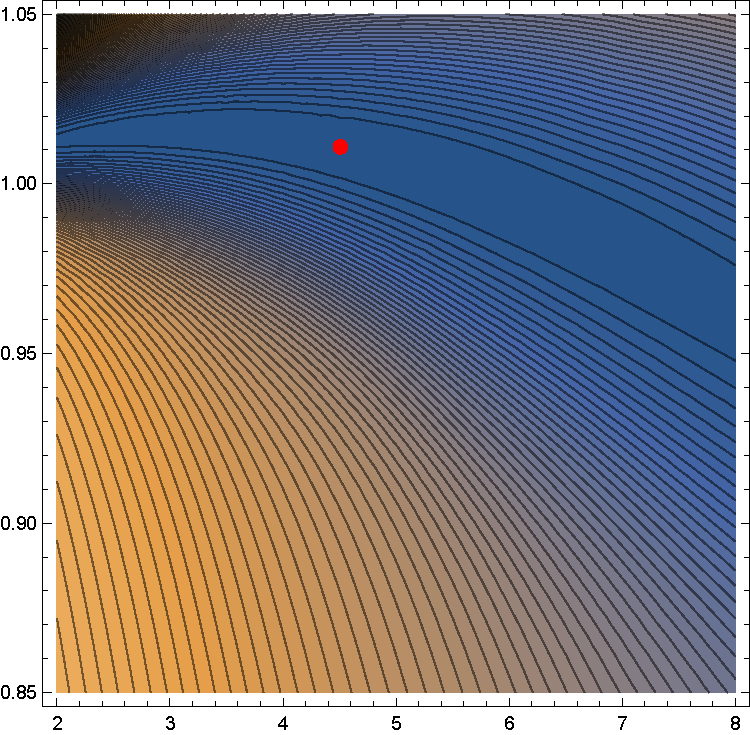
\includegraphics{./Figures/PlotContourMedianStrEst}
  \caption{Contour Plot (larger values are shown lighter) with $\{\CRRA,{\beth}\}$ Estimates (red dot).}
  \label{fig:PlotContourMedianStrEst}
\end{figure}

\section{Conclusion}

There are many choices that can be made for solving microeconomic dynamic stochastic optimization problems.  The set of techniques, and associated programs, described in these notes represents an approach that I have found to be powerful, flexible, and efficient, but other problems may require other techniques.  For a much broader treatment of many of the issues considered here, see Judd~\citeyearpar{judd:book}.

\clearpage\vfill\eject

\appendix

\centerline{\LARGE Appendices}\vspace{0.2in}

\section{Further Details on SCF Data}\label{app:SCFdata}

Data used in the estimation is constructed using the SCF 1992, 1995, 1998, 2001 and 2004 waves. The definition of wealth is net worth including housing wealth, but excluding pensions and social securities. The data set contains only households whose heads are aged 26-60 and excludes singles, following Cagetti~\citeyearpar{cagettiWprofiles}.\footnote{Cagetti~\citeyearpar{cagettiWprofiles}\ argues that younger households should be dropped since educational choice is not modeled. Also, he drops singles, since they include a large number of single mothers whose saving behavior is influenced by welfare.} Furthermore, the data set contains only households whose heads are college graduates. The total sample size is 4,774.

In the waves between 1995 and 2004 of the SCF, levels of
\textit{normal} income are reported. The question in the questionnaire
is "About what would your income have been if it had been a normal
year?" We consider the level of normal income as corresponding to the
model's theoretical object $P$, permanent noncapital income. Levels of
normal income are not reported in the 1992 wave. Instead, in this wave
there is a variable which reports whether the level of income is
normal or not. Regarding the 1992 wave, only observations which report
that the level of income is normal are used, and the levels of income
of remaining observations in the 1992 wave are interpreted as the
levels of permanent income.

Normal income levels in the SCF are before-tax figures. These
before-tax permanent income figures must be rescaled so that the median of
the rescaled permanent income of each age group matches the median of
each age group's income which is assumed in the simulation. This
rescaled permanent income is interpreted as after-tax permanent
income. This rescaling is crucial since in the estimation empirical
profiles are matched with simulated ones which are generated using
after-tax permanent income (remember the income process assumed in the
main text). Wealth / permanent income ratio is computed by dividing
the level of wealth by the level of (after-tax) permanent income, and
this ratio is used for the estimation.\footnote{Please refer to the archive code for details of
  how these after-tax measures of $P$ are constructed.}

\vfill\clearpage

\write18{if [ ! -f \texname.bib ]; then touch \texname.bib  ; fi}\write18{if [ ! -f \texname-Add.bib ]; then touch \texname-Add.bib  ; fi}\bibliography{economics,\texname,\texname-Add}

\trp{
\pagebreak
\hypertarget{Appendices}{} % Allows link to [url-of-paper]#Appendices
\ifthenelse{\boolean{Web}}{}{% Web version has no page headers
  \chead[Appendices]{Appendices}      % but PDF version does
  \appendixpage % Reset formatting for appendices
} 
\appendix
\addcontentsline{toc}{section}{Appendices} % Say "Appendices"

\subfile{TRP_aInU}
}{}


\end{document}

% Local Variables:
% TeX-master-file: t
% eval: (setq TeX-command-list  (assq-delete-all (car (assoc "BibTeX" TeX-command-list)) TeX-command-list))
% eval: (setq TeX-command-list  (assq-delete-all (car (assoc "Biber"  TeX-command-list)) TeX-command-list))
% eval: (setq TeX-command-list  (remove '("BibTeX" "%(bibtex) %s"    TeX-run-BibTeX nil t :help "Run BibTeX") TeX-command-list))
% eval: (setq TeX-command-list  (remove '("BibTeX"    "bibtex %s"    TeX-run-BibTeX nil (plain-tex-mode latex-mode doctex-mode ams-tex-mode texinfo-mode context-mode)  :help "Run BibTeX") TeX-command-list))
% eval: (setq TeX-command-list  (remove '("BibTeX" "bibtex %s"    TeX-run-BibTeX nil t :help "Run BibTeX") TeX-command-list))
% eval: (add-to-list 'TeX-command-list '("BibTeX" "bibtex %s" TeX-run-BibTeX nil t                                                                              :help "Run BibTeX") t)
% eval: (add-to-list 'TeX-command-list '("BibTeX" "bibtex %s" TeX-run-BibTeX nil (plain-tex-mode latex-mode doctex-mode ams-tex-mode texinfo-mode context-mode) :help "Run BibTeX") t)
% TeX-PDF-mode: t
% TeX-file-line-error: t
% TeX-debug-warnings: t
% LaTeX-command-style: (("" "%(PDF)%(latex) %(file-line-error) %(extraopts) -output-directory=. %S%(PDFout)"))
% TeX-source-correlate-mode: t
% TeX-parse-self: t
% TeX-parse-all-errors: t
% eval: (cond ((string-equal system-type "darwin") (progn (setq TeX-view-program-list '(("Skim" "/Applications/Skim.app/Contents/SharedSupport/displayline -b %n %o %b"))))))
% eval: (cond ((string-equal system-type "gnu/linux") (progn (setq TeX-view-program-list '(("Evince" "evince --page-index=%(outpage) %o"))))))
% eval: (cond ((string-equal system-type "gnu/linux") (progn (setq TeX-view-program-selection '((output-pdf "Evince"))))))
% End:
